\documentclass[11pt]{article}

% -------------------- PACKAGES --------------------
\usepackage[a4paper, margin=1in]{geometry}
\usepackage{setspace}
\usepackage{amsmath, amssymb, amsthm}
\usepackage{graphicx}
\usepackage{booktabs}
\usepackage[authoryear,round]{natbib}
\usepackage{hyperref}
\hypersetup{pdftitle={Algorithmic Collusion in Financial Markets}, pdfauthor={Clemente Esquinas Coves}}
\usepackage{float}
\usepackage{caption}
\usepackage{parskip}
\usepackage{subcaption}
\usepackage{listings}
\usepackage{xcolor}
\usepackage[T1]{fontenc}

\definecolor{codebg}{rgb}{0.97,0.97,0.97}
\definecolor{codekw}{rgb}{0.0,0.0,0.6}
\definecolor{codestr}{rgb}{0.6,0.0,0.0}
\definecolor{codecmt}{rgb}{0.25,0.5,0.35}

\lstdefinestyle{pythonstyle}{
    language=Python,
    basicstyle=\ttfamily\footnotesize,
    keywordstyle=\color{codekw}\bfseries,
    stringstyle=\color{codestr},
    commentstyle=\color{codecmt}\itshape,
    backgroundcolor=\color{codebg},
    numbers=left,
    numberstyle=\tiny\color{gray},
    numbersep=6pt,
    frame=single,
    framesep=4pt,
    rulecolor=\color{gray!30},
    breaklines=true,
    breakatwhitespace=false,
    postbreak=\mbox{\textcolor{red}{$\hookrightarrow$}\space},
    showstringspaces=false,
    tabsize=4,
    captionpos=b,
    upquote=true,
    literate={—}{{--}}1 {–}{{-}}1 {≈}{{$\approx$}}1 {≥}{{$\geq$}}1
             {≤}{{$\leq$}}1 {α}{{$\alpha$}}1 {β}{{$\beta$}}1
             {γ}{{$\gamma$}}1 {θ}{{$\theta$}}1 {λ}{{$\lambda$}}1
             {ξ}{{$\xi$}}1 {ρ}{{$\rho$}}1 {σ}{{$\sigma$}}1
             {χ}{{$\chi$}}1 {ε}{{$\epsilon$}}1 {Δ}{{$\Delta$}}1
             {π}{{$\pi$}}1 {²}{{\textsuperscript{2}}}1
}

\lstdefinestyle{outputstyle}{
    basicstyle=\ttfamily\footnotesize,
    backgroundcolor=\color{codebg!50},
    frame=single,
    framesep=4pt,
    rulecolor=\color{gray!20},
    breaklines=true,
    breakatwhitespace=false,
    postbreak=\mbox{\textcolor{red}{$\hookrightarrow$}\space},
    showstringspaces=false,
    tabsize=4,
    upquote=true,
    literate={—}{{--}}1 {–}{{-}}1 {≈}{{$\approx$}}1 {≥}{{$\geq$}}1
             {≤}{{$\leq$}}1 {α}{{$\alpha$}}1 {β}{{$\beta$}}1
             {γ}{{$\gamma$}}1 {θ}{{$\theta$}}1 {λ}{{$\lambda$}}1
             {ξ}{{$\xi$}}1 {ρ}{{$\rho$}}1 {σ}{{$\sigma$}}1
             {χ}{{$\chi$}}1 {ε}{{$\epsilon$}}1 {Δ}{{$\Delta$}}1
             {π}{{$\pi$}}1 {²}{{\textsuperscript{2}}}1
}

\onehalfspacing

\begin{document}

\begin{titlepage}
    \centering
    \vspace*{6cm}
    
    {\Huge\bfseries Algorithmic Collusion in\\Financial Markets\par}
    \vspace{1cm}
    
    {\Large Q-Learning Speculators in a Kyle Model with\\Information-Insensitive Investors\par}
    \vspace{5cm}
    
    {\Large\bfseries Clemente Esquinas Coves\par}
    \vspace{0.5cm}
    
    {\large May 2026\par}
    
    \vfill
    
\end{titlepage}

% -------------------- SECTIONS --------------------

\section{Introduction}

The rapid adoption of autonomous, model-free algorithms in financial
markets has raised a concern: can self-interested algorithms
learn to collude without explicit communication or pre-programmed
intent? Recent work by \citet{Dou2025} suggests that the answer is yes, at
least in controlled settings that preserve the essential
informational structure of securities trading. This project revisits
their framework, first characterizing the theoretical benchmarks
analytically and then assessing whether Q-learning speculators trading
against one another converge to collusive outcomes. The model extends
the canonical \citet{Kyle1985} setup with multiple symmetric informed
speculators trading in parallel and a continuum of
information-insensitive investors who trade mechanically against the
price; the friction introduced by the latter is what opens the door to
sustainable collusion when present.

The report proceeds in three parts. Section~3 derives the linear Nash
and cartel equilibria, yielding closed-form expressions for trading
intensity $\chi$, price impact $\lambda$, and per-speculator profit at
$\xi = 0$, and shows that the cartel earns higher per-speculator profit
than Nash for $I \geq 2$. Section~4 develops the market-quality
analysis: liquidity $\mathcal{L} = 1/\lambda$, price informativeness
$\mathcal{I}$, and noise-trader losses $W_N$, with comparative statics
in $I$ at $\xi = 0$ and $\xi = 500$, and a discussion of the effective
number of insiders $I^*$. Section~5 implements the Q-learning protocol
of \citet{Dou2025}, measures the collusion index $\Delta_\chi$ in both
regimes, and uses a noise-shock impulse response analysis to
distinguish collusion sustained by price-trigger strategies from
collusion sustained by over-pruning bias.

\section{Model}

Consider a repeated market for a risky asset with fundamental value 
$v_t \sim \mathcal{N}(\bar{v}, \sigma_v^2)$, drawn independently each period. 
There are four types of participants:

\begin{enumerate}
    \item \textbf{Informed speculators.} There are $I \geq 1$ symmetric informed speculators. 
    Each speculator $i$ observes $v_t$ at the beginning of period $t$ and submits a market order $x_{i,t}$. 
    Speculator $i$'s profit in period $t$ is
    \[
    \boxed{\pi_{i,t} = (v_t - p_t)x_{i,t}}.
    \]

    \item \textbf{Noise trader.} A noise trader submits orders 
    $u_t \sim \mathcal{N}(0, \sigma_u^2)$, independent of $v_t$ and across periods.

    \item \textbf{Information-insensitive investors.} Information-insensitive investors have aggregate demand
    \begin{equation}
        \boxed{z_t = -\xi (p_t - \bar{v}), \quad \xi \geq 0}.
    \end{equation}
    
    When $\xi = 0$ the model reduces to the standard Kyle framework. 
    When $\xi > 0$, these investors buy when the price is below $\bar{v}$ 
    and sell when it is above, without inferring information from prices.

    \item \textbf{Market maker.} The market maker observes the total order flow 
    \[
    \boxed{y_t = \sum_{i=1}^I x_{i,t} + u_t}
    \]
    and the information-insensitive investor demand $z_t$. 
    The market maker sets the price to minimize 
    a weighted combination of pricing errors and inventory costs:
    \begin{equation}
        \boxed{p_t = \arg\min_p \ \theta \big(p - \mathbb{E}[v_t \mid y_t]\big)^2 + (y_t + z_t)^2},
        \label{mm_opt}
    \end{equation}
    where $\theta > 0$ governs the relative weight on price discovery.
    
    The resulting linear pricing rule takes the form
    \begin{equation}
        \boxed{p_t = \bar{v} + \lambda y_t}.
        \label{pricingrule}
    \end{equation}
\end{enumerate}

\section{Equilibrium Analysis}
\subsection{Pricing Rule}
To derive the pricing rule, we solve the market maker's optimization problem (\ref{mm_opt}) by minimizing the following expression with respect to $p$:
\[
X(p)=\theta(p-\mathbb{E}[v_t\mid y_t])^2+(y_t-\xi(p-\bar{v}))^2.
\]
To find the optimal price, we differentiate $X$ with respect to $p$ and set it to zero:
\[
\frac{dX}{dp}=2\theta(p^*-\mathbb{E}[v_t\mid y_t])-2\xi(y_t-\xi(p^*-\bar{v}))=0\iff
\]
\[
\iff \theta p^*-\theta\mathbb{E}[v_t\mid y_t]-\xi y_t+\xi^2p^*-\xi^2\bar{v}=0\iff p^*=\frac{\xi^2 \bar{v}}{\theta + \xi^2}+\frac{\xi y_t}{\theta + \xi^2}+\frac{\theta \mathbb{E}[v_t\mid y_t]}{\theta + \xi^2}.
\]
Now, by assumption, $v_t=\bar{v}+\gamma y_t+\varepsilon_t$, where $\gamma=\mathbb{E}[v_t-\bar{v}\mid y_t]$ is the regression coefficient of $v_t$ on $y_t$, and $\varepsilon_t$ is uncorrelated with $y_t$. Therefore:
\[
\mathbb{E}[v_t\mid y_t]=\mathbb{E}[\bar{v}\mid y_t]+\gamma \mathbb{E}[y_t\mid y_t]+\mathbb{E}[\varepsilon_t\mid y_t]=\bar{v}+\gamma y_t,
\]
since $\bar{v}$ is a constant, $y_t$ is $y_t-$known and $\varepsilon_t$ is the residual of the regression which must have expectation zero. Also, $\mathbb{E}[\varepsilon_t\mid y_t]=\mathbb{E}[\varepsilon_t]$ because normality makes uncorrelatedness equivalent to independence: $y_t$ is a linear combination of $v_t$ and $u_t$ (both Gaussian and independent), and $\varepsilon_t$ is also a linear combination of $v_t$ and $u_t$, so $(\varepsilon_t,y_t)$ is jointly normal.

Hence, we get:
\[
p^*=\frac{\xi^2 \bar{v}}{\theta + \xi^2}+\frac{\xi y_t}{\theta + \xi^2}+\frac{\theta (\bar{v}+\gamma y_t)}{\theta + \xi^2}=\bar{v}+\frac{\gamma \theta+\xi}{\theta+\xi^2}y_t=\bar{v}+\lambda y_t.
\]
Additionally:
\[
\frac{d^2X}{dp^2}=2\theta+2\xi^2>0,
\]
which confirms $p^*$ achieves a minimum. This yields the pricing rule (\ref{pricingrule}).


\subsection{Nash Equilibrium}
In the context of this model, a Nash equilibrium is a symmetric strategy such that no 
speculator can increase their expected profit by unilaterally deviating, taking the 
strategies of all other speculators as given. Here we derive speculator 
$i$'s best response and impose symmetry to characterize the Nash equilibrium.

Suppose each speculator $i$ uses a linear strategy $x_{i,t}=\chi_i(v_t-\bar{v})$. 
Speculator $i$'s profit in period $t$ is therefore $\pi_{i,t}=(v_t-p_t)\chi_i(v_t-\bar{v})$. Substituting the pricing rule (\ref{pricingrule}):
\[
\pi_{i,t}=(v_t-\bar{v}-\lambda y_t)\chi_i(v_t-\bar{v}).
\]
Now, fixing the strategies of all speculators $j\neq i$ at intensity $\chi$, we obtain $y_t=(I-1)\chi(v_t-\bar{v})+\chi_i(v_t-\bar{v})+u_t.$ Substituting into the expression for $\pi_{i,t}$:
\[
\pi_{i,t}=\chi_i(v_t-\bar{v})\left(v_t-\bar{v}-\lambda(\chi(I-1)(v_t-\bar{v})+\chi_i(v_t-\bar{v})+u_t)\right).
\]
Expanding the expression for $\pi_{i,t}$:
\[
\pi_{i,t}=\chi_i(v_t-\bar{v})^2-\lambda \chi_i(v_t-\bar{v})\left[\chi(I-1)(v_t-\bar{v})+u_t\right]-\lambda \chi_i^2(v_t-\bar{v})^2=
\]
\[
=(v_t-\bar{v})^2\left[\chi_i-\lambda\chi_i\chi(I-1)-\lambda \chi_i^2\right]-\lambda \chi_i(v_t-\bar{v})u_t.
\]
The best response is given by the expected profit $P(\lambda,\chi,\chi_i)$ conditioned 
on the fundamental value of the risky asset at time $t$, so:
\[
P(\lambda,\chi,\chi_i)=\mathbb{E}[\pi_{i,t}(\lambda, \chi,\chi_i)\mid v_t]=(v_t-\bar{v})^2\left[\chi_i-\lambda \chi_i\chi (I-1)-\lambda \chi_i^2\right].
\]
This last equality is due to $(v_t-\bar{v})$ being $v_t-$known and 
$\mathbb{E}[(v_t-\bar{v})u_t\mid v_t]=(v_t-\bar{v})\mathbb{E}[u_t]=0$ 
($u_t$ is independent of $v_t$). Taking the first order condition of $P(\lambda,\chi,\chi_i)$ with respect to $\chi_i$ 
(where we assume $\lambda>0$, as will be verified below):
\[
\frac{\partial P}{\partial \chi_i}=(v_t-\bar{v})^2\left[1-\lambda \chi(I-1)-2\lambda\chi_i\right]=0\iff 1-\lambda \chi(I-1)-2\lambda\chi_i^*=0
\]
\[
\iff 2\lambda \chi_i^*=1-\lambda \chi(I-1)\iff \chi_i^*=\frac{1}{2\lambda}-\frac{\chi(I-1)}{2}.
\]

Lastly, imposing the symmetry of the Nash equilibrium condition $\chi_i=\chi$:
\[
\chi^N=\frac{1}{2\lambda^N}-\frac{\chi^N(I-1)}{2}\iff \chi^N\left(1+\frac{I-1}{2}\right)=\frac{1}{2\lambda^N}\iff
\]
\begin{equation}
    \chi^N=\frac{1}{(I+1)\lambda^N},
\end{equation}
which is the first condition of the Nash equilibrium.

From the definition of $\lambda$:
\begin{equation}
    \lambda^N=\frac{\theta \gamma^N+\xi}{\theta+\xi^2}.
\end{equation}

Since $\gamma$ is the regression coefficient of $v_t$ on $y_t$:
\begin{equation}
    \gamma=\frac{\text{Cov}(v_t,y_t)}{\text{Var}(y_t)}.
\end{equation}
In this equilibrium, $y_t=I\chi^N(v_t-\bar{v})+u_t$, hence:
\[
\text{Cov}(v_t,y_t)=\text{Cov}(v_t,I\chi^N(v_t-\bar{v})+u_t)=\text{Cov}(v_t,I\chi^N v_t-I\chi^N \bar{v})=I\chi^N\text{Var}(v_t)=I\chi^N \sigma_v^2,
\]
since $u_t$ is independent of $v_t$ and $\bar{v}$ is a constant. Note that $\chi^N>0$ 
(speculators buy when $v_t>\bar{v}$ and sell when $v_t<\bar{v}$), therefore $\gamma>0$, 
which in turn implies $\lambda>0$, confirming our earlier assumption. Furthermore:
\[
\frac{\partial^2 P}{\partial \chi_i^2}=(v_t-\bar{v})^2(-2\lambda)<0,
\]
so the value we obtained for $\chi^N$ was indeed a maximum.

We now compute $\text{Var}(y_t)$:
\[
\text{Var}(y_t)=\text{Var}(I\chi^N(v_t-\bar{v})+u_t)=\text{Var}(I\chi^N v_t-I\chi^N \bar{v}+u_t)=\text{Var}(I\chi^N v_t+u_t)=I^2(\chi^N)^2\sigma_v^2+\sigma_u^2.
\]
Consequently:
\begin{equation}
    \gamma^N=\frac{I\chi^N \sigma_v^2}{I^2(\chi^N)^2\sigma_v^2+\sigma_u^2}=\frac{I\chi^N}{(I\chi^N)^2+(\sigma_u/\sigma_v)^2}.
\end{equation}
Finally, we derive the expected per-speculator profit. Substituting $p_t=\bar{v}+\lambda^N y_t$ 
and $x_{i,t}=\chi^N(v_t-\bar{v})$ into $\pi_{i,t}=(v_t-p_t)x_{i,t}$:
\[
\pi_{i,t}=\chi^N(v_t-\bar{v})(v_t-\bar{v}-\lambda^N y_t).
\]
Taking unconditional expectation and substituting $y_t = I\chi^N(v_t-\bar{v})+u_t$:
\[
\pi^N=\mathbb{E}\left[\chi^N(v_t-\bar{v})(v_t-\bar{v}-\lambda^N(I\chi^N(v_t-\bar{v})+u_t))\right]=\chi^N(1-\lambda^NI\chi^N)\mathbb{E}[(v_t-\bar{v})^2],
\]
since $(v_t-\bar{v})$ is independent of $u_t$ and $\mathbb{E}[u_t]=0$. This gives:
\begin{equation}
    \pi^N=(1-\lambda^NI\chi^N)\chi^N\sigma_v^2.
\end{equation}



\subsection{Cartel Equilibrium}
Now suppose all $I$ speculators form a cartel that maximizes the total profit of the group, namely, they all coordinate on the same intensity $\chi^M$ that maximizes:
\[
\sum_{i=1}^I\pi_{i,t}=(v_t-p_t)I\chi^M(v_t-\bar{v})
\]
Substituting $p_t=\bar{v}+\lambda^M y_t$ and $y_t=I\chi^M(v_t-\bar{v})+u_t$:
\[
\sum_{i=1}^I\pi_{i,t}=I\chi^M(v_t-\bar{v})^2-I\lambda^M\chi^M(v_t-\bar{v})(I\chi^M(v_t-\bar{v})+u_t)
\]
Taking the conditional expectation on $v_t$:
\[
Q:=\mathbb{E}\left[\sum_{i=1}^I\pi_{i,t}\mid v_t\right]=I\chi^M(v_t-\bar{v})^2-I^2\lambda^M(\chi^M)^2(v_t-\bar{v})^2-I\lambda^M\chi^M(v_t-\bar{v})\mathbb{E}[u_t\mid v_t]=
\]
\[
=I\chi^M(v_t-\bar{v})^2-I^2\lambda^M(\chi^M)^2(v_t-\bar{v})^2
\]
since $u_t$ is independent of $v_t$ and $\mathbb{E}[u_t]=0$.

Taking the first order condition with respect to $\chi^M$:
\[
\frac{\partial Q}{\partial \chi^M}=(v_t-\bar{v})^2\left[I-2I^2\lambda^M\chi^M\right]=0\iff
\]
\begin{equation}
    \chi^M=\frac{1}{2I\lambda^M}.
\end{equation}
Moreover (where $\lambda^M>0$ is verified below):
\[
\frac{\partial^2 Q}{\partial (\chi^M)^2}=(v_t-\bar{v})^2(-2I^2\lambda^M)<0,
\]
so it is indeed a maximum.

From the definition of $\lambda$:
\begin{equation}
    \lambda^M=\frac{\theta \gamma^M+\xi}{\theta+\xi^2}.
\end{equation}
The derivations of $\gamma^M$ and $\pi^M$ follow analogously to the Nash case, replacing $\chi^N$ and $\lambda^N$ with $\chi^M$ and $\lambda^M$. Note that $\lambda^M>0$ for the same reason as $\lambda^N$. Consequently:
\begin{equation}
    \gamma^M=\frac{I\chi^M}{(I\chi^M)^2+(\sigma_u/\sigma_v)^2},
\end{equation}
and
\begin{equation}
    \pi^M=(1-\lambda^MI\chi^M)\chi^M\sigma_v^2.
\end{equation}

\subsection{Closed Forms and Numerical Results}
When $\xi=0$, the expression for $\lambda^N$ simplifies to $\lambda^N = \gamma^N$. 
Substituting into the expression for $\chi^N$ and rearranging:
\[
\chi^N = \frac{1}{(I+1)\gamma^N} = \frac{1}{I+1}\cdot\frac{(I\chi^N)^2+(\sigma_u/\sigma_v)^2}{I\chi^N}.
\]
Multiplying both sides by $(I+1)\chi^N$:
\[
(I+1)I(\chi^N)^2 = I^2(\chi^N)^2 + \frac{\sigma_u^2}{\sigma_v^2} \implies (\chi^N)^2 = \frac{\sigma_u^2}{I\sigma_v^2},
\]
and therefore:
\begin{equation}
    \chi^N = \frac{\sigma_u}{\sqrt{I}\sigma_v}.
    \label{nash_chi}
\end{equation}
Substituting into $\lambda^N = \gamma^N = \frac{I\chi^N}{(I\chi^N)^2+(\sigma_u/\sigma_v)^2}$:
\[
\lambda^N = \frac{I\cdot\frac{\sigma_u}{\sqrt{I}\sigma_v}}{\left(\frac{I\sigma_u}{\sqrt{I}\sigma_v}\right)^2+\left(\frac{\sigma_u}{\sigma_v}\right)^2} = \frac{\frac{\sqrt{I}\sigma_u}{\sigma_v}}{\frac{I\sigma_u^2}{\sigma_v^2}+\frac{\sigma_u^2}{\sigma_v^2}} = \frac{\frac{\sqrt{I}\sigma_u}{\sigma_v}}{\frac{(I+1)\sigma_u^2}{\sigma_v^2}} = \frac{\sqrt{I}\sigma_u}{\sigma_v}\cdot\frac{\sigma_v^2}{(I+1)\sigma_u^2},
\]
and therefore:
\begin{equation}
    \lambda^N = \frac{\sqrt{I}\sigma_v}{(I+1)\sigma_u}.
    \label{lambda_N}
\end{equation}
The cartel derivation is analogous, using $\chi^M = \frac{1}{2I\lambda^M}$ in place of 
$\chi^N = \frac{1}{(I+1)\lambda^N}$. Substituting $\lambda^M = \gamma^M$ at $\xi=0$:
\[
\chi^M = \frac{1}{2I}\cdot\frac{(I\chi^M)^2+(\sigma_u/\sigma_v)^2}{I\chi^M}.
\]
Multiplying both sides by $2I^2\chi^M$:
\[
2I^2(\chi^M)^2 = I^2(\chi^M)^2 + \frac{\sigma_u^2}{\sigma_v^2} \implies I^2(\chi^M)^2 = \frac{\sigma_u^2}{\sigma_v^2},
\]
and therefore:
\begin{equation}
    \chi^M = \frac{\sigma_u}{I\sigma_v}.
    \label{cartel_chi}
\end{equation}
Substituting into $\lambda^M = \gamma^M = \frac{I\chi^M}{(I\chi^M)^2+(\sigma_u/\sigma_v)^2}$:
\[
\lambda^M = \frac{I\cdot\frac{\sigma_u}{I\sigma_v}}{\left(\frac{\sigma_u}{\sigma_v}\right)^2+\left(\frac{\sigma_u}{\sigma_v}\right)^2} = \frac{\frac{\sigma_u}{\sigma_v}}{2\cdot\frac{\sigma_u^2}{\sigma_v^2}} = \frac{\sigma_v}{2\sigma_u},
\]
and therefore:
\begin{equation}
    \lambda^M = \frac{\sigma_v}{2\sigma_u}.
\end{equation}
Now, since for $I\ge 2$, $\frac{1}{\sqrt{I}}>\frac{1}{I}$, we have $\chi^N>\chi^M$ if we compare (\ref{nash_chi}) and (\ref{cartel_chi}).

Substituting the closed-form expressions into $\pi^N=(1-\lambda^N I\chi^N)\chi^N\sigma_v^2$:
\[
\pi^N = \left(1 - \frac{\sqrt{I}\sigma_v}{(I+1)\sigma_u}\cdot I\cdot\frac{\sigma_u}{\sqrt{I}\sigma_v}\right)\frac{\sigma_u}{\sqrt{I}\sigma_v}\sigma_v^2 = \left(1 - \frac{I}{I+1}\right)\frac{\sigma_u\sigma_v}{\sqrt{I}},
\]
and therefore:
\begin{equation}
    \pi^N = \frac{\sigma_u\sigma_v}{\sqrt{I}(I+1)}.
\end{equation}
Similarly, substituting into $\pi^M=(1-\lambda^M I\chi^M)\chi^M\sigma_v^2$:
\[
\pi^M = \left(1 - \frac{\sigma_v}{2\sigma_u}\cdot I\cdot\frac{\sigma_u}{I\sigma_v}\right)\frac{\sigma_u}{I\sigma_v}\sigma_v^2 = \left(1-\frac{1}{2}\right)\frac{\sigma_u\sigma_v}{I},
\]
and therefore:
\begin{equation}
    \pi^M = \frac{\sigma_u\sigma_v}{2I}.
\end{equation}
To show $\pi^M>\pi^N$ for $I\ge 2$, we need:
\[
\frac{\sigma_u\sigma_v}{2I}>\frac{\sigma_u\sigma_v}{\sqrt{I}(I+1)} \iff \sqrt{I}(I+1)>2I \iff I^{3/2}+\sqrt{I}>2I.
\]
Defining $f(I)=I^{3/2}+\sqrt{I}-2I$ and factoring out $\sqrt{I}$:
\[
f(I)=\sqrt{I}(I+1-2\sqrt{I})=\sqrt{I}(\sqrt{I}-1)^2.
\]
Since $\sqrt{I}>0$ and $(\sqrt{I}-1)^2\ge 0$ for all $I$, we have $f(I)\ge 0$, with equality only at $I=1$. Therefore $f(I)>0$ for all $I\ge 2$, which proves $\pi^M>\pi^N$.

When $\xi=0$, information-insensitive investors are absent and the model reduces to the standard \citet{Kyle1985} framework. In the Nash equilibrium, each speculator trades aggressively on their private signal, taking the strategies of others as given. However, 
since the market maker sets a price proportional to total order flow $y_t$, the collective 
aggressive trading drives prices closer to the fundamental value, reducing the profit 
margin $(v_t-p_t)$ for every speculator. The cartel internalizes this effect by 
coordinating on a lower trading intensity $\chi^M<\chi^N$, which keeps prices less 
informative and preserves larger profit margins. As a result, even though each cartel member trades less, the per-speculator profit is 
higher under the cartel than in the Nash equilibrium for $I\ge 2$, highlighting the 
incentive for speculators to collude.

To further illustrate these results numerically, a Python script was implemented to 
compute $\lambda^N$, $\chi^N$, $\pi^N$ and $\lambda^M$, $\chi^M$, $\pi^M$ for $\xi=0$, 
$\sigma_v=1$, $\sigma_u=0.1$, and $I=1,2,\ldots,10$ using the closed-form expressions 
derived above. Figure \ref{fig:lambda_pi_ratio} displays the resulting plots.

\begin{figure}[h!]
    \centering
    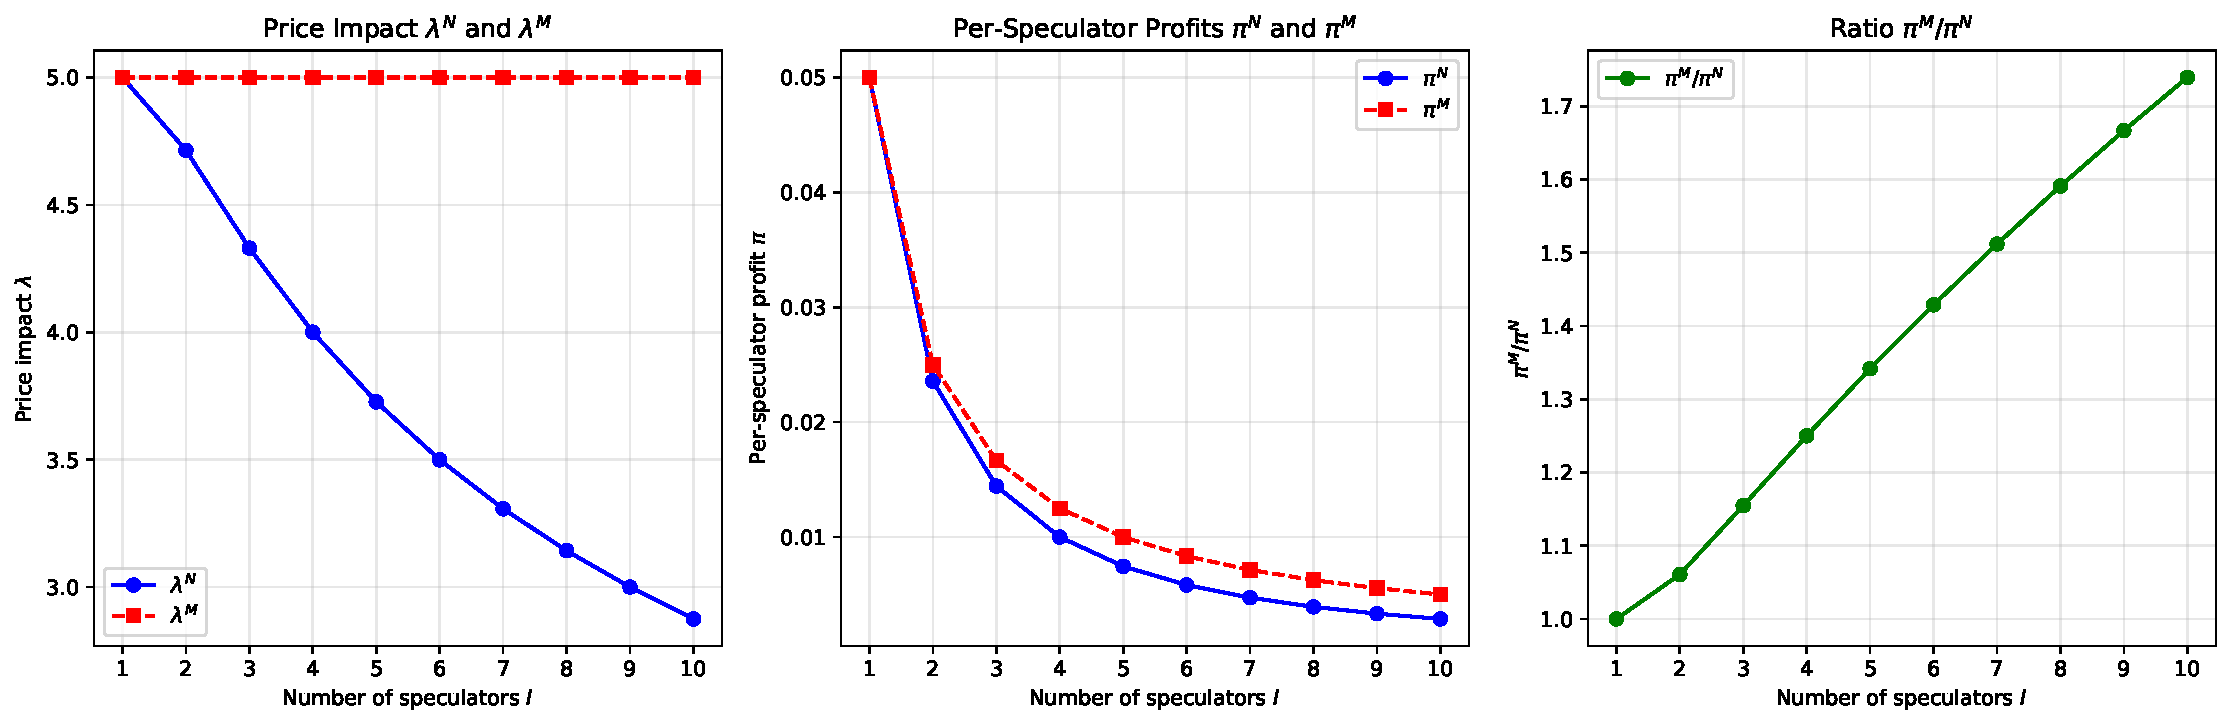
\includegraphics[width=\textwidth]{lambda_pi_ratio_plots.pdf}
    \caption{Price impact $\lambda$, per-speculator profits $\pi$, and profit ratio 
    $\pi^M/\pi^N$ under Nash and cartel equilibria, as functions of the number of 
    speculators $I$, for $\xi=0$, $\sigma_v=1$, $\sigma_u=0.1$.}
    \label{fig:lambda_pi_ratio}
\end{figure}

The plots show that $\lambda^M$ is constant in $I$ while $\lambda^N$ decreases, 
reflecting the fact that competition among Nash speculators reduces price impact, whereas 
the cartel maintains a fixed level of market illiquidity regardless of group size. Both 
$\pi^N$ and $\pi^M$ decrease in $I$, as the per-speculator share of total profits 
diminishes with more participants. However, $\pi^N$ falls strictly faster than $\pi^M$: 
in the Nash equilibrium, each speculator cannot coordinate to avoid the competition 
effect, so increasing $I$ undermines individual profits through the price impact of rivals. 
The cartel internalizes this competition effect, limiting total order 
flow and preserving profit margins more effectively. As a result, the ratio $\pi^M/\pi^N$ 
is strictly increasing in $I$, confirming that the incentive to collude grows with the 
number of speculators: the larger the group, the greater the gain from coordination 
relative to competitive trading.

\section{Market Quality}
Market quality refers to how well a financial market fulfills its main functions: 
incorporating information into prices, enabling trade at low cost, and limiting the 
exploitation of uninformed participants. In this model, noise traders represent 
liquidity traders, investors who trade for reasons unrelated to the fundamental 
value $v_t$, such as portfolio rebalancing or hedging needs. We measure market quality through three indicators:
\begin{itemize}
    \item \textbf{Price informativeness:} $\mathcal{I}=\frac{1}{\text{Var}(v_t\mid p_t)}=\frac{I^2\chi^2\sigma_v^2+\sigma_u^2}{\sigma_v^2\sigma_u^2}$, which measures how accurately the market price reflects the fundamental value $v_t$. A higher $\mathcal{I}$ indicates that prices are more informative.
    \item \textbf{Market liquidity:} $\mathcal{L}=\frac{1}{\lambda}$, which measures how cheaply traders can execute orders without moving prices. A higher $\mathcal{L}$ indicates a more liquid market.
    \item \textbf{Noise-trader losses:} $W_N=\lambda \sigma_u^2$, which measures the average losses incurred by noise traders due to adverse selection.
\end{itemize}

For $\xi=0$, we see from (\ref{lambda_N}) that as $I$ increases, $\lambda^N$ decreases 
(strictly for $I\ge 2$), since if we define $f(I)=\frac{\sqrt{I}}{I+1}$:
\[
f'(I)=\frac{\frac{1}{2\sqrt{I}}(I+1)-\sqrt{I}}{(I+1)^2}=\frac{-I+1}{2\sqrt{I}(I+1)^2}<0\quad \text{for }I\ge 2,
\]
and $f'(1)=0$.
The price informativeness in the Nash equilibrium is obtained by substituting 
$\chi^N = \frac{\sigma_u}{\sqrt{I}\sigma_v}$ into the expression for $\mathcal{I}$:
\[
\mathcal{I}^N=\frac{I^2(\chi^N)^2\sigma_v^2+\sigma_u^2}{\sigma_v^2\sigma_u^2}=
\frac{I^2\cdot\frac{\sigma_u^2}{I\sigma_v^2}\cdot\sigma_v^2+\sigma_u^2}{\sigma_v^2\sigma_u^2}=
\frac{I\sigma_u^2+\sigma_u^2}{\sigma_v^2\sigma_u^2}=\frac{I+1}{\sigma_v^2},
\]
which is strictly increasing in $I$ for all $I\ge 1$. The noise-trader losses in the
Nash equilibrium are
\[
W_N^N=\lambda^N\sigma_u^2=\frac{\sqrt{I}\sigma_v}{(I+1)\sigma_u}\cdot\sigma_u^2=
\sigma_u\sigma_v\cdot f(I),
\]
which is decreasing in $I$ (strictly for $I\ge 2$) by the same argument as for $\lambda^N$.

Substituting $\chi^M = \frac{\sigma_u}{I\sigma_v}$ into the same expressions gives
\[
\mathcal{I}^M = \frac{2}{\sigma_v^2}, \qquad W_N^M = \frac{\sigma_u\sigma_v}{2},
\]
both constant in $I$. The cartel therefore locks in a fixed level of price opacity 
and noise-trader exploitation regardless of group size, while the Nash equilibrium 
delivers progressively higher liquidity, more informative prices, and lower 
noise-trader losses as $I$ grows.

To illustrate these results numerically, a Python script computes $\lambda^N$, 
$\lambda^M$, $\mathcal{I}^N$, $\mathcal{I}^M$, $W_N^N$, and $W_N^M$ for $\xi=0$, 
$\sigma_v=1$, $\sigma_u=0.1$, and $I=1,2,\ldots,10$. Figure \ref{fig:market_quality} 
displays the resulting plots.

\begin{figure}[H]
    \centering
    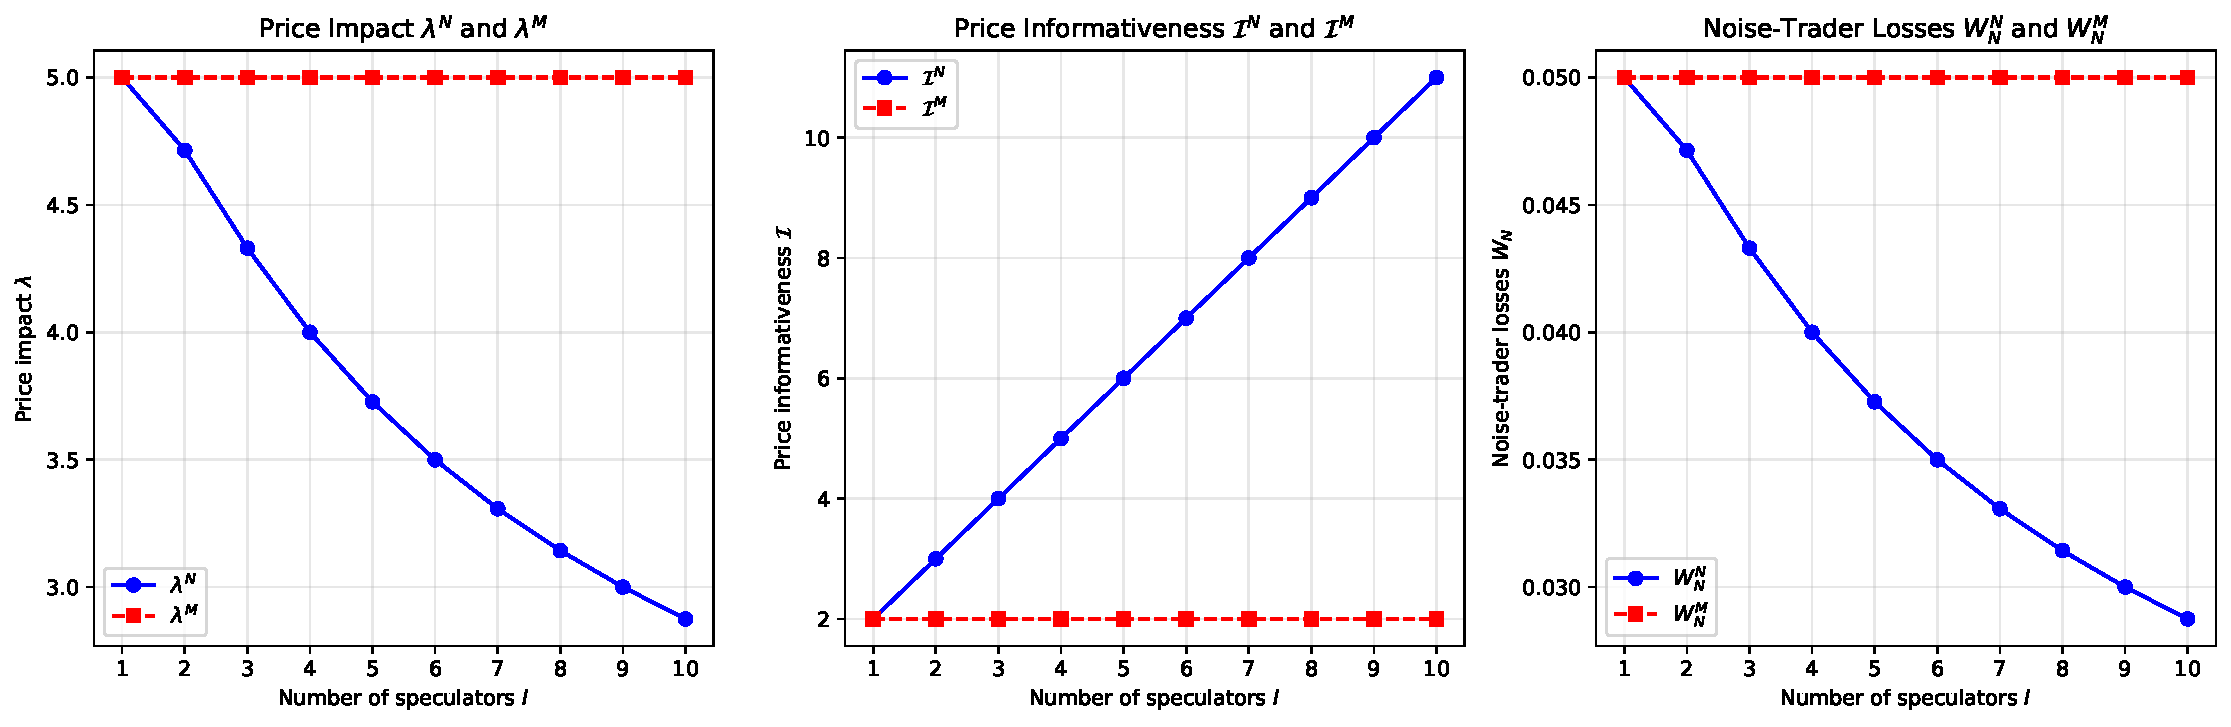
\includegraphics[width=\textwidth]{market_quality_plots.pdf}
    \caption{Price impact $\lambda$, price informativeness $\mathcal{I}$, and 
    noise-trader losses $W_N$ under Nash and cartel equilibria, as functions of 
    the number of speculators $I$, for $\xi=0$, $\sigma_v=1$, $\sigma_u=0.1$.}
    \label{fig:market_quality}
\end{figure}

The economic interpretation of the figure is the following: the constancy of the cartel 
curves reflects that the aggregate response coefficient $I\chi^M = \sigma_u/\sigma_v$ 
is independent of group size: the cartel simply divides a fixed monopolist trading 
volume equally among its members. Competition, by contrast, drives each Nash 
speculator to trade more strongly on their signal, increasing the informational 
content of total order flow relative to noise. The result is a strict welfare 
ranking: for every $I \geq 2$, the Nash equilibrium delivers lower price impact, 
more informative prices, and smaller noise-trader losses than the cartel, and the 
gap widens as $I$ grows. This confirms within the \citet{Dou2025} framework the 
result of \citet{Subrahmanyam1991} that competition among risk-neutral informed 
traders monotonically improves market quality (Lemma 2(i)).

For $\xi > 0$, the equilibrium quantities $\chi^N$, $\lambda^N$, $\chi^M$, and $\lambda^M$ 
cannot be solved in closed form\label{par:numerical_solver} and must instead be obtained numerically as the solution 
to a fixed-point problem. Specifically, the Nash equilibrium conditions in equations (4), (5), and (7) can be reduced to 
finding the root of:
\[
F(\chi) = \chi - \frac{1}{(I+1)\lambda(\gamma(\chi))}, \quad \text{where} \quad 
\gamma(\chi) = \frac{I\chi}{(I\chi)^2 + (\sigma_u/\sigma_v)^2}, \quad 
\lambda(\gamma) = \frac{\theta\gamma + \xi}{\theta + \xi^2},
\]
and analogously for the cartel, replacing $(I+1)$ with $2I$. A Python script was 
implemented to find these roots using Brent's method, which is a robust bracketing 
algorithm that combines bisection, secant, and inverse quadratic interpolation. The 
bracketing interval $[a, b]$ is determined automatically by expanding the upper bound 
geometrically until a sign change is detected, which is necessary since for large $\xi$ 
the equilibrium $\chi$ can be very large. The $\xi = 0$ case was used as a sanity check: 
the numerical results match the closed-form expressions derived in Section~3 exactly.

Table \ref{tab:numerical} reports the computed equilibrium quantities for $I=2$, 
$\sigma_v=1$, $\sigma_u=0.1$, $\theta=0.1$, and $\xi \in \{0, 50, 500\}$.

\begin{table}[H]
\centering
\begin{tabular}{ccccccc}
\toprule
$\xi$ & $\chi^N$ & $\lambda^N$ & $\pi^N$ & $\chi^M$ & $\lambda^M$ & $\pi^M$ \\
\midrule
$0$   & $0.0707$ & $4.7140$ & $0.0236$ & $0.0500$ & $5.0000$ & $0.0250$ \\
$50$  & $16.6663$ & $0.0200$ & $5.5554$ & $12.4995$ & $0.0200$ & $6.2498$ \\
$500$ & $166.6666$ & $0.0020$ & $55.5555$ & $125.0000$ & $0.0020$ & $62.5000$ \\
\bottomrule
\end{tabular}
\caption{Nash and cartel equilibrium quantities for $I=2$, $\sigma_v=1$, 
$\sigma_u=0.1$, $\theta=0.1$, and $\xi \in \{0, 50, 500\}$.}
\label{tab:numerical}
\end{table}

The results show that $\xi$ has a dramatic effect on equilibrium behavior. 
As $\xi$ increases, trading intensities $\chi^N$ and $\chi^M$ grow roughly in 
proportion to $\xi$, while price impact $\lambda^N$ and $\lambda^M$ go toward 
zero. The mechanism works as follows: large $\xi$ means information-insensitive 
investors absorb most of the order flow, so the market maker's pricing rule becomes insensitive to informed trading, allowing speculators to trade aggressively at little cost. Profits consequently grow by several orders of magnitude relative 
to the $\xi=0$ case. The absolute gap between $\pi^M$ and $\pi^N$ widens with $\xi$, 
indicating that information-insensitive investors amplify the gains from collusion. 
Nevertheless, the cartel always outperforms the Nash equilibrium ($\pi^M > \pi^N$) 
across all values of $\xi$, confirming that the incentive to collude persists 
regardless of the presence of information-insensitive investors.

Using the previous numerical solver, we compute $\lambda^N$, 
$\lambda^M$, $\mathcal{I}^N$, $\mathcal{I}^M$, $W_N^N$, and $W_N^M$ for $\xi=500$, 
$\theta=0.1$, $\sigma_v=1$, $\sigma_u=0.1$, and $I=1,2,\ldots,10$. The results are 
displayed in Figure \ref{fig:comp_statics_xi500}.

\begin{figure}[H]
    \centering
    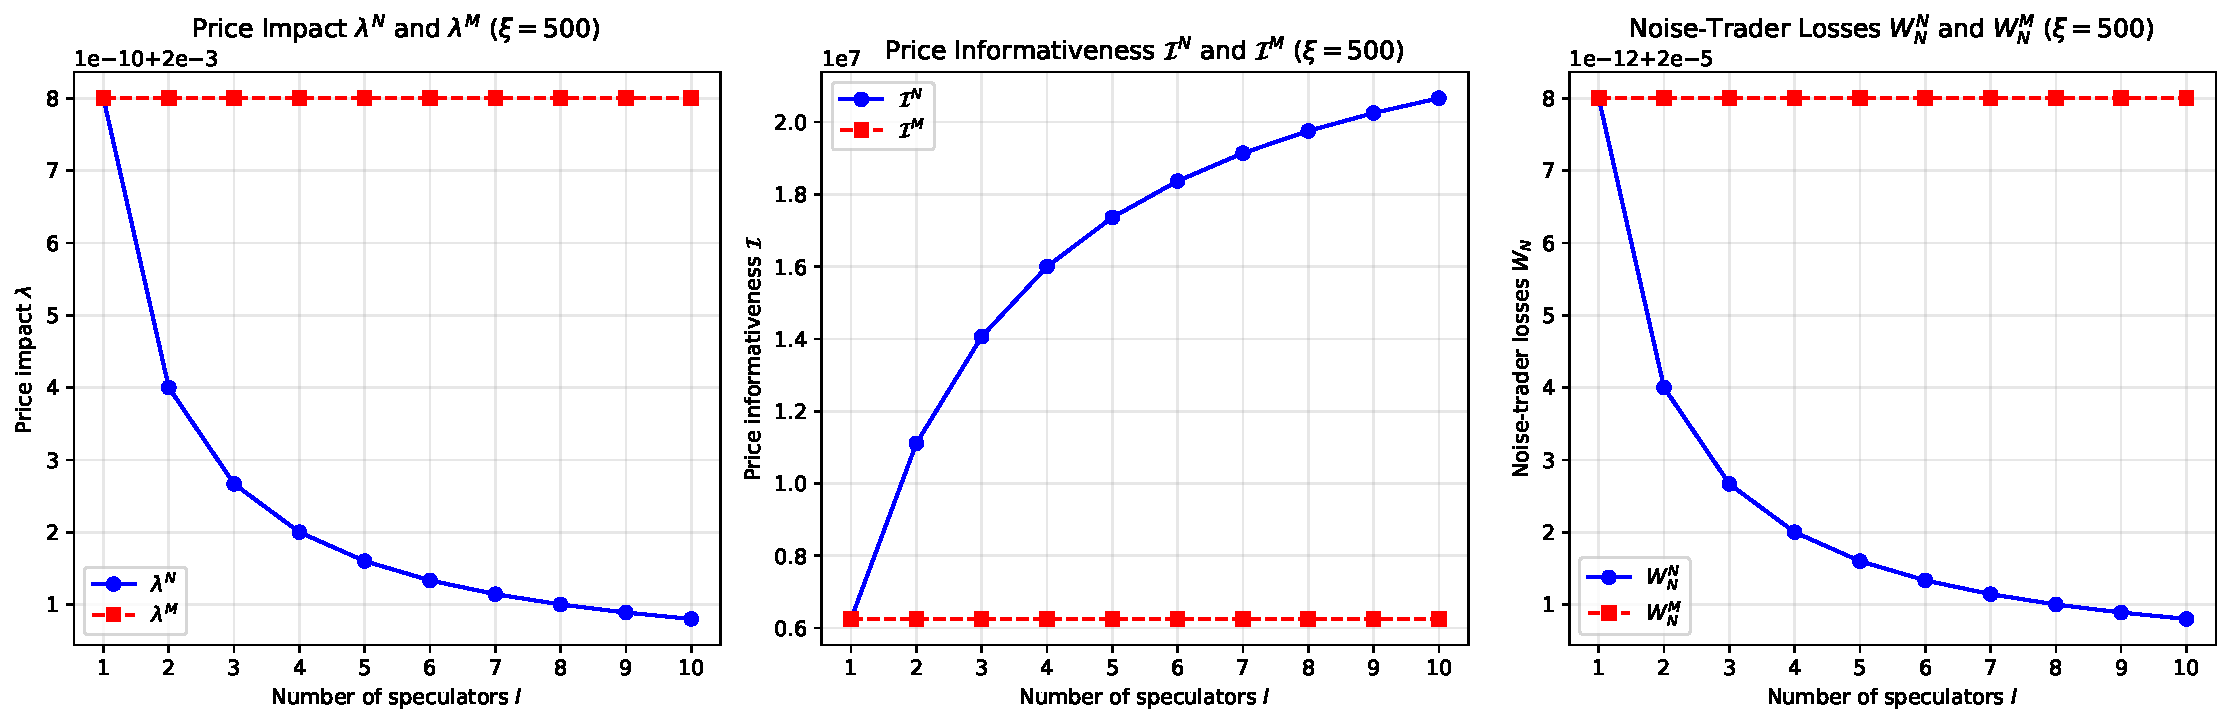
\includegraphics[width=\textwidth]{comparative_statics_xi500.pdf}
    \caption{Price impact $\lambda$, price informativeness $\mathcal{I}$, and 
    noise-trader losses $W_N$ under Nash and cartel equilibria as functions of 
    the number of speculators $I$, for $\xi=500$, $\theta=0.1$, $\sigma_v=1$, 
    $\sigma_u=0.1$.}
    \label{fig:comp_statics_xi500}
\end{figure}

Both $\lambda^N$
and $\lambda^M$ are of order $0.002$ at $\xi=500$ versus order $5$ at $\xi=0$, a
collapse of three orders of magnitude. The reason is that the pricing rule
$\lambda = (\theta\gamma + \xi) / (\theta + \xi^2)$ is dominated by the $\xi^2$ term
in the denominator for large $\xi$, giving $\lambda \approx 1/\xi = 0.002$. The
market maker becomes insensitive to information and prices primarily off the
liquidity parameter $\xi$, so insiders adjust $\chi$ but prices barely respond. The
left panel of Figure \ref{fig:comp_statics_xi500} shows $\lambda^N$ decreasing and
$\lambda^M$ flat, but the variations are of order $10^{-10}$ around a base of
$0.002$, both equal $0.002000$ to six decimal places for every $I$. The same
mechanism flattens noise-trader losses $W_N = \lambda \sigma_u^2$, which sit at
$2 \times 10^{-5}$ with variations of order $10^{-12}$.

The informativeness gap behaves differently. At $I=10$, the ratio
$\mathcal{I}^N/\mathcal{I}^M$ is roughly $3.3$ at $\xi=500$, against $5.5$ at
$\xi=0$: information-insensitive investors close part of the gap because the cartel also trades more harshly in this regime. In absolute terms, both $\mathcal{I}^N$ and $\mathcal{I}^M$ are orders of magnitude larger at $\xi=500$ than at $\xi=0$,
reflecting the much higher trading intensity of all speculators. The welfare ranking is the same: competition delivers substantially more informative prices than collusion, but the margin is smaller.

We now turn to a complementary way of quantifying the market impact of collusion: 
the effective number of insiders $I^*$, defined as the value such that 
$\lambda^N(I^*) = \lambda^M(I)$. That is, $I^*$ is the number of Nash speculators 
needed to replicate the price impact of a cartel with $I$ speculators. For $\xi=0$, 
using the closed-form expressions for $\lambda^N$ and $\lambda^M$:
\[
\lambda^N(I^*) = \frac{\sqrt{I^*}\,\sigma_v}{(I^*+1)\sigma_u}, \qquad 
\lambda^M(I) = \frac{\sigma_v}{2\sigma_u}.
\]
Setting these equal and canceling $\sigma_v/\sigma_u$ (note that $\lambda^M$ doesn't depend on $I$):
\[
\frac{\sqrt{I^*}}{I^*+1} = \frac{1}{2} \iff 2\sqrt{I^*} = I^*+1 \iff 
4I^* = (I^*+1)^2 \iff I^{*2} - 2I^* + 1 = 0 \iff (I^*-1)^2 = 0,
\]
which has the unique solution $I^*=1$, regardless of $I$, $\sigma_v$, and $\sigma_u$.
This means that a cartel of $I$ speculators generates exactly the same price impact 
as a Nash equilibrium with a single speculator, i.e. a monopolist. The cartel therefore 
trades as conservatively as a monopolist regardless of its size, which makes 
intuitive sense: the cartel maximizes joint profits, and adding more members to the cartel does not change its 
aggregate trading behavior, it simply divides the same monopolist trading volume among more participants.

We now extend the analysis to $\xi=500$, where closed-form expressions are no
longer available. For each $I \in \{2, 3, 5\}$ we compute $\lambda^M(I)$ using
the equilibrium solver and find $I^*$ such that $\lambda^N(I^*) = \lambda^M(I)$
via Brent's method, treating $I^*$ as the unknown. Uniqueness on the
interval $[0.01, 10]$ is verified by a sign-change check on a $2{,}000$-point
grid.

For $\theta=0.1$, $\sigma_v=1$, $\sigma_u=0.1$, the solver returns $I^* = 1$ in
all three cases, with a unique solution each time. This is the same answer as
at $\xi = 0$, and it is not an accident: the cartel FOC $\chi^M = 1/(2I\lambda^M)$
implies that the aggregate cartel coefficient $I\chi^M$ depends only on $\lambda^M$,
which makes $\gamma^M$ and hence $\lambda^M$ constant in $I$. Combined with the
identity $\lambda^N(1) = \lambda^M(1)$, this gives $\lambda^N(1) = \lambda^M(I)$ for every
$I$, so $I^* = 1$ exactly.

Thus, the role of information-insensitive investors is not to change the fact that a cartel of any size trades like a monopolist; it is to
compress the level of price impact at which it happens. At $\xi = 0$,
$\lambda^N(1) = \lambda^M(I) = \sigma_v/(2\sigma_u) = 5$. At $\xi = 500$, the
common value collapses to $\lambda \approx 1/\xi = 2 \times 10^{-3}$, three orders
of magnitude smaller. Information-insensitive investors moderate the market impact of collusion (prices barely respond to informed order flow
in either equilibrium) without altering the equivalence between the
cartel and a monopolist.



\section{Q-Learning and Algorithmic Collusion}

\subsection{Algorithm Description}

We investigate whether model-free Q-learning algorithms, acting as informed
speculators, can learn to collude without explicit communication. The
simulation setup follows \citet{Dou2025}: each speculator $i$ maintains a
Q-matrix $\hat{Q}_i(s, x)$ indexed by state $s = (p_{t-1}, v_{t-1}, v_t)$
and action $x$, chooses actions via $\varepsilon$-greedy exploration with
state-dependent exploration rate $\varepsilon_t(v_k) = e^{-\beta\, t(v_k)}$,
and updates its Q-matrix according to
\begin{equation}
    \hat{Q}_{i,t+1}(s_t, x_{i,t}) = (1-\alpha)\,\hat{Q}_{i,t}(s_t, x_{i,t}) +
    \alpha\left[\pi_{i,t} + \rho \max_{x'}\hat{Q}_{i,t}(s_{t+1}, x')\right],
    \label{eq:Qupdate}
\end{equation}
with the max taken over the action grid corresponding to $v_{t+1}$. All
other entries remain unchanged. We use $n_v = 10$ value
grid points, state-dependent action grids of size $n_x = 15$ and price
grids of size $n_p = 31$, with bracketing parameter $\iota = 0.1$. Lagged
prices $p_{t-1}$ are discretised on the price grid corresponding to
$v_{t-1}$, since they were generated by actions chosen for that value
state. The Q-matrix is initialised as
\begin{equation}
    \hat{Q}_{i,0}(s, x_n) = \frac{1}{(1-\rho)\,n_x} \sum_{x_{-i} \in \mathcal{X}_k}
    \left[v_k - \left(\bar{v} + \lambda^N(x_n + (I-1)x_{-i})\right)\right] x_n,
    \label{eq:Qinit}
\end{equation}
which is the discounted payoff to speculator $i$ if the other speculators
randomise uniformly and the noise trader's order is zero, replicated
across all $(v_{t-1}, p_{t-1})$ slices.

The degree of collusion is measured by
\begin{equation}
    \Delta_\chi = \frac{\chi^N - \bar{\chi}^C}{\chi^N - \chi^M},
    \label{eq:collusion_index}
\end{equation}
where $\bar{\chi}^C$ is the average learned trading intensity:
$\Delta_\chi = 0$ corresponds to Nash, $\Delta_\chi = 1$ to perfect
cartel. Throughout, we use $\bar{v} = 1$, $\sigma_v = 1$, $\sigma_u = 0.1$,
$I = 2$, $\rho = 0.95$, $\theta = 0.1$, $\alpha = 0.05$,
$\beta = 5 \times 10^{-6}$. The discretisation grids depend on $\chi^N$,
$\chi^M$, and $\lambda^N$ and are recomputed for each value of $\xi$.

\subsection{Simulation Results}
As a baseline sanity check we ran $I=1$, where $\chi^N=\chi^M=\sigma_u/\sigma_v=0.1$ 
and the action grid collapses to a single point at every value-grid node 
($x_k^N=x_k^M$). The simulation returns $\bar\chi^C=0.100000$, matching the 
closed form exactly.

This should be interpreted as a consistency check rather than evidence 
of non-trivial strategic learning. When $I=1$, the Nash and cartel order sizes 
are identical at every value-grid point, so the prescribed action-grid 
construction becomes degenerate: the interval $[x_k^M - \iota(x_k^N - x_k^M),\ 
x_k^N + \iota(x_k^N - x_k^M)]$ collapses to a single point when $x_k^N = x_k^M$, 
making every action on the grid identical. The test confirms that the discretization, state transitions, market-clearing step, and Q-learning updates are implemented coherently.

We now turn to the more interesting case of $I=2$ informed speculators,
where $\chi^N \neq \chi^M$ and the Q-learning algorithm must make a
choice between the high Nash intensity and the conservative cartel
intensity. The closed-form benchmarks at $\xi=0$, $I=2$ are
$\chi^N = \sigma_u/(\sqrt{2}\sigma_v) \approx 0.0707$,
$\chi^M = \sigma_u/(2\sigma_v) = 0.05$, and
$\lambda^N = \sqrt{2}\sigma_v/(3\sigma_u) \approx 4.714$. The action grid is now
non-degenerate, spanning trading intensities that allow speculators to deviate
below the cartel level or above the Nash level by a factor of $\iota = 0.1$.

\paragraph{Implementation choice: three update protocols.}
The protocol can be read in more than one way: each speculator maintains a
Q-matrix $\hat{Q}_i(s,x)$ (with subscript $i$), yet the speculators are also
described as sharing the same Q-matrix and update rule. We compare three variants:
\begin{itemize}
    \item \textbf{Separate matrices.} Each speculator $i \in \{1, 2\}$
    maintains its own Q-matrix $\hat{Q}_i$, identically initialized via
    Eq.~(\ref{eq:Qinit}) and updated only by its own experience according to
    Eq.~(\ref{eq:Qupdate}). Symmetry between agents emerges endogenously
    from identical dynamics rather than from enforcing a single shared matrix.
    This is the obvious interpretation and what the paper uses.
    \item \textbf{Shared matrix, sequential updates.} A single Q-matrix is
    consulted by both agents. Each period, both agents' updates are applied
    to that matrix in sequence. When both agents happen to pick the same
    $(\text{state}, \text{action})$ cell in the same period, the second update
    operates on the value already modified by the first, introducing a
    path-dependence.
    \item \textbf{Shared matrix, averaged updates.} A single Q-matrix is again
    used. Targets are computed per agent and grouped by the cell they would
    update. When multiple agents hit the same cell, their targets are averaged
    before a single update is applied, making the update order-independent and
    symmetric across agents.
\end{itemize}
The separate-matrices variant is our primary specification; the two
shared-matrix variants serve as a robustness check on whether the collusive
outcome is an artifact of any particular update protocol.

We measure convergence of the learned greedy policy rather than of the
Q-values, which fluctuate at the constant rate $\alpha = 0.05$. The original paper requires every cell's greedy action to remain unchanged for $10^6$ consecutive
periods, a criterion calibrated for their ensemble of $1{,}000$ sessions of
length $2 \times 10^7$ to $5 \times 10^{10}$. This is too strict for our
single-session simulations, so we adopt a softer per-cell variant: at each
diagnostic checkpoint, we report the fraction of $(s, i)$ cells whose greedy
action has been unchanged for at least $10^6$ consecutive periods. Combined
with the trajectory of $\bar{\chi}^C$, this provides a quantitative summary
of policy stationarity.

Our initial runs at $T = 50 \times 10^6$ training periods revealed that under all three
protocols the greedy policy was still drifting: the $\bar{\chi}^C$
trajectory was visibly trending downward, and the fraction of cells
stable for at least $10^6$ consecutive periods sat between roughly $10\%$
and $20\%$, indicating that most of the policy was still changing.
To obtain interpretable estimates we extend the training horizon to
$T = 500 \times 10^6$ periods.

\paragraph{Measurement of $\bar{\chi}^C$.}
For each variant we train the Q-learning algorithms for $T = 500 \times 10^6$
periods, freeze the Q-matrix or matrices, and evaluate the resulting greedy
policy over an additional $T_{\text{eval}} = 10^5$ periods with exploration
and learning both turned off. Following \citet[Internet Appendix,
eq.~(IA.4.4)]{Dou2025}, for each speculator $i$ we run the unrestricted OLS
regression
\[
x_{i,t} = \chi^C_{i,0} + \chi^C_{i,1}\,v_t + \epsilon_t
\]
over the $T_{\text{eval}}$ frozen-policy sample, and report
\[
\bar{\chi}^C = \frac{1}{I} \sum_{i=1}^{I} \hat{\chi}^C_{i,1}.
\]
This slope-based estimator is numerically more stable than the per-period
ratio $x_{i,t}/(v_t - \bar{v})$, which is sensitive to realisations of $v_t$
close to $\bar{v}$, and it directly tests whether the learned policy takes
the theoretically-motivated linear form in $(v_t - \bar{v})$.

\paragraph{Results.}
Table~\ref{tab:irf_methods} summarises the three runs. All three protocols
yield substantial collusion, with $\Delta_\chi \in [0.72, 0.92]$, and the
ordering is
$\Delta_\chi^{\text{separate}} < \Delta_\chi^{\text{averaged}}
< \Delta_\chi^{\text{sequential}}$.

\begin{table}[H]
    \centering
    \begin{tabular}{lccc}
        \toprule
        Method & $\bar{\chi}^C$ & $\Delta_\chi$ &
        \begin{tabular}{c}Cells stable\\$\geq 10^6$ periods\end{tabular} \\
        \midrule
        Separate   & $0.0558$ & $0.720$ & $98.5\%$ \\
        Sequential & $0.0517$ & $0.919$ & $98.1\%$ \\
        Averaged   & $0.0520$ & $0.902$ & $98.4\%$ \\
        \bottomrule
    \end{tabular}
    \caption{Learned trading intensity and convergence diagnostic under the
    three update protocols at $\xi=0$, $I=2$, $T = 500 \times 10^6$. The
    ``cells stable'' column reports the fraction of $(s,i)$ cells whose
    greedy action has been unchanged for at least $10^6$ consecutive
    periods at the end of training.}
    \label{tab:irf_methods}
\end{table}

The $\bar{\chi}^C$ trajectories for all three methods stabilize during the
final $250 \times 10^6$ periods (fluctuations on the order of $10^{-4}$), so the OLS
estimates are reliable. The per-cell stability metric reaches near $98\%$,
with $1$-$2\%$ of cells showing ongoing argmax oscillation due to
near-tied Q-values across adjacent cells; this would
likely be eliminated under \citet{Dou2025}'s smaller learning rate
$\alpha = 0.01$, but does not affect our conclusions.

Across all three protocols, the algorithms learn to trade well
below the Nash intensity and capture between approximately $0.7$ and $0.9$ of
the distance toward the perfect cartel. This shows that the
collusive outcome is not an artifact of any particular method, but a feature of Q-learning in this setting. The
collusive outcome arises without any communication or shared information beyond the Q-learning update rule.

The separate matrices method results in a noticeably lower $\Delta_\chi$
than the two shared matrix protocols ($0.72$ versus $0.90$-$0.92$). Since the stability is essentially identical ($\sim 98\%$) and
$\bar{\chi}^C$ has stabilized in all three cases, this gap reflects a
genuine difference in the learned equilibrium rather than a convergence
feature. A natural explanation is that shared protocols apply two
updates per cell per period (either sequential or
averaged), which effectively doubles the learning rate at cells the two
agents both visit. Faster Q-value separation then causes the argmax to
commit more to the action that first gets an advantage during
the exploration phase. If that action is conservative,
the shared protocols over-prune more effectively and land closer to
the cartel.

Moreover, our results are based on single simulation sessions, whereas \citet{Dou2025}
report ensemble averages across $1{,}000$ independent sessions. Given the
paper's observation that individual sessions can converge to different
equilibria due to randomness in exploration, our reported $\Delta_\chi$
values should be interpreted as point estimates with non-trivial variance. A more comprehensive analysis would
average across multiple independent runs per protocol. \\

We now consider the regime $\xi = 500$, in which a substantial mass of
information-insensitive investors absorbs informed order flow at prices
close to $\bar{v}$. Since closed-form expressions are no longer available,
we solve the fixed-point system from Section~\ref{par:numerical_solver} numerically using
Brent's method and obtain
\[
\chi^N \approx 166.667, \qquad \chi^M = 125.000, \qquad
\lambda^N \approx 2.000 \times 10^{-3},
\]
which differ from the $\xi=0$ benchmarks by roughly three orders of
magnitude. The intuition is that information-insensitive
investors provide an additional channel of liquidity beyond the noise
trader, collapsing $\lambda^N$ and allowing informed speculators to
trade much more aggressively in absolute terms while preserving the
per-unit margin $v_t - p_t$. The action and price grids are rebuilt
with these new equilibrium values. We run each of the three update protocols
for the horizon $T = 500 \times 10^6$ periods, and
evaluate the frozen greedy policy over $T_{\text{eval}} = 10^5$
additional periods using the same OLS estimator
$\bar{\chi}^C = I^{-1}\sum_i \hat{\chi}^C_{i,1}$ as before.

\paragraph{Results.}
Table~\ref{tab:xi500} summarizes the three runs.

\begin{table}[H]
    \centering
    \begin{tabular}{lccc}
        \toprule
        Method & $\bar{\chi}^C$ & $\Delta_\chi$ &
        \begin{tabular}{c}Cells stable\\$\geq 10^6$ periods\end{tabular} \\
        \midrule
        Separate   & $153.80$ & $0.309$ & $96.5\%$ \\
        Sequential & $130.60$ & $0.866$ & $98.1\%$ \\
        Averaged   & $130.65$ & $0.865$ & $97.5\%$ \\
        \bottomrule
    \end{tabular}
    \caption{Learned trading intensity and convergence diagnostic under
    the three update protocols at $\xi=500$, $I=2$, $T = 500 \times 10^6$.
    Closed-form benchmarks: $\chi^N \approx 166.67$,
    $\chi^M = 125.00$.}
    \label{tab:xi500}
\end{table}

The $\bar{\chi}^C$ trajectories stabilise across all three protocols
during the second half of training, and the per-cell stability
plateaus near $96$-$98\%$, matching the patterns observed at $\xi=0$.
The two speculators in the separate-matrices run learn nearly identical
policies, so the gap with the
shared-Q protocols is again a genuine equilibrium effect.

Placing the two regimes side by side reveals a surprising pattern:

\begin{table}[H]
    \centering
    \begin{tabular}{lcc}
        \toprule
        Method & $\Delta_\chi^{\xi=0}$ & $\Delta_\chi^{\xi=500}$ \\
        \midrule
        Separate   & $0.720$ & $0.309$ \\
        Sequential & $0.919$ & $0.866$ \\
        Averaged   & $0.902$ & $0.865$ \\
        \bottomrule
    \end{tabular}
    \caption{Collusion index across regimes for the three update protocols.}
    \label{tab:xi_comparison}
\end{table}

The two shared-Q protocols deliver similar collusion in both regimes
($\Delta_\chi \approx 0.87$-$0.92$), while the separate-matrices protocol
drops sharply from $0.72$ at $\xi=0$ to $0.31$ at $\xi=500$. To verify that
this gap is not a session-level artifact, we re-ran the separate-matrices
protocol at $\xi=500$ with four additional random seeds. The five sessions
returned $\Delta_\chi$ values of $\{0.307, 0.306, 0.328, 0.315, 0.320\}$,
with mean $0.316$ and standard deviation $0.009$, giving a 95\% confidence
interval of $[0.308, 0.323]$. The per-cell stability metric exceeded
$92\%$ in every run. The collusion gap between separate-matrices and
shared-Q is therefore a genuine equilibrium difference between the
protocols, not a sampling artifact. The IRF analysis in the next section
disentangles the mechanisms underlying both regimes.

\subsection{Impulse Response Analysis}
\label{sec:irf}

The previous section showed that Q-learning algorithms converge to partially
collusive strategies ($\Delta_\chi > 0$) in both the $\xi = 0$ and $\xi = 500$
regimes. We now ask what sustains this collusion. The authors identify two
distinct mechanisms. The first, \emph{price-trigger strategies}, works through
implicit coordination: speculators monitor lagged prices and revert to
aggressive trading whenever a price movement looks like a deviation by a rival.
The second, \emph{over-pruning bias}, works through learning: aggressive
actions are punished more heavily by adverse noise-trading shocks during
training, so the algorithms systematically undervalue and prune them, ending up with a conservative policy regardless of any rival's behavior. Both
mechanisms produce similar levels of steady-state collusion, but their
signatures are different: price-trigger collusion reacts to an unexpected
price movement with a punishment phase, while over-pruning collusion does not react at all.

To distinguish between the two mechanisms empirically, we build a
noise shock impulse response function (IRF) following the protocol of
\citet[Section~5.3]{Dou2025}. After the Q-matrices have stabilized, we
freeze them and draw $N_{\text{sim}} = 1{,}000$ independent paths of
fundamental values $\{v_1, \ldots, v_H\}$ and noise realizations
$\{u_1, \ldots, u_H\}$ with horizon $H = 9$. Each path is simulated twice
under common random numbers: once as a baseline, and once with an
exogenous shock applied to the noise trader's order at $t = 3$,
$u_3 \leftarrow u_3 + u_{\text{shock}} \cdot \text{sgn}(v_3 - \bar{v})$,
directed in line with the informed speculators' trade. We use three shock
magnitudes calibrated as $0.5\%$, $2.5\%$, and $7\%$ of the average
absolute order size $\mathbb{E}[|x_i|]$ under the learned policy,
producing small, medium, and large price deviations at $t = 3$.

To aggregate responses across paths with different signs of
$v_t - \bar{v}$, we define the sign-adjusted variables
$\tilde{p}_t = (p_t - \bar{v}) \text{sgn}(v_t - \bar{v})$ and
$\tilde{x}_{i,t} = x_{i,t} \text{sgn}(v_t - \bar{v})$, which by
construction are positive in expectation. For each variable we average
across the $N_{\text{sim}}$ paths and report the percentage deviation of
the shocked average from the baseline (long-run) mean for price
$\tilde{p}_t$, per-speculator profit $\pi_t$, and order flow
$\tilde{x}_t$, at each horizon $t = 1, \ldots, 9$.

The two mechanisms predict very different IRF signatures. Under
price-trigger, an elevated $p_{t-1}$ is read as a sign of defection from cartel behavior, so
both speculators trade at $t = 4$ to punish the suspected deviator. If the trigger threshold is crossed, this
generates an order-flow response and an amplified price deviation at
$t = 4$ that can match or exceed the $t = 3$ spike
\citep[Figure~3]{Dou2025}. Under over-pruning, the learned policy is
essentially state-independent, so the shocked $p_3$ leaves the $t = 4$
actions unchanged and prices go back to baseline immediately
\citep[Figure~4]{Dou2025}.

We begin with $\xi = 0$. Across all three update protocols and all three
shock sizes, the IRFs show the same pattern. The price
spikes at $t = 3$ in proportion to the shock magnitude
($\approx 0.26\%$, $1.31\%$, and $3.66\%$ for the small, medium, and
large shocks respectively), and the per-speculator profit drops by
approximately the same percentage in absolute terms, reflecting the price-impact response $\Delta p_3 \approx \lambda^N
u_{\text{shock}}$. At $t = 4$ the price deviation is dampened in every
case, falling within $[-0.33\%, 0.20\%]$ across the three methods and
three shock sizes: between one and two orders of magnitude smaller than
the $t = 3$ spike, and with no consistent sign across methods. The
order-flow deviation at $t = 4$ stays within the same range. By
$t = 6$-$7$ all responses have decayed to noise-floor levels.

\begin{figure}[h!]
    \centering
    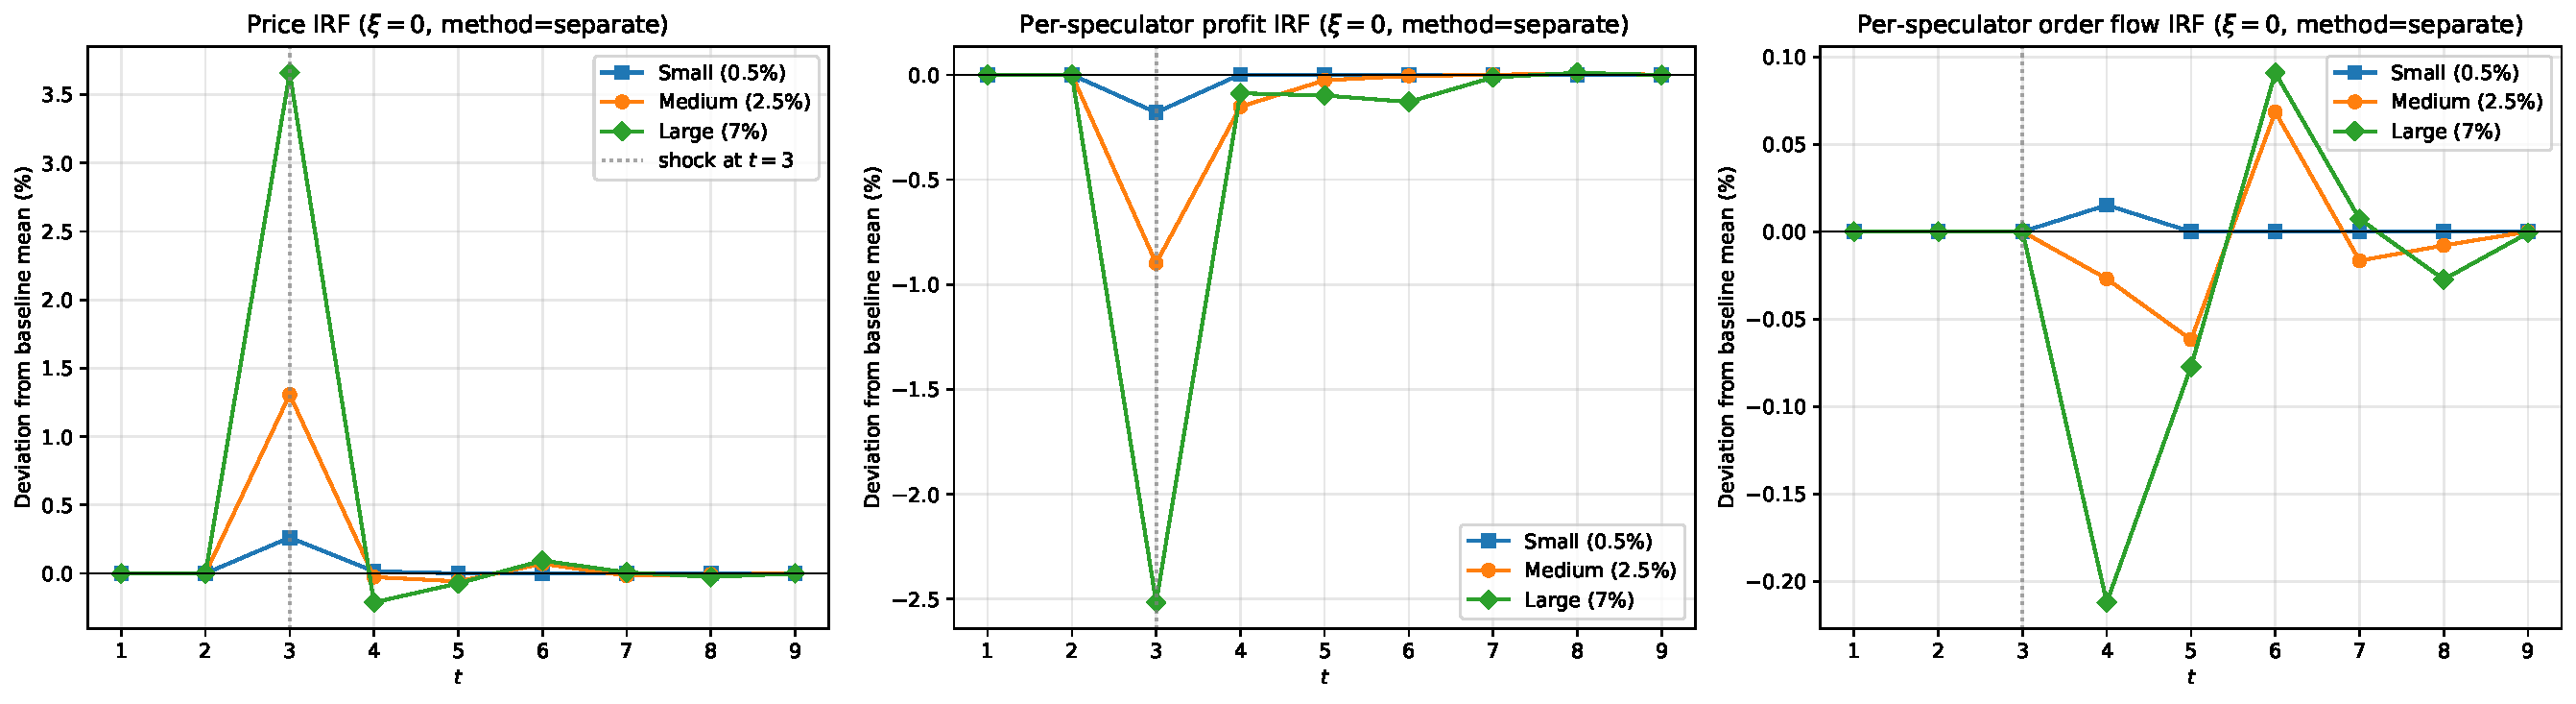
\includegraphics[width=0.85\textwidth]{irf_xi0_separate_I2.pdf}
    \\[0.5em]
    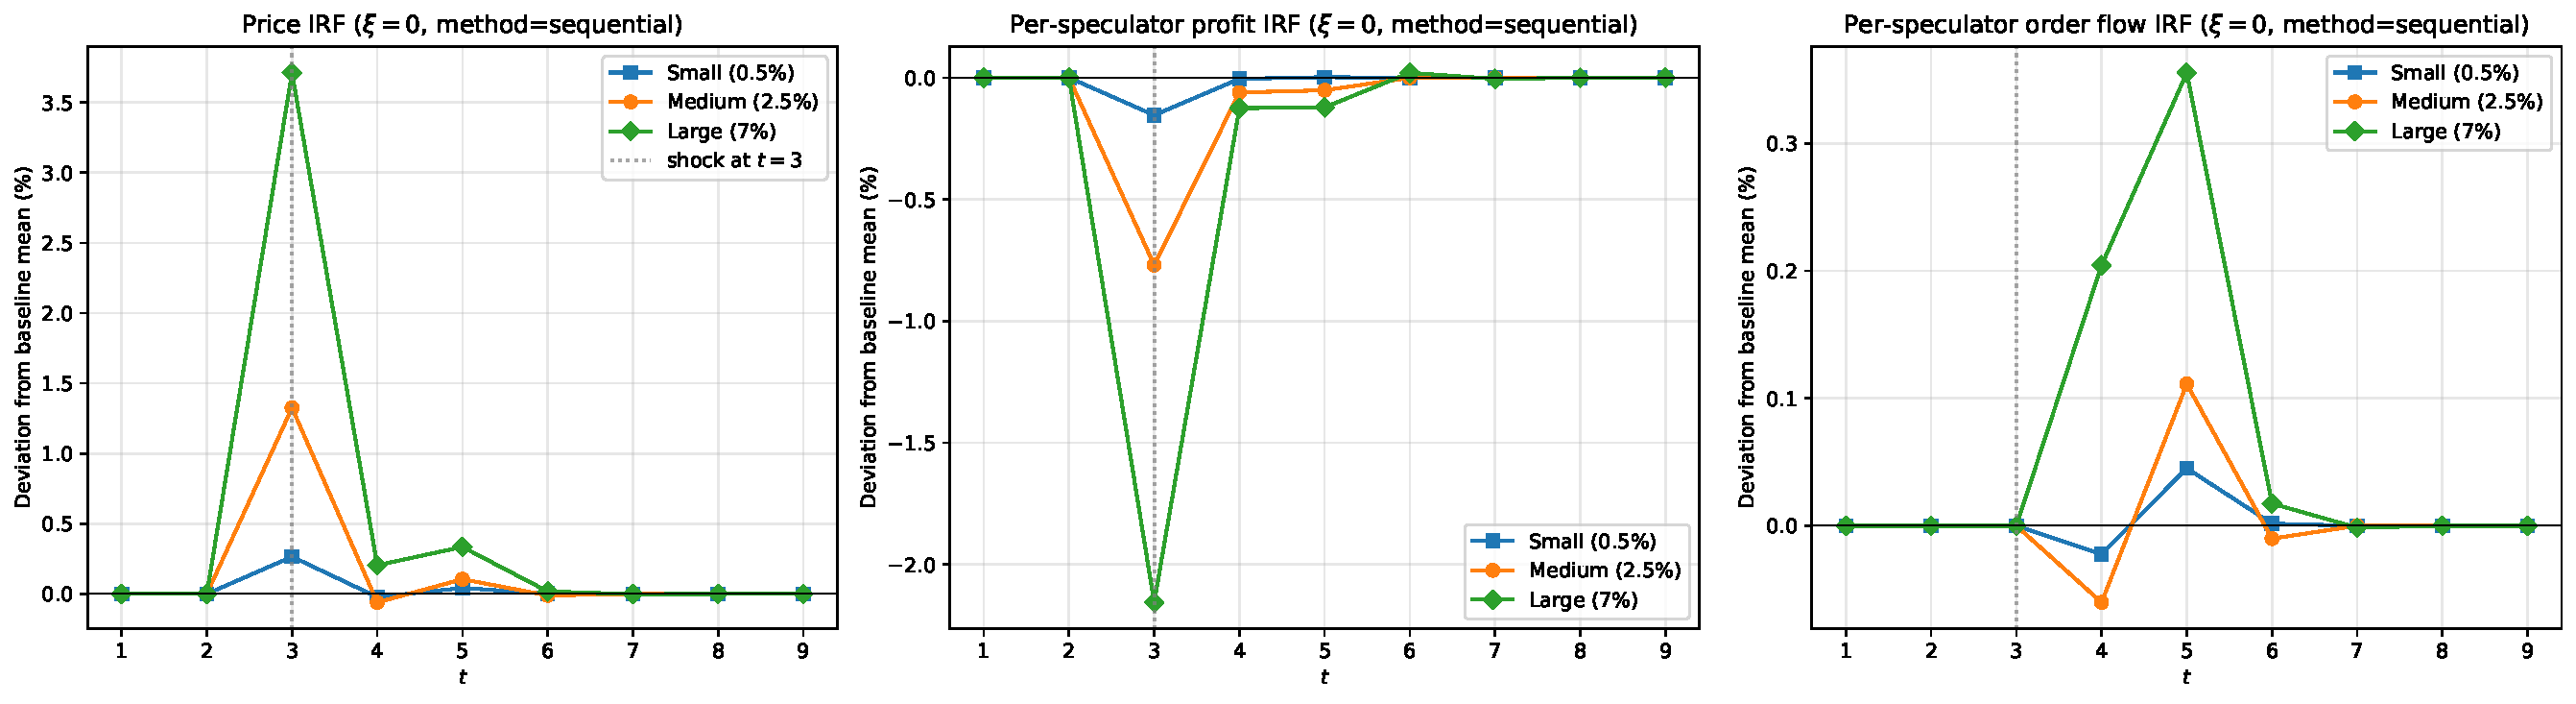
\includegraphics[width=0.85\textwidth]{irf_xi0_sequential_I2.pdf}
    \\[0.5em]
    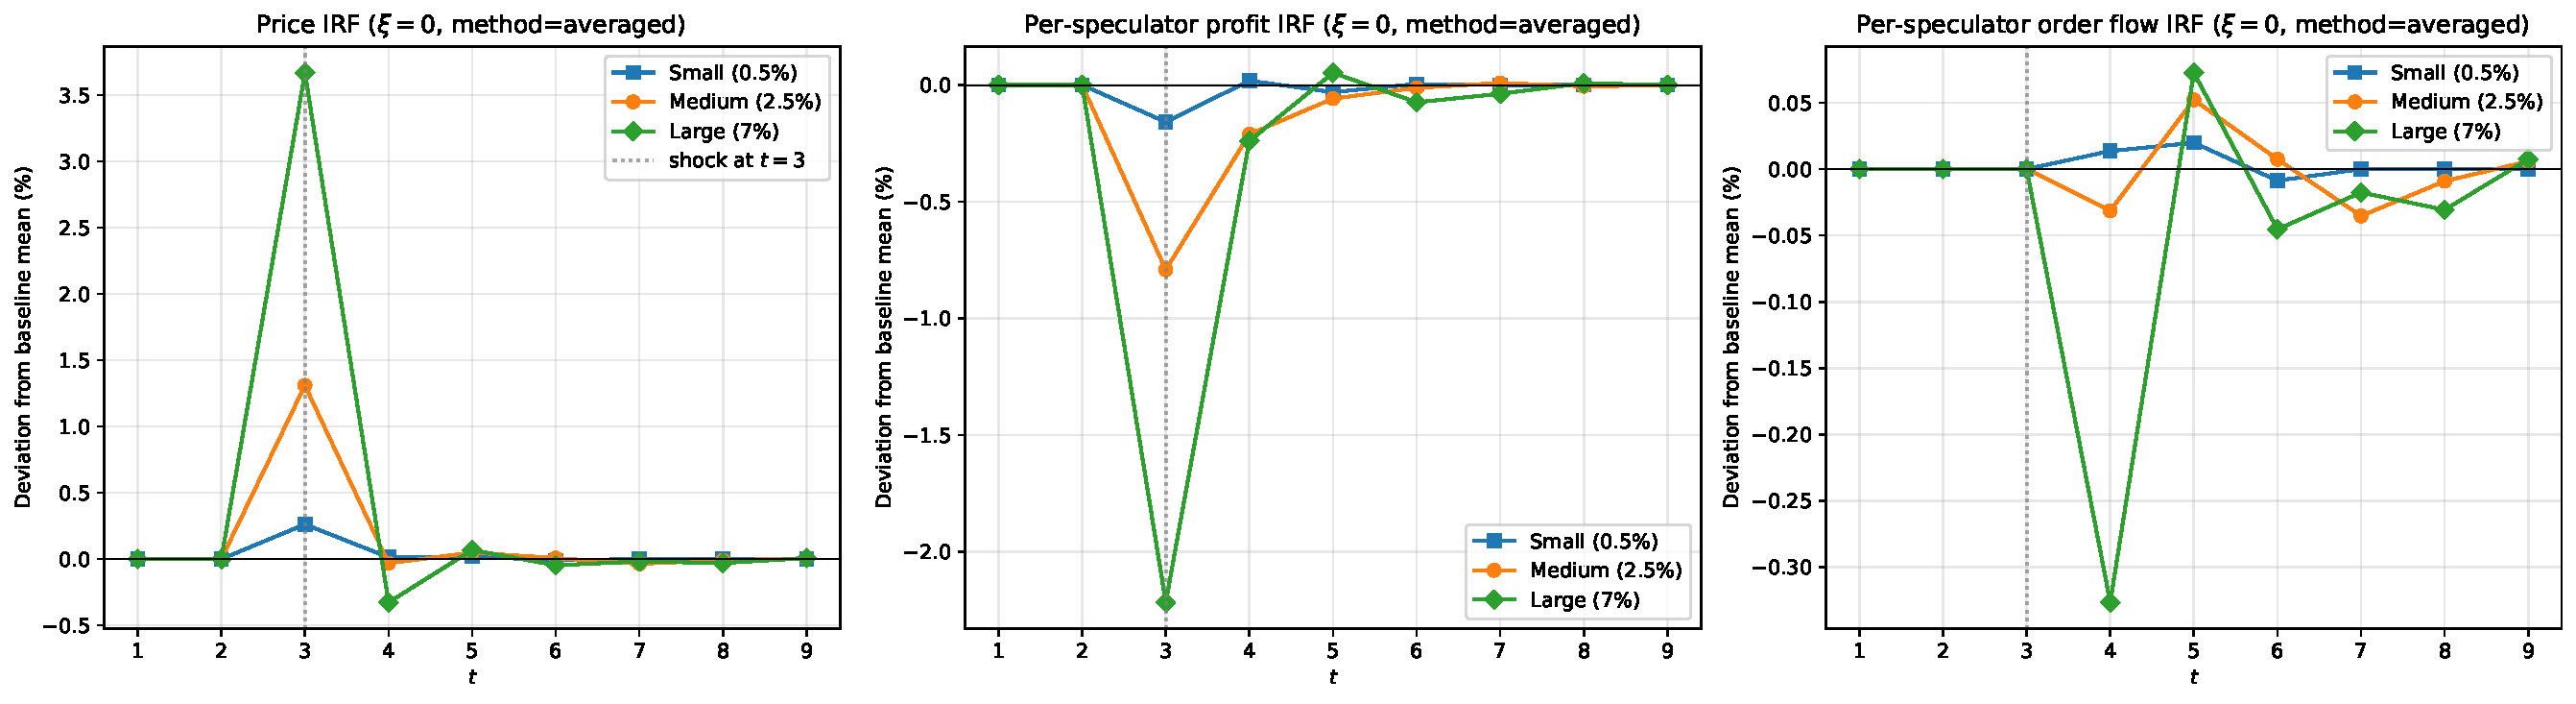
\includegraphics[width=0.85\textwidth]{irf_xi0_averaged_I2.pdf}
    \caption{Impulse response functions at $\xi = 0$ for the three update
    methods (top to bottom: separate, sequential, averaged). Across all
    panels, the response decays to zero immediately after the
    $t = 3$ spike.}
    \label{fig:irf_xi0}
\end{figure}

This pattern matches the over-pruning prediction: no order-flow
adjustment at $t = 4$ and dampening of price deviation. The
absence of any state-dependent response is exactly what the authors
predict for case (iii) of their taxonomy (low $\xi$, low $\sigma_u$),
where price-trigger strategies have no profitable foundation and
over-pruning is the only mechanism available \citep[Section~5.5]{Dou2025}.

The picture at $\xi = 500$ is somewhat different: the $t = 3$ spike is similar in proportional terms to the $\xi = 0$ case
($0.25\%$, $1.23\%$, $3.44\%$ across all methods), but the response at
$t = 4$ and beyond depends strongly on the update protocol. Under the
two shared protocols, both price and order flow exhibit large
positive deviations at $t = 4$, often exceeding the spike at $t = 3$.
The sequential medium shock, for example, yields $\tilde p_3 = 1.23\%$
followed by $\tilde p_4 = 4.40\%$, an amplification factor of $3.6$.
The $t = 4$ deviations approach a similar level
($\approx 4$-$5\%$) for medium and large shocks, while remaining $\approx 1$-$2\%$ for the small shock.

\begin{figure}[h!]
    \centering
    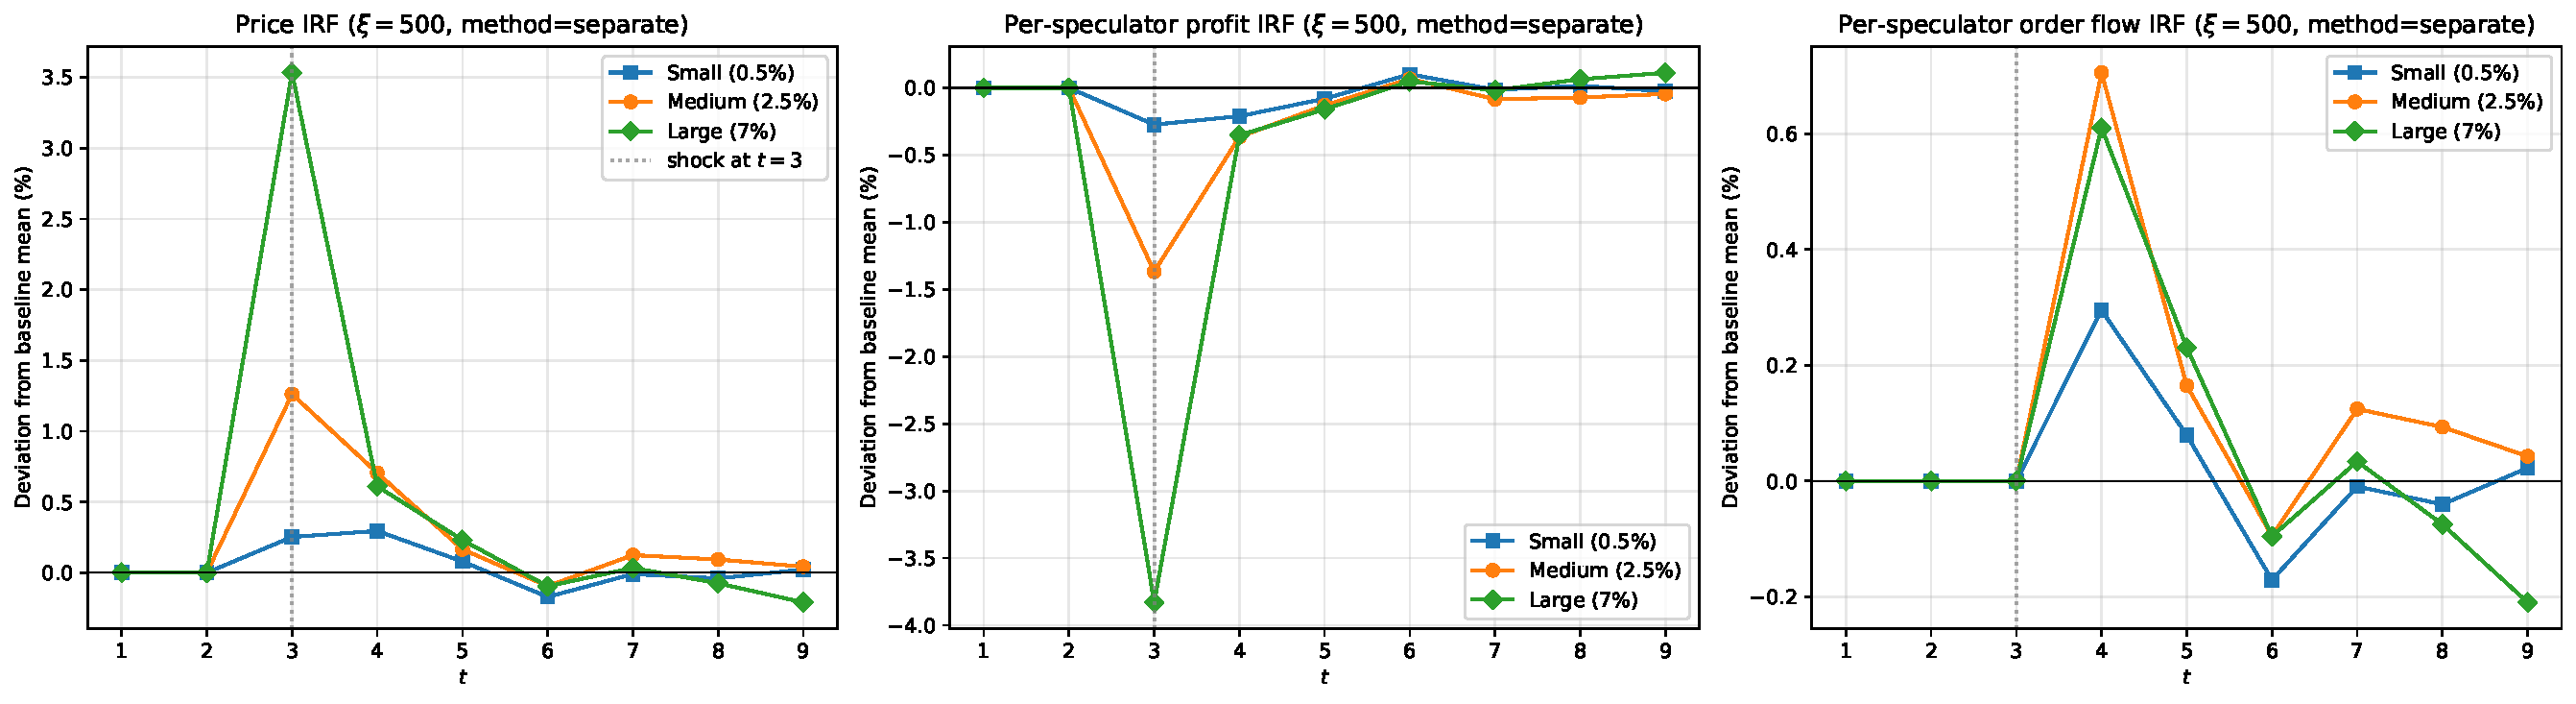
\includegraphics[width=0.85\textwidth]{irf_xi500_separate_I2.pdf}
    \\[0.5em]
    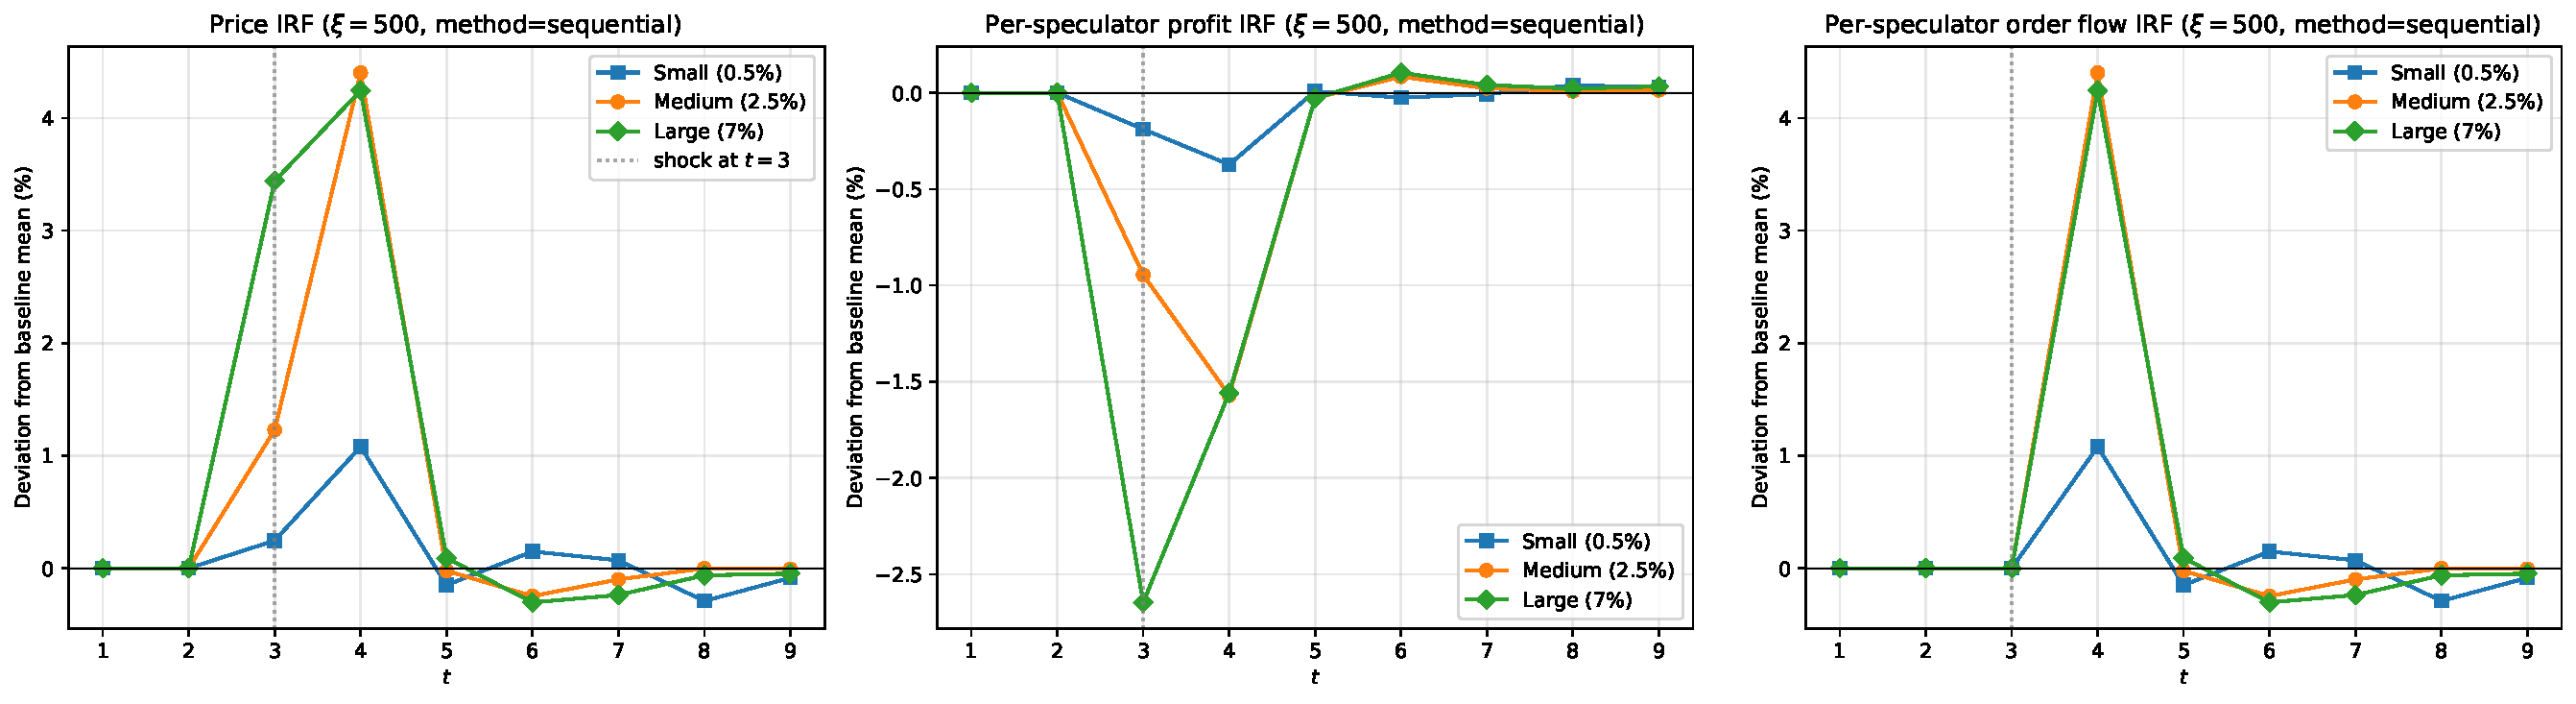
\includegraphics[width=0.85\textwidth]{irf_xi500_sequential_I2.pdf}
    \\[0.5em]
    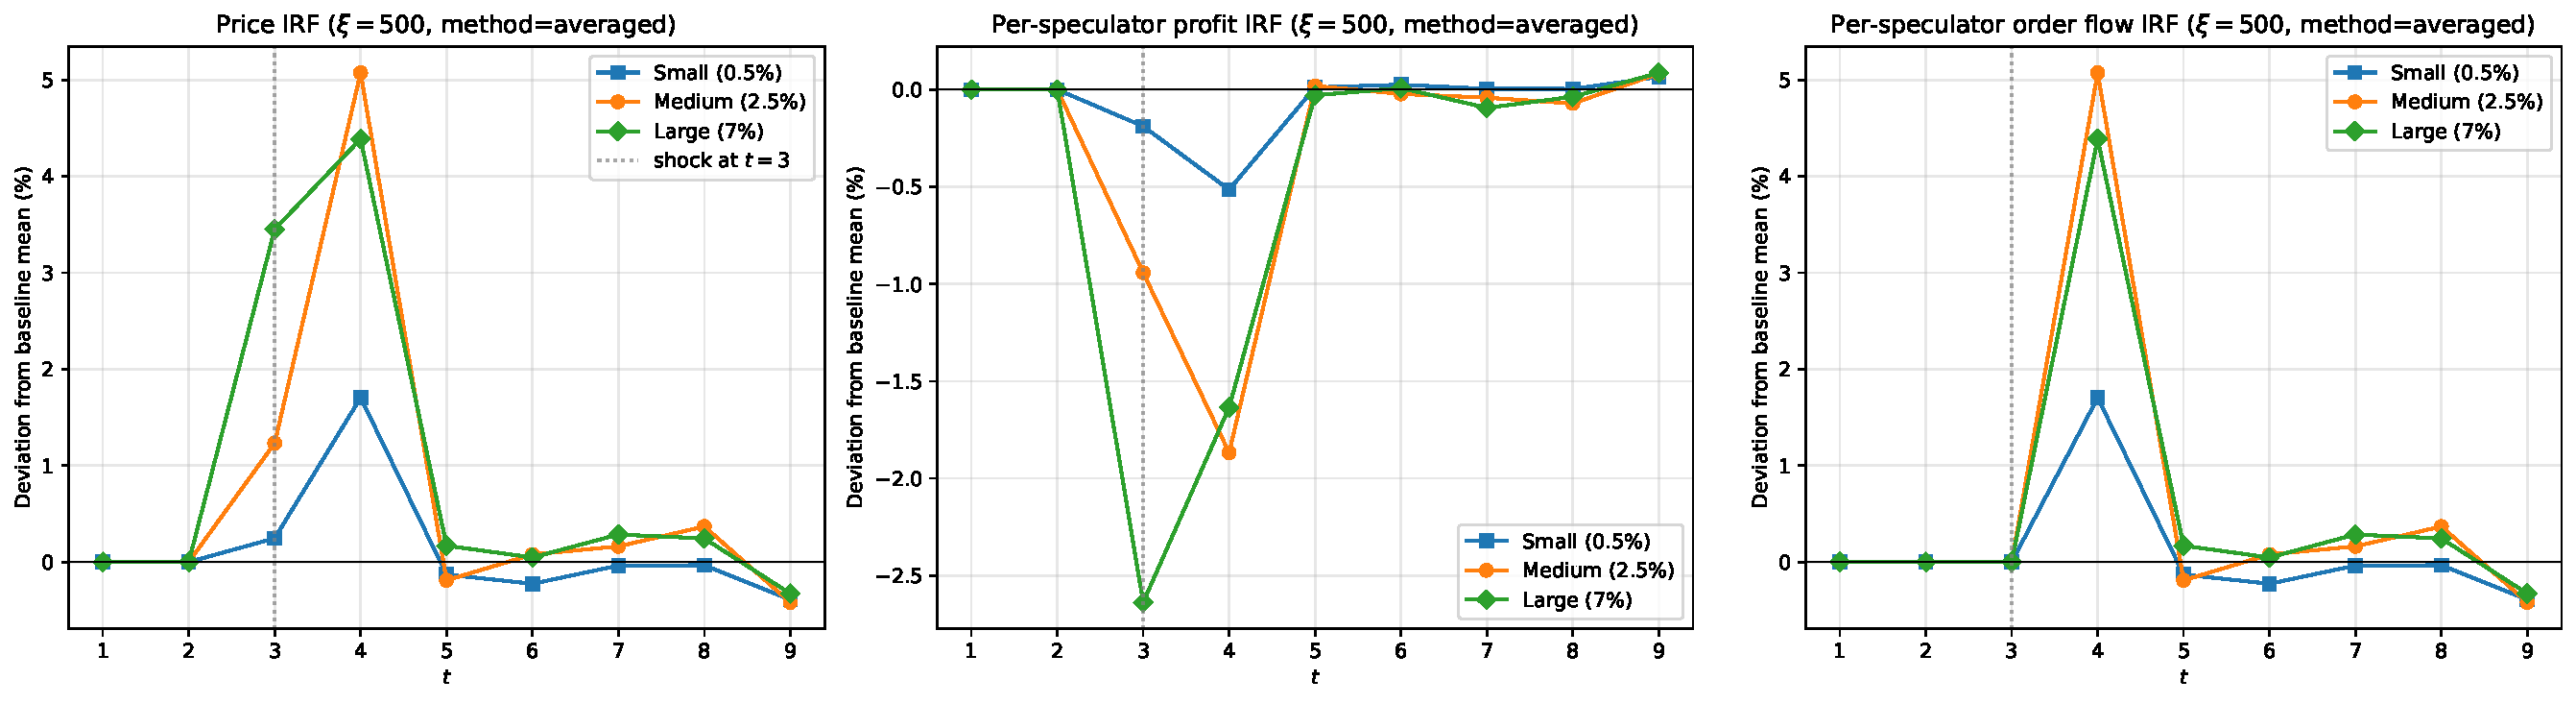
\includegraphics[width=0.85\textwidth]{irf_xi500_averaged_I2.pdf}
    \caption{Impulse response functions at $\xi = 500$ for the three
    update methods (top to bottom: separate, sequential, averaged).
    The shared-Q protocols (middle, bottom) show amplification at $t = 4$ which is consistent with the price-trigger
    mechanism. The separate matrices method (top) shows a weaker but similar pattern.}
    \label{fig:irf_xi500}
\end{figure}

This is the saturation pattern \citet[Figure~3]{Dou2025} identify as the
evidence of a price-trigger punishment scheme: once the trigger
threshold is crossed, both speculators revert to a coordinated
punishment whose intensity is set by the trigger response itself rather
than by the magnitude of the original deviation. An elevated $p_{t-1}$
is read as a sign of defection, and the speculators respond by trading
more aggressively at $t = 4$ to punish the suspected deviator.

The separate-matrices protocol shows a weaker but similar pattern. The small shock generates essentially no response
at $t = 4$ ($\tilde p_4 = -0.05\%$), while the medium and large shocks
produce small but positive amplifications ($\tilde p_4 = 0.21\%$ and
$0.13\%$). The threshold and saturation structure is also preserved, and the
saturation level is much lower than under the shared-Q protocols. This
matches the small-deviation case of \citet{Dou2025}, where shocks below
the threshold fail to trigger a response and the system reverts to
baseline at $t = 4$. The lower saturation level under separate matrices
is consistent with its lower collusion index
($\Delta_\chi^{\text{sep}} = 0.31$ versus
$\Delta_\chi^{\text{shared}} \approx 0.87$): less collusion implies a
less strict punishment.

All three protocols at $\xi=500$ are therefore consistent with price-trigger
collusion. The shared matrix methods deliver a sharper signature than separate matrices,
possibly because common updates accelerate convergence toward conservative actions; the multi-seed evidence in Section~5.2 confirms this gap is a genuine protocol effect rather than session-level noise. The separate-matrices result, which follows the original paper more closely, confirms
that the mechanism is present at $\xi=500$ even at lower intensity.

\section{Conclusion}
The theoretical analysis established the benchmarks: at $\xi=0$, the cartel 
intensity lies below the Nash intensity for $I\ge 2$, per-speculator profits 
satisfy $\pi^M>\pi^N$, and all three market-quality dimensions favor the 
competitive outcome, with the gap widening in $I$, in line with 
\citet{Subrahmanyam1991}. For $\xi>0$, $\lambda$ collapses toward $1/\xi$ and 
quantities rescale by orders of magnitude, but the rankings $\chi^N>\chi^M$ and 
$\pi^M>\pi^N$ are preserved.

The simulations show the collusive outcome emerges in practice across all three 
protocols and both regimes, with $\Delta_\chi$ between roughly $0.3$ and $0.9$. 
The IRF analysis then identifies the mechanism in each regime: at $\xi=0$, no 
$t=4$ adjustment (the over-pruning signature); at $\xi=500$, the threshold and saturation pattern of price-trigger collusion. Despite reaching comparable 
steady-state collusion levels, the two regimes produce qualitatively different 
IRF behavior, validating the two-mechanism theory of the authors within 
our setting. The magnitude is sensitive to the update protocol: separate matrices yields lower $\Delta_\chi$ than a shared Q-matrix, particularly at $\xi=500$; and a 
fuller treatment would estimate session-level distributions across all 
configurations, as \citet{Dou2025} do. However, the main result is clear: algorithms with no shared information, no communication, and no built-in 
incentive to cooperate learn to trade well below the competitive intensity, which suggests that the absence of explicit coordination is not a sufficient safeguard against algorithmic collusion.

% -------------------- REFERENCES --------------------

\begin{thebibliography}{9}

\bibitem[Calvano et al.(2020)]{Calvano2020}
Calvano, E., Calzolari, G., Denicolò, V. and Pastorello, S. (2020).
Artificial intelligence, algorithmic pricing, and collusion.
\textit{American Economic Review}, 110(10), 3267--3297.

\bibitem[Dou et al.(2025)]{Dou2025}
Dou, W. W., Goldstein, I. and Ji, Y. (2025).
AI-powered trading, algorithmic collusion, and price efficiency.
\textit{NBER Working Paper 34054}.

\bibitem[Kyle(1985)]{Kyle1985}
Kyle, A. S. (1985).
Continuous auctions and insider trading.
\textit{Econometrica}, 53(6), 1315--1335.

\bibitem[Subrahmanyam(1991)]{Subrahmanyam1991}
Subrahmanyam, A. (1991).
Risk aversion, market liquidity, and price efficiency.
\textit{Review of Financial Studies}, 4(3), 417--441.

\end{thebibliography}

% -------------------- APPENDIX --------------------
\newpage
\appendix

% ============================================================
% APPENDIX: CODE
% ============================================================
% Required packages (add to preamble if not present):
%   \usepackage{listings}
%   \usepackage{xcolor}
%
% Add this block to the preamble to define the listing styles:
%
% \definecolor{codebg}{rgb}{0.97,0.97,0.97}
% \definecolor{codekw}{rgb}{0.0,0.0,0.6}
% \definecolor{codestr}{rgb}{0.6,0.0,0.0}
% \definecolor{codecmt}{rgb}{0.25,0.5,0.35}
% \lstdefinestyle{pythonstyle}{
%     language=Python,
%     basicstyle=\ttfamily\footnotesize,
%     keywordstyle=\color{codekw}\bfseries,
%     stringstyle=\color{codestr},
%     commentstyle=\color{codecmt}\itshape,
%     backgroundcolor=\color{codebg},
%     numbers=left,
%     numberstyle=\tiny\color{gray},
%     numbersep=6pt,
%     frame=single,
%     framesep=4pt,
%     rulecolor=\color{gray!30},
%     breaklines=true,
%     breakatwhitespace=false,
%     postbreak=\mbox{\textcolor{red}{$\hookrightarrow$}\space},
%     showstringspaces=false,
%     tabsize=4,
%     captionpos=b,
%     upquote=true,
%     literate={—}{{--}}1 {–}{{-}}1 {≈}{{$\\approx$}}1 {≥}{{$\\geq$}}1
%              {≤}{{$\\leq$}}1 {α}{{$\\alpha$}}1 {β}{{$\\beta$}}1
%              {γ}{{$\\gamma$}}1 {θ}{{$\\theta$}}1 {λ}{{$\\lambda$}}1
%              {ξ}{{$\\xi$}}1 {ρ}{{$\\rho$}}1 {σ}{{$\\sigma$}}1
%              {χ}{{$\\chi$}}1 {ε}{{$\\epsilon$}}1 {Δ}{{$\\Delta$}}1
%              {π}{{$\\pi$}}1 {²}{{\\textsuperscript{2}}}1
% }
% \lstdefinestyle{outputstyle}{
%     basicstyle=\ttfamily\footnotesize,
%     backgroundcolor=\color{codebg!50},
%     frame=single,
%     framesep=4pt,
%     rulecolor=\color{gray!20},
%     breaklines=true,
%     breakatwhitespace=false,
%     postbreak=\mbox{\textcolor{red}{$\hookrightarrow$}\space},
%     showstringspaces=false,
%     tabsize=4,
%     upquote=true,
%     literate={—}{{--}}1 {–}{{-}}1 {≈}{{$\\approx$}}1 {≥}{{$\\geq$}}1
%              {≤}{{$\\leq$}}1 {α}{{$\\alpha$}}1 {β}{{$\\beta$}}1
%              {γ}{{$\\gamma$}}1 {θ}{{$\\theta$}}1 {λ}{{$\\lambda$}}1
%              {ξ}{{$\\xi$}}1 {ρ}{{$\\rho$}}1 {σ}{{$\\sigma$}}1
%              {χ}{{$\\chi$}}1 {ε}{{$\\epsilon$}}1 {Δ}{{$\\Delta$}}1
%              {π}{{$\\pi$}}1 {²}{{\\textsuperscript{2}}}1
% }

\section{Code}
\label{sec:code}

This appendix reproduces the Python code used to generate every numerical
and graphical result in the report, together with the textual outputs of
each cell. Plot outputs are omitted here as they appear inline in the main
text. The code is organized by sections and follows the structure of the
accompanying Jupyter notebook.

\subsection{Closed-form Nash and cartel benchmarks}

\begin{lstlisting}[style=pythonstyle]
import numpy as np
import matplotlib.pyplot as plt

# Parameters
sigma_v = 1.0
sigma_u = 0.1
I_values = np.arange(1, 11)

# Closed-form expressions for xi=0
chi_N = sigma_u / (np.sqrt(I_values) * sigma_v)
chi_M = sigma_u / (I_values * sigma_v)
lambda_N = np.sqrt(I_values) * sigma_v / ((I_values + 1) * sigma_u)
lambda_M = sigma_v / (2 * sigma_u) * np.ones_like(I_values, dtype=float)
pi_N = sigma_u * sigma_v / (np.sqrt(I_values) * (I_values + 1))
pi_M = sigma_u * sigma_v / (2 * I_values)
ratio = pi_M / pi_N

# Plotting
fig, axes = plt.subplots(1, 3, figsize=(15, 5))

# Plot 1: lambda^N and lambda^M
axes[0].plot(I_values, lambda_N, 'b-o', label=r'$\lambda^N$')
axes[0].plot(I_values, lambda_M, 'r--s', label=r'$\lambda^M$')
axes[0].set_xlabel(r'Number of speculators $I$')
axes[0].set_ylabel(r'Price impact $\lambda$')
axes[0].set_title(r'Price Impact $\lambda^N$ and $\lambda^M$')
axes[0].legend()
axes[0].grid(True, alpha=0.3)
axes[0].set_xticks(I_values)

# Plot 2: pi^N and pi^M
axes[1].plot(I_values, pi_N, 'b-o', label=r'$\pi^N$')
axes[1].plot(I_values, pi_M, 'r--s', label=r'$\pi^M$')
axes[1].set_xlabel(r'Number of speculators $I$')
axes[1].set_ylabel(r'Per-speculator profit $\pi$')
axes[1].set_title(r'Per-Speculator Profits $\pi^N$ and $\pi^M$')
axes[1].legend()
axes[1].grid(True, alpha=0.3)
axes[1].set_xticks(I_values)

# Plot 3: ratio pi^M/pi^N
axes[2].plot(I_values, ratio, 'g-o', label=r'$\pi^M/\pi^N$')
axes[2].set_xlabel(r'Number of speculators $I$')
axes[2].set_ylabel(r'$\pi^M/\pi^N$')
axes[2].set_title(r'Ratio $\pi^M/\pi^N$')
axes[2].legend()
axes[2].grid(True, alpha=0.3)
axes[2].set_xticks(I_values)

plt.tight_layout()
plt.savefig('lambda_pi_ratio_plots.pdf', bbox_inches='tight')
plt.savefig('lambda_pi_ratio_plots.png', bbox_inches='tight', dpi=150)
plt.close()
print("Plots saved successfully.")

# Print table of values
print(f"\n{'I':>4} {'chi_N':>10} {'chi_M':>10} {'lambda_N':>10} "
      f"{'lambda_M':>10} {'pi_N':>10} {'pi_M':>10} {'pi_M/pi_N':>10}")
print("-" * 80)
for i, I in enumerate(I_values):
    print(f"{I:>4} {chi_N[i]:>10.4f} {chi_M[i]:>10.4f} {lambda_N[i]:>10.4f} "
          f"{lambda_M[i]:>10.4f} {pi_N[i]:>10.4f} {pi_M[i]:>10.4f} {ratio[i]:>10.4f}")
\end{lstlisting}

\noindent\textit{Output:}
\begin{lstlisting}[style=outputstyle]
Plots saved successfully.

   I      chi_N      chi_M   lambda_N   lambda_M       pi_N       pi_M  pi_M/pi_N
--------------------------------------------------------------------------------
   1     0.1000     0.1000     5.0000     5.0000     0.0500     0.0500     1.0000
   2     0.0707     0.0500     4.7140     5.0000     0.0236     0.0250     1.0607
   3     0.0577     0.0333     4.3301     5.0000     0.0144     0.0167     1.1547
   4     0.0500     0.0250     4.0000     5.0000     0.0100     0.0125     1.2500
   5     0.0447     0.0200     3.7268     5.0000     0.0075     0.0100     1.3416
   6     0.0408     0.0167     3.4993     5.0000     0.0058     0.0083     1.4289
   7     0.0378     0.0143     3.3072     5.0000     0.0047     0.0071     1.5119
   8     0.0354     0.0125     3.1427     5.0000     0.0039     0.0063     1.5910
   9     0.0333     0.0111     3.0000     5.0000     0.0033     0.0056     1.6667
  10     0.0316     0.0100     2.8748     5.0000     0.0029     0.0050     1.7393
\end{lstlisting}

\subsection{Market quality at $\xi=0$}

\begin{lstlisting}[style=pythonstyle]
import numpy as np
import matplotlib.pyplot as plt

# Parameters
sigma_v = 1.0
sigma_u = 0.1
I_values = np.arange(1, 11)

# Closed-form expressions (xi = 0)
# Nash equilibrium
chi_N = sigma_u / (np.sqrt(I_values) * sigma_v)
lambda_N = np.sqrt(I_values) * sigma_v / ((I_values + 1) * sigma_u)

# Cartel equilibrium
chi_M = sigma_u / (I_values * sigma_v)
lambda_M = sigma_v / (2 * sigma_u) * np.ones_like(I_values, dtype=float)

# Market quality measures
# Price informativeness: I = (I^2 * chi^2 * sigma_v^2 + sigma_u^2) / (sigma_v^2 * sigma_u^2)
I_N = (I_values**2 * chi_N**2 * sigma_v**2 + sigma_u**2) / (sigma_v**2 * sigma_u**2)
I_M = (I_values**2 * chi_M**2 * sigma_v**2 + sigma_u**2) / (sigma_v**2 * sigma_u**2)

# Noise-trader losses: W_N = lambda * sigma_u^2
W_N_nash = lambda_N * sigma_u**2
W_N_cartel = lambda_M * sigma_u**2

# Plotting
fig, axes = plt.subplots(1, 3, figsize=(15, 5))

# Plot 1: lambda^N and lambda^M
axes[0].plot(I_values, lambda_N, 'b-o', label=r'$\lambda^N$')
axes[0].plot(I_values, lambda_M, 'r--s', label=r'$\lambda^M$')
axes[0].set_xlabel(r'Number of speculators $I$')
axes[0].set_ylabel(r'Price impact $\lambda$')
axes[0].set_title(r'Price Impact $\lambda^N$ and $\lambda^M$')
axes[0].legend()
axes[0].grid(True, alpha=0.3)
axes[0].set_xticks(I_values)

# Plot 2: I^N and I^M
axes[1].plot(I_values, I_N, 'b-o', label=r'$\mathcal{I}^N$')
axes[1].plot(I_values, I_M, 'r--s', label=r'$\mathcal{I}^M$')
axes[1].set_xlabel(r'Number of speculators $I$')
axes[1].set_ylabel(r'Price informativeness $\mathcal{I}$')
axes[1].set_title(r'Price Informativeness $\mathcal{I}^N$ and $\mathcal{I}^M$')
axes[1].legend()
axes[1].grid(True, alpha=0.3)
axes[1].set_xticks(I_values)

# Plot 3: W_N^N and W_N^M
axes[2].plot(I_values, W_N_nash, 'b-o', label=r'$W_N^N$')
axes[2].plot(I_values, W_N_cartel, 'r--s', label=r'$W_N^M$')
axes[2].set_xlabel(r'Number of speculators $I$')
axes[2].set_ylabel(r'Noise-trader losses $W_N$')
axes[2].set_title(r'Noise-Trader Losses $W_N^N$ and $W_N^M$')
axes[2].legend()
axes[2].grid(True, alpha=0.3)
axes[2].set_xticks(I_values)

plt.tight_layout()
plt.savefig('market_quality_plots.pdf', bbox_inches='tight')
plt.close()

print("Plots saved successfully.")

# Print numerical values for verification
print("\nI | lambda_N | lambda_M | I_N    | I_M    | W_N_N  | W_N_M")
print("-" * 70)
for i, I in enumerate(I_values):
    print(f"{I:2d} | {lambda_N[i]:.4f}   | {lambda_M[i]:.4f}   | {I_N[i]:.4f} | {I_M[i]:.4f} | {W_N_nash[i]:.4f} | {W_N_cartel[i]:.4f}")
\end{lstlisting}

\noindent\textit{Output:}
\begin{lstlisting}[style=outputstyle]
Plots saved successfully.

I | lambda_N | lambda_M | I_N    | I_M    | W_N_N  | W_N_M
----------------------------------------------------------------------
 1 | 5.0000   | 5.0000   | 2.0000 | 2.0000 | 0.0500 | 0.0500
 2 | 4.7140   | 5.0000   | 3.0000 | 2.0000 | 0.0471 | 0.0500
 3 | 4.3301   | 5.0000   | 4.0000 | 2.0000 | 0.0433 | 0.0500
 4 | 4.0000   | 5.0000   | 5.0000 | 2.0000 | 0.0400 | 0.0500
 5 | 3.7268   | 5.0000   | 6.0000 | 2.0000 | 0.0373 | 0.0500
 6 | 3.4993   | 5.0000   | 7.0000 | 2.0000 | 0.0350 | 0.0500
 7 | 3.3072   | 5.0000   | 8.0000 | 2.0000 | 0.0331 | 0.0500
 8 | 3.1427   | 5.0000   | 9.0000 | 2.0000 | 0.0314 | 0.0500
 9 | 3.0000   | 5.0000   | 10.0000 | 2.0000 | 0.0300 | 0.0500
10 | 2.8748   | 5.0000   | 11.0000 | 2.0000 | 0.0287 | 0.0500
\end{lstlisting}

\subsection{Numerical equilibrium solver}

\begin{lstlisting}[style=pythonstyle]
import numpy as np
from scipy.optimize import brentq

# Parameters
sigma_v = 1.0
sigma_u = 0.1
theta = 0.1
I = 2
xi_values = [0, 50, 500]

def gamma_func(chi, I, sigma_v, sigma_u):
    """Regression coefficient gamma given chi."""
    return (I * chi) / ((I * chi)**2 + (sigma_u / sigma_v)**2)

def lambda_func(gamma, xi, theta):
    """Price impact lambda given gamma."""
    return (theta * gamma + xi) / (theta + xi**2)

def nash_fixed_point(chi, I, sigma_v, sigma_u, xi, theta):
    """Root gives Nash equilibrium chi^N."""
    g = gamma_func(chi, I, sigma_v, sigma_u)
    lam = lambda_func(g, xi, theta)
    return chi - 1.0 / ((I + 1) * lam)

def cartel_fixed_point(chi, I, sigma_v, sigma_u, xi, theta):
    """Root gives cartel equilibrium chi^M."""
    g = gamma_func(chi, I, sigma_v, sigma_u)
    lam = lambda_func(g, xi, theta)
    return chi - 1.0 / (2 * I * lam)

def find_bracket(f, args, lower=1e-10, start=10.0, factor=10.0, max_iter=20):
    """Automatically expand upper bound until bracket found."""
    upper = start
    for _ in range(max_iter):
        if f(lower, *args) * f(upper, *args) < 0:
            return lower, upper
        upper *= factor
    raise ValueError(f"Could not find bracket after {max_iter} iterations.")

def solve_equilibrium(I, sigma_v, sigma_u, xi, theta):
    """Solve for Nash and cartel equilibria using Brent's method."""
    args = (I, sigma_v, sigma_u, xi, theta)

    # Nash
    a, b = find_bracket(nash_fixed_point, args)
    chi_N = brentq(nash_fixed_point, a, b, args=args)
    gamma_N = gamma_func(chi_N, I, sigma_v, sigma_u)
    lambda_N = lambda_func(gamma_N, xi, theta)
    pi_N = (1 - lambda_N * I * chi_N) * chi_N * sigma_v**2

    # Cartel
    a, b = find_bracket(cartel_fixed_point, args)
    chi_M = brentq(cartel_fixed_point, a, b, args=args)
    gamma_M = gamma_func(chi_M, I, sigma_v, sigma_u)
    lambda_M = lambda_func(gamma_M, xi, theta)
    pi_M = (1 - lambda_M * I * chi_M) * chi_M * sigma_v**2

    return chi_N, lambda_N, pi_N, chi_M, lambda_M, pi_M

# --- Compute and display results ---
print("=" * 80)
print(f"Parameters: I={I}, sigma_v={sigma_v}, sigma_u={sigma_u}, theta={theta}")
print("=" * 80)
print(f"{'xi':>6} | {'chi_N':>10} | {'lambda_N':>10} | {'pi_N':>10} | "
      f"{'chi_M':>10} | {'lambda_M':>10} | {'pi_M':>10}")
print("-" * 80)

results = {}
for xi in xi_values:
    chi_N, lambda_N, pi_N, chi_M, lambda_M, pi_M = solve_equilibrium(
        I, sigma_v, sigma_u, xi, theta)
    results[xi] = (chi_N, lambda_N, pi_N, chi_M, lambda_M, pi_M)
    print(f"{xi:>6} | {chi_N:>10.6f} | {lambda_N:>10.6f} | {pi_N:>10.6f} | "
          f"{chi_M:>10.6f} | {lambda_M:>10.6f} | {pi_M:>10.6f}")

print("=" * 80)

# --- Verify xi=0 against closed forms ---
print("\nVerification against closed forms for xi=0:")
chi_N_cf   = sigma_u / (np.sqrt(I) * sigma_v)
lambda_N_cf = np.sqrt(I) * sigma_v / ((I + 1) * sigma_u)
pi_N_cf    = sigma_u * sigma_v / (np.sqrt(I) * (I + 1))
chi_M_cf   = sigma_u / (I * sigma_v)
lambda_M_cf = sigma_v / (2 * sigma_u)
pi_M_cf    = sigma_u * sigma_v / (2 * I)

print(f"  chi_N:    numerical={results[0][0]:.6f}, closed-form={chi_N_cf:.6f}")
print(f"  lambda_N: numerical={results[0][1]:.6f}, closed-form={lambda_N_cf:.6f}")
print(f"  pi_N:     numerical={results[0][2]:.6f}, closed-form={pi_N_cf:.6f}")
print(f"  chi_M:    numerical={results[0][3]:.6f}, closed-form={chi_M_cf:.6f}")
print(f"  lambda_M: numerical={results[0][4]:.6f}, closed-form={lambda_M_cf:.6f}")
print(f"  pi_M:     numerical={results[0][5]:.6f}, closed-form={pi_M_cf:.6f}")
\end{lstlisting}

\noindent\textit{Output:}
\begin{lstlisting}[style=outputstyle]
================================================================================
Parameters: I=2, sigma_v=1.0, sigma_u=0.1, theta=0.1
================================================================================
    xi |      chi_N |   lambda_N |       pi_N |      chi_M |   lambda_M |       pi_M
--------------------------------------------------------------------------------
     0 |   0.070711 |   4.714045 |   0.023570 |   0.050000 |   5.000000 |   0.025000
    50 |  16.666333 |   0.020000 |   5.555444 |  12.499500 |   0.020001 |   6.249750
   500 | 166.666633 |   0.002000 |  55.555544 | 124.999950 |   0.002000 |  62.499975
================================================================================

Verification against closed forms for xi=0:
  chi_N:    numerical=0.070711, closed-form=0.070711
  lambda_N: numerical=4.714045, closed-form=4.714045
  pi_N:     numerical=0.023570, closed-form=0.023570
  chi_M:    numerical=0.050000, closed-form=0.050000
  lambda_M: numerical=5.000000, closed-form=5.000000
  pi_M:     numerical=0.025000, closed-form=0.025000
\end{lstlisting}

\subsection{Comparative statics at $\xi=500$}

\begin{lstlisting}[style=pythonstyle]
import numpy as np
import matplotlib.pyplot as plt

# Parameters specific to this experiment
xi = 500
I_values = np.arange(1, 11)

# --- Compute for all I ---
chi_N_arr = np.zeros(len(I_values))
lambda_N_arr = np.zeros(len(I_values))
pi_N_arr = np.zeros(len(I_values))
chi_M_arr = np.zeros(len(I_values))
lambda_M_arr = np.zeros(len(I_values))
pi_M_arr = np.zeros(len(I_values))

for idx, I in enumerate(I_values):
    chi_N, lambda_N, pi_N, chi_M, lambda_M, pi_M = solve_equilibrium(
        I, sigma_v, sigma_u, xi, theta
    )
    chi_N_arr[idx] = chi_N
    lambda_N_arr[idx] = lambda_N
    pi_N_arr[idx] = pi_N
    chi_M_arr[idx] = chi_M
    lambda_M_arr[idx] = lambda_M
    pi_M_arr[idx] = pi_M

# --- Market quality measures ---
I_info_N = (I_values**2 * chi_N_arr**2 * sigma_v**2 + sigma_u**2) / (sigma_v**2 * sigma_u**2)
I_info_M = (I_values**2 * chi_M_arr**2 * sigma_v**2 + sigma_u**2) / (sigma_v**2 * sigma_u**2)
W_N_nash   = lambda_N_arr * sigma_u**2
W_N_cartel = lambda_M_arr * sigma_u**2

# --- Print numerical results ---
print(f"xi={xi}, theta={theta}, sigma_v={sigma_v}, sigma_u={sigma_u}")
print(f"{'I':>3} | {'chi_N':>10} | {'lambda_N':>10} | {'pi_N':>10} | {'chi_M':>10} | {'lambda_M':>10} | {'pi_M':>10} | {'I_N':>12} | {'I_M':>12} | {'W_N_N':>10} | {'W_N_M':>10}")
print("-" * 120)
for idx, I in enumerate(I_values):
    print(f"{I:>3} | {chi_N_arr[idx]:>10.4f} | {lambda_N_arr[idx]:>10.6f} | "
          f"{pi_N_arr[idx]:>10.4f} | {chi_M_arr[idx]:>10.4f} | "
          f"{lambda_M_arr[idx]:>10.6f} | {pi_M_arr[idx]:>10.4f} | "
          f"{I_info_N[idx]:>12.4f} | {I_info_M[idx]:>12.4f} | "
          f"{W_N_nash[idx]:>10.6f} | {W_N_cartel[idx]:>10.6f}")

# --- Plots ---
fig, axes = plt.subplots(1, 3, figsize=(15, 5))

axes[0].plot(I_values, lambda_N_arr, 'b-o', label=r'$\lambda^N$')
axes[0].plot(I_values, lambda_M_arr, 'r--s', label=r'$\lambda^M$')
axes[0].set_xlabel(r'Number of speculators $I$')
axes[0].set_ylabel(r'Price impact $\lambda$')
axes[0].set_title(r'Price Impact $\lambda^N$ and $\lambda^M$ ($\xi=500$)')
axes[0].legend()
axes[0].grid(True, alpha=0.3)
axes[0].set_xticks(I_values)

axes[1].plot(I_values, I_info_N, 'b-o', label=r'$\mathcal{I}^N$')
axes[1].plot(I_values, I_info_M, 'r--s', label=r'$\mathcal{I}^M$')
axes[1].set_xlabel(r'Number of speculators $I$')
axes[1].set_ylabel(r'Price informativeness $\mathcal{I}$')
axes[1].set_title(r'Price Informativeness $\mathcal{I}^N$ and $\mathcal{I}^M$ ($\xi=500$)')
axes[1].legend()
axes[1].grid(True, alpha=0.3)
axes[1].set_xticks(I_values)

axes[2].plot(I_values, W_N_nash, 'b-o', label=r'$W_N^N$')
axes[2].plot(I_values, W_N_cartel, 'r--s', label=r'$W_N^M$')
axes[2].set_xlabel(r'Number of speculators $I$')
axes[2].set_ylabel(r'Noise-trader losses $W_N$')
axes[2].set_title(r'Noise-Trader Losses $W_N^N$ and $W_N^M$ ($\xi=500$)')
axes[2].legend()
axes[2].grid(True, alpha=0.3)
axes[2].set_xticks(I_values)

plt.tight_layout()
plt.savefig('comparative_statics_xi500.pdf', bbox_inches='tight')
plt.savefig('comparative_statics_xi500.png', bbox_inches='tight', dpi=150)
plt.close()
print("\nPlots saved.")
\end{lstlisting}

\noindent\textit{Output:}
\begin{lstlisting}[style=outputstyle]
xi=500, theta=0.1, sigma_v=1.0, sigma_u=0.1
  I |      chi_N |   lambda_N |       pi_N |      chi_M |   lambda_M |       pi_M |          I_N |          I_M |      W_N_N |      W_N_M
------------------------------------------------------------------------------------------------------------------------
  1 |   249.9999 |   0.002000 |   125.0000 |   249.9999 |   0.002000 |   125.0000 | 6249996.0000 | 6249996.0000 |   0.000020 |   0.000020
  2 |   166.6666 |   0.002000 |    55.5555 |   125.0000 |   0.002000 |    62.5000 | 11111107.6667 | 6249996.0000 |   0.000020 |   0.000020
  3 |   125.0000 |   0.002000 |    31.2500 |    83.3333 |   0.002000 |    41.6667 | 14062497.2500 | 6249996.0000 |   0.000020 |   0.000020
  4 |   100.0000 |   0.002000 |    20.0000 |    62.5000 |   0.002000 |    31.2500 | 15999997.8000 | 6249996.0000 |   0.000020 |   0.000020
  5 |    83.3333 |   0.002000 |    13.8889 |    50.0000 |   0.002000 |    25.0000 | 17361109.3333 | 6249996.0000 |   0.000020 |   0.000020
  6 |    71.4286 |   0.002000 |    10.2041 |    41.6667 |   0.002000 |    20.8333 | 18367345.4898 | 6249996.0000 |   0.000020 |   0.000020
  7 |    62.5000 |   0.002000 |     7.8125 |    35.7143 |   0.002000 |    17.8571 | 19140623.8125 | 6249996.0000 |   0.000020 |   0.000020
  8 |    55.5556 |   0.002000 |     6.1728 |    31.2500 |   0.002000 |    15.6250 | 19753085.4444 | 6249996.0000 |   0.000020 |   0.000020
  9 |    50.0000 |   0.002000 |     5.0000 |    27.7778 |   0.002000 |    13.8889 | 20249999.2000 | 6249996.0000 |   0.000020 |   0.000020
 10 |    45.4545 |   0.002000 |     4.1322 |    25.0000 |   0.002000 |    12.5000 | 20661156.3719 | 6249996.0000 |   0.000020 |   0.000020

Plots saved.
\end{lstlisting}

\subsection{Effective number of insiders $I^*$}

\begin{lstlisting}[style=pythonstyle]
import numpy as np
from scipy.optimize import brentq

# Parameters
xi_star = 500
theta_star = 0.1
sigma_v_star = 1.0
sigma_u_star = 0.1
I_cases = [2, 3, 5]

def effective_insiders_equation(I_star, lambda_M_target, sigma_v, sigma_u, xi, theta):
    """
    Equation defining I*: lambda^N(I*) - lambda^M(I) = 0.
    Here I* is allowed to be non-integer.
    """
    _, lambda_N, _, _, _, _ = solve_equilibrium(I_star, sigma_v, sigma_u, xi, theta)
    return lambda_N - lambda_M_target

def count_sign_changes(values, tol=1e-10):
    """
    Count sign changes in a sequence, ignoring values very close to zero.
    """
    filtered_signs = []
    for v in values:
        if abs(v) < tol:
            filtered_signs.append(0)
        elif v > 0:
            filtered_signs.append(1)
        else:
            filtered_signs.append(-1)

    changes = 0
    prev = None
    for s in filtered_signs:
        if s == 0:
            continue
        if prev is not None and s != prev:
            changes += 1
        prev = s
    return changes

print("=" * 95)
print(f"Effective number of insiders I* for xi={xi_star}, theta={theta_star}, sigma_v={sigma_v_star}, sigma_u={sigma_u_star}")
print("=" * 95)
print(f"{'I':>5} | {'lambda^M(I)':>12} | {'I*':>12} | {'lambda^N(I*)':>14} | {'Unique on grid?':>16}")
print("-" * 95)

for I in I_cases:
    # Step 1: compute cartel price impact for this I
    _, _, _, _, lambda_M, _ = solve_equilibrium(
        I, sigma_v_star, sigma_u_star, xi_star, theta_star
    )

    # Step 2: define root function f(I*) = lambda^N(I*) - lambda^M(I)
    f = lambda I_star: effective_insiders_equation(
        I_star, lambda_M, sigma_v_star, sigma_u_star, xi_star, theta_star
    )

    # Step 3: bracket a root
    a, b = 1e-6, 1.0
    fa, fb = f(a), f(b)

    while fa * fb > 0:
        b *= 2.0
        fb = f(b)
        if b > 1e6:
            raise ValueError(f"Could not find a bracket for I when I={I}")

    # Step 4: solve for I*
    I_star = brentq(f, a, b, xtol=1e-12)

    # Step 5: verify numerically
    _, lambda_N_check, _, _, _, _ = solve_equilibrium(
        I_star, sigma_v_star, sigma_u_star, xi_star, theta_star
    )

    # Step 6: numerical uniqueness check on a grid
    grid = np.linspace(0.01, 10.0, 2000)
    f_vals = np.array([f(x) for x in grid])
    sign_changes = count_sign_changes(f_vals)
    near_zero_points = np.sum(np.abs(f_vals) < 1e-8)

    # Heuristic uniqueness statement
    unique_flag = "Yes" if sign_changes <= 1 else "Unclear"

    print(f"{I:>5} | {lambda_M:>12.6f} | {I_star:>12.8f} | {lambda_N_check:>14.6f} | {unique_flag:>16}")
\end{lstlisting}

\noindent\textit{Output:}
\begin{lstlisting}[style=outputstyle, basicstyle=\ttfamily\scriptsize]
=========================================================================================
Effective number of insiders I* for xi=500, theta=0.1, sigma_v=1.0, sigma_u=0.1
=========================================================================================
    I |  lambda^M(I) |           I* |   lambda^N(I*) |  Unique on grid?
-----------------------------------------------------------------------------------------
    2 |     0.002000 |   1.00000000 |       0.002000 |              Yes
    3 |     0.002000 |   1.00000000 |       0.002000 |              Yes
    5 |     0.002000 |   1.00000000 |       0.002000 |              Yes
\end{lstlisting}

\subsection{Master function for Q-learning}

\begin{lstlisting}[style=pythonstyle]
import numpy as np
from scipy.stats import norm
from scipy.optimize import brentq
from numba import njit
import time
import matplotlib.pyplot as plt


@njit
def _nearest_idx(value, grid):
    best = 0
    best_diff = abs(grid[0] - value)
    for k in range(1, grid.shape[0]):
        d = abs(grid[k] - value)
        if d < best_diff:
            best_diff = d
            best = k
    return best


@njit
def _train_qlearning(Q, action_grids, price_grids, v_grid,
                     T, alpha, beta, rho, lambda_N, sigma_u, v_bar,
                     I, n_v, n_x, n_p, method_code, seed, report_every):
    """method_code: 0=separate, 1=sequential, 2=averaged."""
    np.random.seed(seed)

    v_prev_idx = np.random.randint(0, n_v)
    v_curr_idx = np.random.randint(0, n_v)
    p_prev_idx = np.random.randint(0, n_p)

    visit_count = np.zeros(n_v, dtype=np.int64)
    n_reports = T // report_every
    chi_history = np.empty(n_reports)
    t_history = np.empty(n_reports, dtype=np.int64)
    report_idx = 0

    action_idx_arr = np.empty(I, dtype=np.int64)
    x_arr = np.empty(I, dtype=np.float64)

    # Per-cell stability tracking (needed for frac_stable_1e6)
    I_eff = I if method_code == 0 else 1
    stored_argmax = np.empty((I_eff, n_p, n_v, n_v), dtype=np.int64)
    last_change_time = np.zeros((I_eff, n_p, n_v, n_v), dtype=np.int64)

    for q_idx in range(I_eff):
        for pp in range(n_p):
            for vv in range(n_v):
                for kk in range(n_v):
                    best_a = 0
                    best_q = Q[q_idx, pp, vv, kk, 0]
                    for a in range(1, n_x):
                        if Q[q_idx, pp, vv, kk, a] > best_q:
                            best_q = Q[q_idx, pp, vv, kk, a]
                            best_a = a
                    stored_argmax[q_idx, pp, vv, kk] = best_a

    frac_stable_1e6 = np.empty(n_reports)

    for t in range(T):
        v_t = v_grid[v_curr_idx]
        epsilon = np.exp(-beta * visit_count[v_curr_idx])

        for i in range(I):
            if np.random.random() < epsilon:
                action_idx_arr[i] = np.random.randint(0, n_x)
            else:
                Q_idx = i if method_code == 0 else 0
                best_a = 0
                best_q = Q[Q_idx, p_prev_idx, v_prev_idx, v_curr_idx, 0]
                for a in range(1, n_x):
                    q_val = Q[Q_idx, p_prev_idx, v_prev_idx, v_curr_idx, a]
                    if q_val > best_q:
                        best_q = q_val
                        best_a = a
                action_idx_arr[i] = best_a
            x_arr[i] = action_grids[v_curr_idx, action_idx_arr[i]]

        u_t = np.random.normal(0.0, sigma_u)
        y_t = 0.0
        for i in range(I):
            y_t += x_arr[i]
        y_t += u_t
        p_t = v_bar + lambda_N * y_t

        v_next_idx = np.random.randint(0, n_v)
        p_t_idx = _nearest_idx(p_t, price_grids[v_curr_idx])

        # Q-update
        if method_code == 0:
            for i in range(I):
                max_q_next = Q[i, p_t_idx, v_curr_idx, v_next_idx, 0]
                for a in range(1, n_x):
                    q_val = Q[i, p_t_idx, v_curr_idx, v_next_idx, a]
                    if q_val > max_q_next:
                        max_q_next = q_val
                pi_it = (v_t - p_t) * x_arr[i]
                target = pi_it + rho * max_q_next
                old = Q[i, p_prev_idx, v_prev_idx, v_curr_idx, action_idx_arr[i]]
                Q[i, p_prev_idx, v_prev_idx, v_curr_idx, action_idx_arr[i]] = \
                    (1.0 - alpha) * old + alpha * target

        elif method_code == 1:
            for i in range(I):
                max_q_next = Q[0, p_t_idx, v_curr_idx, v_next_idx, 0]
                for a in range(1, n_x):
                    q_val = Q[0, p_t_idx, v_curr_idx, v_next_idx, a]
                    if q_val > max_q_next:
                        max_q_next = q_val
                pi_it = (v_t - p_t) * x_arr[i]
                target = pi_it + rho * max_q_next
                old = Q[0, p_prev_idx, v_prev_idx, v_curr_idx, action_idx_arr[i]]
                Q[0, p_prev_idx, v_prev_idx, v_curr_idx, action_idx_arr[i]] = \
                    (1.0 - alpha) * old + alpha * target

        else:  # averaged
            max_q_next = Q[0, p_t_idx, v_curr_idx, v_next_idx, 0]
            for a in range(1, n_x):
                q_val = Q[0, p_t_idx, v_curr_idx, v_next_idx, a]
                if q_val > max_q_next:
                    max_q_next = q_val

            if I == 2:
                a0 = action_idx_arr[0]
                a1 = action_idx_arr[1]
                target_0 = (v_t - p_t) * x_arr[0] + rho * max_q_next
                target_1 = (v_t - p_t) * x_arr[1] + rho * max_q_next
                if a0 == a1:
                    avg_target = 0.5 * (target_0 + target_1)
                    old = Q[0, p_prev_idx, v_prev_idx, v_curr_idx, a0]
                    Q[0, p_prev_idx, v_prev_idx, v_curr_idx, a0] = \
                        (1.0 - alpha) * old + alpha * avg_target
                else:
                    old0 = Q[0, p_prev_idx, v_prev_idx, v_curr_idx, a0]
                    Q[0, p_prev_idx, v_prev_idx, v_curr_idx, a0] = \
                        (1.0 - alpha) * old0 + alpha * target_0
                    old1 = Q[0, p_prev_idx, v_prev_idx, v_curr_idx, a1]
                    Q[0, p_prev_idx, v_prev_idx, v_curr_idx, a1] = \
                        (1.0 - alpha) * old1 + alpha * target_1
            else:
                for i in range(I):
                    pi_it = (v_t - p_t) * x_arr[i]
                    target = pi_it + rho * max_q_next
                    old = Q[0, p_prev_idx, v_prev_idx, v_curr_idx, action_idx_arr[i]]
                    Q[0, p_prev_idx, v_prev_idx, v_curr_idx, action_idx_arr[i]] = \
                        (1.0 - alpha) * old + alpha * target

        # Re-check argmax of just-updated cell, mark flips
        for q_idx in range(I_eff):
            best_a = 0
            best_q = Q[q_idx, p_prev_idx, v_prev_idx, v_curr_idx, 0]
            for a in range(1, n_x):
                q_val = Q[q_idx, p_prev_idx, v_prev_idx, v_curr_idx, a]
                if q_val > best_q:
                    best_q = q_val
                    best_a = a
            if best_a != stored_argmax[q_idx, p_prev_idx, v_prev_idx, v_curr_idx]:
                stored_argmax[q_idx, p_prev_idx, v_prev_idx, v_curr_idx] = best_a
                last_change_time[q_idx, p_prev_idx, v_prev_idx, v_curr_idx] = t + 1

        visit_count[v_curr_idx] += 1
        p_prev_idx = p_t_idx
        v_prev_idx = v_curr_idx
        v_curr_idx = v_next_idx

        # Periodic diagnostic
        if (t + 1) % report_every == 0 and report_idx < n_reports:
            # 1) chi_history (stabilisation of bar chi^C)
            chi_sum = 0.0
            chi_count = 0
            for k in range(n_v):
                dv = v_grid[k] - v_bar
                if abs(dv) > 1e-8:
                    if method_code == 0:
                        mean_a_over_i = 0.0
                        for i in range(I):
                            a_sum = 0.0
                            a_n = 0
                            for pp in range(n_p):
                                for vv in range(n_v):
                                    best_a = 0
                                    best_q = Q[i, pp, vv, k, 0]
                                    for a in range(1, n_x):
                                        q_val = Q[i, pp, vv, k, a]
                                        if q_val > best_q:
                                            best_q = q_val
                                            best_a = a
                                    a_sum += action_grids[k, best_a]
                                    a_n += 1
                            mean_a_over_i += a_sum / a_n
                        mean_a = mean_a_over_i / I
                    else:
                        a_sum = 0.0
                        a_n = 0
                        for pp in range(n_p):
                            for vv in range(n_v):
                                best_a = 0
                                best_q = Q[0, pp, vv, k, 0]
                                for a in range(1, n_x):
                                    q_val = Q[0, pp, vv, k, a]
                                    if q_val > best_q:
                                        best_q = q_val
                                        best_a = a
                                a_sum += action_grids[k, best_a]
                                a_n += 1
                        mean_a = a_sum / a_n
                    chi_sum += mean_a / dv
                    chi_count += 1
            chi_history[report_idx] = chi_sum / chi_count
            t_history[report_idx] = t + 1

            # 2) Fraction of (s,i) cells stable for >= 10^6 consecutive periods
            now = t + 1
            n_total = I_eff * n_p * n_v * n_v
            n_1e6 = 0
            for q_idx in range(I_eff):
                for pp in range(n_p):
                    for vv in range(n_v):
                        for kk in range(n_v):
                            if now - last_change_time[q_idx, pp, vv, kk] >= 1_000_000:
                                n_1e6 += 1
            frac_stable_1e6[report_idx] = n_1e6 / n_total

            report_idx += 1

    return (chi_history[:report_idx],
            t_history[:report_idx],
            visit_count,
            frac_stable_1e6[:report_idx])


@njit
def _evaluate_frozen_policy(Q, action_grids, price_grids, v_grid,
                            T_eval, lambda_N, sigma_u, v_bar,
                            I, n_v, n_x, n_p, method_code, seed):
    np.random.seed(seed)
    v_prev_idx = np.random.randint(0, n_v)
    v_curr_idx = np.random.randint(0, n_v)
    p_prev_idx = np.random.randint(0, n_p)
    v_hist = np.empty(T_eval)
    x_hist = np.empty((T_eval, I))
    for t in range(T_eval):
        v_t = v_grid[v_curr_idx]
        v_hist[t] = v_t
        x_total = 0.0
        for i in range(I):
            Q_idx = i if method_code == 0 else 0
            best_a = 0
            best_q = Q[Q_idx, p_prev_idx, v_prev_idx, v_curr_idx, 0]
            for a in range(1, n_x):
                q_val = Q[Q_idx, p_prev_idx, v_prev_idx, v_curr_idx, a]
                if q_val > best_q:
                    best_q = q_val
                    best_a = a
            x_it = action_grids[v_curr_idx, best_a]
            x_hist[t, i] = x_it
            x_total += x_it
        u_t = np.random.normal(0.0, sigma_u)
        p_t = v_bar + lambda_N * (x_total + u_t)
        v_next_idx = np.random.randint(0, n_v)
        p_t_idx = _nearest_idx(p_t, price_grids[v_curr_idx])
        p_prev_idx = p_t_idx
        v_prev_idx = v_curr_idx
        v_curr_idx = v_next_idx
    return v_hist, x_hist


# =========================================================================
# Equilibrium helpers
# =========================================================================

def _nash_residual(lam, I, sigma_v, sigma_u, theta, xi):
    chi = 1.0 / ((I + 1) * lam)
    gamma = (I * chi) / ((I * chi) ** 2 + (sigma_u / sigma_v) ** 2)
    return lam - (theta * gamma + xi) / (theta + xi ** 2)

def _cartel_residual(lam, I, sigma_v, sigma_u, theta, xi):
    chi = 1.0 / (2 * I * lam)
    gamma = (I * chi) / ((I * chi) ** 2 + (sigma_u / sigma_v) ** 2)
    return lam - (theta * gamma + xi) / (theta + xi ** 2)

def _solve_lambda(residual_fn, I, sigma_v, sigma_u, theta, xi):
    lo, hi = 1e-10, 1.0
    for _ in range(30):
        try:
            if residual_fn(lo, I, sigma_v, sigma_u, theta, xi) * \
               residual_fn(hi, I, sigma_v, sigma_u, theta, xi) < 0:
                break
        except (ZeroDivisionError, OverflowError):
            pass
        hi *= 10
    else:
        raise RuntimeError("Could not bracket lambda.")
    return brentq(residual_fn, lo, hi, args=(I, sigma_v, sigma_u, theta, xi))

def _compute_equilibrium(I, sigma_v, sigma_u, theta, xi):
    if xi == 0:
        chi_N    = sigma_u / (np.sqrt(I) * sigma_v)
        chi_M    = sigma_u / (I * sigma_v)
        lambda_N = np.sqrt(I) * sigma_v / ((I + 1) * sigma_u)
        lambda_M = sigma_v / (2 * sigma_u)
    else:
        lambda_N = _solve_lambda(_nash_residual,   I, sigma_v, sigma_u, theta, xi)
        lambda_M = _solve_lambda(_cartel_residual, I, sigma_v, sigma_u, theta, xi)
        chi_N    = 1.0 / ((I + 1) * lambda_N)
        chi_M    = 1.0 / (2 * I * lambda_M)
    return chi_N, chi_M, lambda_N, lambda_M


# =========================================================================
# Master function
# =========================================================================

def run_qlearning(
    *,
    I=2, xi=0, method="separate",
    T=int(50e6), T_eval=int(1e5),
    v_bar=1.0, sigma_v=1.0, sigma_u=0.1,
    rho=0.95, theta=0.1,
    alpha=0.05, beta=5e-6,
    iota=0.1, n_v=10, n_x=15, n_p=31,
    seed_train=610014, seed_eval=987654,
    save_plot=True, plot_dir=".", verbose=True,
):
    """
    Convergence is reported via two metrics:
      (1) chi_history : trace of bar chi^C over training (stabilisation)
      (2) frac_stable_1e6 : fraction of (s,i) cells whose greedy action has
          remained unchanged for >= 10^6 consecutive periods (softer
          variant of the Dou et al. criterion)

    Returns a dict including:
      'chi_N', 'chi_M', 'lambda_N', 'lambda_M'  - theoretical benchmarks
      'bar_chi_ols', 'Delta_ols'                - primary OLS estimator (IA.4.4)
      'bar_chi_ratio', 'Delta_ratio'            - per-period ratio (diagnostic)
      'chi_per_spec', 'intercept_per_spec'      - per-speculator OLS detail
      'Q', 'Q_list', 'Q_of'                     - Q-matrix + IRF-cell shim
      'chi_history', 't_history'                - bar chi^C trace
      'frac_stable_1e6'                         - fraction stable >= 10^6 per checkpoint
      'v_hist', 'x_hist'                        - frozen-policy sample paths
      'action_grids', 'price_grids', 'v_grid'   - grids
      'train_elapsed'                           - training wall time (s)
    """
    METHOD_CODE = {"separate": 0, "sequential": 1, "averaged": 2}[method]

    if verbose:
        print(f"===== Q-learning: I={I}, xi={xi}, method='{method}', T={T:,} =====")

    chi_N, chi_M, lambda_N, lambda_M = _compute_equilibrium(
        I, sigma_v, sigma_u, theta, xi)
    if verbose:
        print(f"\nBenchmarks (xi={xi}, I={I}):")
        print(f"  chi^N    = {chi_N:.6f}")
        print(f"  chi^M    = {chi_M:.6f}")
        print(f"  lambda^N = {lambda_N:.6e}")
        print(f"  lambda^M = {lambda_M:.6e}")

    # Grids
    k_arr = np.arange(1, n_v + 1)
    v_grid = v_bar + sigma_v * norm.ppf((2 * k_arr - 1) / (2 * n_v))
    x_N_k = chi_N * (v_grid - v_bar)
    x_M_k = chi_M * (v_grid - v_bar)

    action_grids = np.zeros((n_v, n_x))
    for k in range(n_v):
        xN_abs, xM_abs = abs(x_N_k[k]), abs(x_M_k[k])
        width = xN_abs - xM_abs
        pos_lower = xM_abs - iota * width
        pos_upper = xN_abs + iota * width
        if v_grid[k] > v_bar:
            action_grids[k, :] = np.linspace(pos_lower, pos_upper, n_x)
        else:
            action_grids[k, :] = np.linspace(-pos_upper, -pos_lower, n_x)

    price_grids = np.zeros((n_v, n_p))
    for k in range(n_v):
        p_H = v_bar + lambda_N * (I * max(x_M_k[k], x_N_k[k]) + 1.96 * sigma_u)
        p_L = v_bar + lambda_N * (I * min(x_M_k[k], x_N_k[k]) - 1.96 * sigma_u)
        price_grids[k, :] = np.linspace(p_L - iota * (p_H - p_L),
                                        p_H + iota * (p_H - p_L), n_p)

    # Q-init
    Q_init = np.zeros((n_p, n_v, n_v, n_x))
    for k in range(n_v):
        v_k, X_k = v_grid[k], action_grids[k]
        for n in range(n_x):
            x_n = X_k[n]
            total = 0.0
            for m in range(n_x):
                total += (v_k - (v_bar + lambda_N * (x_n + (I - 1) * X_k[m]))) * x_n
            Q_init[:, :, k, n] = total / ((1 - rho) * n_x)

    Q = np.empty((I, n_p, n_v, n_v, n_x))
    for i in range(I):
        Q[i] = Q_init.copy()

    # JIT warm-up
    if verbose:
        print("\nJIT warm-up (T=100)...")
    t0 = time.time()
    Q_warm = Q.copy()
    _train_qlearning(Q_warm, action_grids, price_grids, v_grid,
                     100, alpha, beta, rho, lambda_N, sigma_u, v_bar,
                     I, n_v, n_x, n_p, METHOD_CODE, 0, 50)
    _evaluate_frozen_policy(Q_warm, action_grids, price_grids, v_grid,
                            100, lambda_N, sigma_u, v_bar,
                            I, n_v, n_x, n_p, METHOD_CODE, 1)
    if verbose:
        print(f"Warm-up done in {time.time() - t0:.1f}s")

    # Training
    if verbose:
        print(f"\nTRAINING for T = {T:,} periods...")
    t0 = time.time()
    report_every = max(T // 20, 1)
    (chi_history, t_history, visit_count,
     frac_1e6) = _train_qlearning(
        Q, action_grids, price_grids, v_grid,
        T, alpha, beta, rho, lambda_N, sigma_u, v_bar,
        I, n_v, n_x, n_p, METHOD_CODE, seed_train, report_every
    )
    train_elapsed = time.time() - t0

    if verbose:
        print(f"Training time: {train_elapsed:.1f}s ({train_elapsed/60:.2f} min)")
        print(f"{'t':>14} | {'diag_chi':>9} | {'Delta':>7} | {'frac>=1e6':>10}")
        for j in range(len(t_history)):
            dc = chi_history[j]
            dD = ((chi_N - dc) / (chi_N - chi_M)
                  if abs(chi_N - chi_M) > 1e-12 else np.nan)
            dD_str = "  n/a  " if np.isnan(dD) else f"{dD:7.4f}"
            print(f"  t = {t_history[j]:>10,} | {dc:.6f} | {dD_str} | "
                  f"{100*frac_1e6[j]:9.2f}%")

    # Frozen-policy evaluation
    if verbose:
        print(f"\nEVALUATION for T_eval = {T_eval:,} periods...")
    t0 = time.time()
    v_hist, x_hist = _evaluate_frozen_policy(
        Q, action_grids, price_grids, v_grid,
        T_eval, lambda_N, sigma_u, v_bar,
        I, n_v, n_x, n_p, METHOD_CODE, seed_eval
    )
    if verbose:
        print(f"Evaluation time: {time.time() - t0:.2f}s")

    # Estimators
    chi_per_spec = np.empty(I)
    intercept_per_spec = np.empty(I)
    for i in range(I):
        slope, intercept = np.polyfit(v_hist, x_hist[:, i], 1)
        chi_per_spec[i] = slope
        intercept_per_spec[i] = intercept
    bar_chi_ols = chi_per_spec.mean()

    mask = np.abs(v_hist - v_bar) > 1e-12
    x_bar_t = x_hist.mean(axis=1)
    bar_chi_ratio = (x_bar_t[mask] / (v_hist[mask] - v_bar)).mean()

    if abs(chi_N - chi_M) > 1e-12:
        Delta_ols   = (chi_N - bar_chi_ols)   / (chi_N - chi_M)
        Delta_ratio = (chi_N - bar_chi_ratio) / (chi_N - chi_M)
    else:
        Delta_ols = Delta_ratio = np.nan

    # Report
    if verbose:
        print(f"\n===== Results (I={I}, xi={xi}, method='{method}') =====")
        print(f"  chi^N = {chi_N:.6f}   chi^M = {chi_M:.6f}")
        print(f"  --- Per-speculator OLS (primary, Dou et al. IA.4.4) ---")
        for i in range(I):
            implied = -v_bar * chi_per_spec[i]
            mismatch = 100 * abs(intercept_per_spec[i] - implied) / max(abs(implied), 1e-12)
            print(f"    Spec {i}: chi_hat = {chi_per_spec[i]:.6f} "
                  f"(intercept mismatch = {mismatch:.3f}%)")
        print(f"    bar_chi^C (OLS)      = {bar_chi_ols:.6f}")
        if I >= 2 and abs(bar_chi_ols) > 1e-12:
            asym = 100 * abs(chi_per_spec[0] - chi_per_spec[1]) / abs(bar_chi_ols)
            print(f"    Speculator asymmetry = {asym:.3f}% of mean")
        if not np.isnan(Delta_ols):
            print(f"    Delta_chi (OLS)      = {Delta_ols:.4f}   (0=Nash, 1=cartel)")
        else:
            rel = abs(bar_chi_ols - chi_N) / chi_N * 100
            print(f"    Rel. err vs chi^N    = {rel:.2f}%  (Delta undefined at I=1)")
        print(f"  --- Per-period ratio (diagnostic only) ---")
        print(f"    bar_chi^C (ratio)    = {bar_chi_ratio:.6f}")
        if not np.isnan(Delta_ratio):
            print(f"    Delta_chi (ratio)    = {Delta_ratio:.4f}")

        print(f"  --- Convergence ---")
        print(f"    Cells stable >= 10^6 periods : {100*frac_1e6[-1]:.2f}%")

    # Plot: per-cell stability over training
    if save_plot:
        try:
            fig, ax = plt.subplots(figsize=(10, 6))
            ax.plot(t_history, 100*frac_1e6, 'r-^', markersize=5,
                    label=r'Cells stable for $\geq 10^6$ consecutive periods')
            ax.axhline(100, color='black', linestyle=':', alpha=0.5,
                       label='Full convergence (Dou et al.)')
            ax.set_xlabel('Period $t$')
            ax.set_ylabel('Cells stable (% of total)')
            ax.set_title(rf'Policy stabilisation ($I={I}$, $\xi={xi}$, method="{method}")')
            ax.set_ylim(0, 105)
            ax.legend(loc='lower right')
            ax.grid(True, alpha=0.3)
            plt.tight_layout()
            fname = (f'{plot_dir}/convergence_I{I}_xi{xi}_{method}'
                     f'_a{alpha}_b{beta:.0e}')
            plt.savefig(f'{fname}.pdf', bbox_inches='tight')
            plt.savefig(f'{fname}.png', bbox_inches='tight', dpi=150)
            plt.close()
            if verbose:
                print(f"\nPlot saved: {fname}.pdf / .png")
        except Exception as e:
            if verbose:
                print(f"\nPlotting skipped: {e}")

    # Compatibility shim
    if method == "separate":
        Q_list = [Q[i] for i in range(I)]
    else:
        Q_list = [Q[0]]

    def Q_of(agent_idx):
        return Q_list[agent_idx] if method == "separate" else Q_list[0]

    return {
        'I': I,
        'xi': xi,
        'method': method,
        'T': T,
        'T_eval': T_eval,
        'v_bar': v_bar,
        'sigma_v': sigma_v,
        'sigma_u': sigma_u,
        'rho': rho,
        'theta': theta,
        'alpha': alpha,
        'beta': beta,
        'iota': iota,
        'n_v': n_v,
        'n_x': n_x,
        'n_p': n_p,
        'seed_train': seed_train,
        'seed_eval': seed_eval,

        'chi_N': chi_N, 'chi_M': chi_M,
        'lambda_N': lambda_N, 'lambda_M': lambda_M,
        'bar_chi_ols': bar_chi_ols, 'Delta_ols': Delta_ols,
        'bar_chi_ratio': bar_chi_ratio, 'Delta_ratio': Delta_ratio,
        'chi_per_spec': chi_per_spec, 'intercept_per_spec': intercept_per_spec,
        'Q': Q, 'Q_list': Q_list, 'Q_of': Q_of,
        'chi_history': chi_history, 't_history': t_history,
        'frac_stable_1e6': frac_1e6,
        'v_hist': v_hist, 'x_hist': x_hist,
        'action_grids': action_grids, 'price_grids': price_grids, 'v_grid': v_grid,
        'train_elapsed': train_elapsed,
    }
\end{lstlisting}

\subsection{$I=1$ sanity check}

\begin{lstlisting}[style=pythonstyle]
res_sanity = run_qlearning(I=1, xi=0, method="separate", T=int(10e6))
\end{lstlisting}

\noindent\textit{Output:}
\begin{lstlisting}[style=outputstyle]
===== Q-learning: I=1, xi=0, method='separate', T=10,000,000 =====

Benchmarks (xi=0, I=1):
  chi^N    = 0.100000
  chi^M    = 0.100000
  lambda^N = 5.000000e+00
  lambda^M = 5.000000e+00

JIT warm-up (T=100)...
Warm-up done in 1.6s

TRAINING for T = 10,000,000 periods...
Training time: 1.5s (0.02 min)
             t |  diag_chi |   Delta |  frac>=1e6
  t =    500,000 | 0.100000 |   n/a   |      0.00%
  t =  1,000,000 | 0.100000 |   n/a   |      0.13%
  t =  1,500,000 | 0.100000 |   n/a   |     65.65%
  t =  2,000,000 | 0.100000 |   n/a   |     69.48%
  t =  2,500,000 | 0.100000 |   n/a   |     60.16%
  t =  3,000,000 | 0.100000 |   n/a   |     50.10%
  t =  3,500,000 | 0.100000 |   n/a   |     44.68%
  t =  4,000,000 | 0.100000 |   n/a   |     40.45%
  t =  4,500,000 | 0.100000 |   n/a   |     37.42%
  t =  5,000,000 | 0.100000 |   n/a   |     35.13%
  t =  5,500,000 | 0.100000 |   n/a   |     32.32%
  t =  6,000,000 | 0.100000 |   n/a   |     30.45%
  t =  6,500,000 | 0.100000 |   n/a   |     28.74%
  t =  7,000,000 | 0.100000 |   n/a   |     27.16%
  t =  7,500,000 | 0.100000 |   n/a   |     25.61%
  t =  8,000,000 | 0.100000 |   n/a   |     24.87%
  t =  8,500,000 | 0.100000 |   n/a   |     23.81%
  t =  9,000,000 | 0.100000 |   n/a   |     23.19%
  t =  9,500,000 | 0.100000 |   n/a   |     22.52%
  t = 10,000,000 | 0.100000 |   n/a   |     21.87%

EVALUATION for T_eval = 100,000 periods...
Evaluation time: 0.01s

===== Results (I=1, xi=0, method='separate') =====
  chi^N = 0.100000   chi^M = 0.100000
  --- Per-speculator OLS (primary, Dou et al. IA.4.4) ---
    Spec 0: chi_hat = 0.100000 (intercept mismatch = 0.000%)
    bar_chi^C (OLS)      = 0.100000
    Rel. err vs chi^N    = 0.00%  (Delta undefined at I=1)
  --- Per-period ratio (diagnostic only) ---
    bar_chi^C (ratio)    = 0.100000
  --- Convergence ---
    Cells stable >= 10^6 periods : 21.87%

Plot saved: ./convergence_I1_xi0_separate_a0.05_b5e-06.pdf / .png
\end{lstlisting}

\subsection{$I=2$, $\xi=0$ method comparison}

\begin{lstlisting}[style=pythonstyle]
# --- xi=0, I=2 baseline + method comparison ---
results_by_method = {}
for m in ("separate", "sequential", "averaged"):
    results_by_method[m] = run_qlearning(
        I=2, xi=0, method=m, T=int(500e6), verbose=True
    )
res_xi0 = results_by_method["separate"]

# --- Summary ---
print(f"\nNash:   chi^N = {res_xi0['chi_N']:.4f}")
print(f"Cartel: chi^M = {res_xi0['chi_M']:.4f}\n")
for m, res in results_by_method.items():
    print(f"  {m:<12}  bar_chi^C = {res['bar_chi_ols']:.4f}  "
          f"Delta = {res['Delta_ols']:.4f}")
\end{lstlisting}

\noindent\textit{Output:}
\begin{lstlisting}[style=outputstyle]
===== Q-learning: I=2, xi=0, method='separate', T=500,000,000 =====

Benchmarks (xi=0, I=2):
  chi^N    = 0.070711
  chi^M    = 0.050000
  lambda^N = 4.714045e+00
  lambda^M = 5.000000e+00

JIT warm-up (T=100)...
Warm-up done in 0.0s

TRAINING for T = 500,000,000 periods...
Training time: 83.8s (1.40 min)
             t |  diag_chi |   Delta |  frac>=1e6
  t = 25,000,000 | 0.060833 |  0.4769 |     15.73%
  t = 50,000,000 | 0.060556 |  0.4903 |     19.19%
  t = 75,000,000 | 0.059996 |  0.5174 |     53.31%
  t = 100,000,000 | 0.059449 |  0.5438 |     72.29%
  t = 125,000,000 | 0.058986 |  0.5661 |     88.68%
  t = 150,000,000 | 0.058842 |  0.5731 |     92.65%
  t = 175,000,000 | 0.058616 |  0.5840 |     90.61%
  t = 200,000,000 | 0.058381 |  0.5954 |     97.47%
  t = 225,000,000 | 0.058285 |  0.6000 |     97.10%
  t = 250,000,000 | 0.058194 |  0.6043 |     97.47%
  t = 275,000,000 | 0.057965 |  0.6154 |     97.74%
  t = 300,000,000 | 0.058022 |  0.6127 |     98.03%
  t = 325,000,000 | 0.057902 |  0.6185 |     98.65%
  t = 350,000,000 | 0.057852 |  0.6209 |     98.94%
  t = 375,000,000 | 0.057770 |  0.6248 |     98.95%
  t = 400,000,000 | 0.057820 |  0.6224 |     98.53%
  t = 425,000,000 | 0.057845 |  0.6212 |     99.10%
  t = 450,000,000 | 0.057844 |  0.6213 |     98.52%
  t = 475,000,000 | 0.057818 |  0.6225 |     97.76%
  t = 500,000,000 | 0.057777 |  0.6245 |     98.52%

EVALUATION for T_eval = 100,000 periods...
Evaluation time: 0.01s

===== Results (I=2, xi=0, method='separate') =====
  chi^N = 0.070711   chi^M = 0.050000
  --- Per-speculator OLS (primary, Dou et al. IA.4.4) ---
    Spec 0: chi_hat = 0.055840 (intercept mismatch = 0.137%)
    Spec 1: chi_hat = 0.055778 (intercept mismatch = 0.003%)
    bar_chi^C (OLS)      = 0.055809
    Speculator asymmetry = 0.111% of mean
    Delta_chi (OLS)      = 0.7195   (0=Nash, 1=cartel)
  --- Per-period ratio (diagnostic only) ---
    bar_chi^C (ratio)    = 0.057161
    Delta_chi (ratio)    = 0.6543
  --- Convergence ---
    Cells stable >= 10^6 periods : 98.52%

Plot saved: ./convergence_I2_xi0_separate_a0.05_b5e-06.pdf / .png
===== Q-learning: I=2, xi=0, method='sequential', T=500,000,000 =====

Benchmarks (xi=0, I=2):
  chi^N    = 0.070711
  chi^M    = 0.050000
  lambda^N = 4.714045e+00
  lambda^M = 5.000000e+00

JIT warm-up (T=100)...
Warm-up done in 0.0s

TRAINING for T = 500,000,000 periods...
Training time: 70.6s (1.18 min)
             t |  diag_chi |   Delta |  frac>=1e6
  t = 25,000,000 | 0.058493 |  0.5899 |      6.42%
  t = 50,000,000 | 0.057218 |  0.6515 |     45.26%
  t = 75,000,000 | 0.056277 |  0.6969 |     83.68%
  t = 100,000,000 | 0.055916 |  0.7143 |     83.90%
  t = 125,000,000 | 0.055676 |  0.7260 |     89.19%
  t = 150,000,000 | 0.055400 |  0.7393 |     92.52%
  t = 175,000,000 | 0.055441 |  0.7373 |     91.29%
  t = 200,000,000 | 0.055137 |  0.7520 |     96.39%
  t = 225,000,000 | 0.055003 |  0.7584 |     95.81%
  t = 250,000,000 | 0.055141 |  0.7518 |     96.10%
  t = 275,000,000 | 0.054928 |  0.7621 |     95.58%
  t = 300,000,000 | 0.054860 |  0.7654 |     95.97%
  t = 325,000,000 | 0.054771 |  0.7696 |     97.48%
  t = 350,000,000 | 0.054708 |  0.7727 |     97.55%
  t = 375,000,000 | 0.054706 |  0.7728 |     98.74%
  t = 400,000,000 | 0.054660 |  0.7750 |     98.16%
  t = 425,000,000 | 0.054699 |  0.7731 |     97.32%
  t = 450,000,000 | 0.054582 |  0.7787 |     98.19%
  t = 475,000,000 | 0.054599 |  0.7780 |     96.06%
  t = 500,000,000 | 0.054520 |  0.7818 |     98.10%

EVALUATION for T_eval = 100,000 periods...
Evaluation time: 0.01s

===== Results (I=2, xi=0, method='sequential') =====
  chi^N = 0.070711   chi^M = 0.050000
  --- Per-speculator OLS (primary, Dou et al. IA.4.4) ---
    Spec 0: chi_hat = 0.051687 (intercept mismatch = 0.177%)
    Spec 1: chi_hat = 0.051687 (intercept mismatch = 0.177%)
    bar_chi^C (OLS)      = 0.051687
    Speculator asymmetry = 0.000% of mean
    Delta_chi (OLS)      = 0.9186   (0=Nash, 1=cartel)
  --- Per-period ratio (diagnostic only) ---
    bar_chi^C (ratio)    = 0.054005
    Delta_chi (ratio)    = 0.8066
  --- Convergence ---
    Cells stable >= 10^6 periods : 98.10%

Plot saved: ./convergence_I2_xi0_sequential_a0.05_b5e-06.pdf / .png
===== Q-learning: I=2, xi=0, method='averaged', T=500,000,000 =====

Benchmarks (xi=0, I=2):
  chi^N    = 0.070711
  chi^M    = 0.050000
  lambda^N = 4.714045e+00
  lambda^M = 5.000000e+00

JIT warm-up (T=100)...
Warm-up done in 0.0s

TRAINING for T = 500,000,000 periods...
Training time: 69.8s (1.16 min)
             t |  diag_chi |   Delta |  frac>=1e6
  t = 25,000,000 | 0.059246 |  0.5536 |      8.00%
  t = 50,000,000 | 0.058424 |  0.5933 |     11.42%
  t = 75,000,000 | 0.057471 |  0.6393 |     46.42%
  t = 100,000,000 | 0.056958 |  0.6640 |     67.16%
  t = 125,000,000 | 0.056366 |  0.6926 |     82.48%
  t = 150,000,000 | 0.056055 |  0.7076 |     89.03%
  t = 175,000,000 | 0.055899 |  0.7152 |     86.48%
  t = 200,000,000 | 0.055820 |  0.7190 |     92.87%
  t = 225,000,000 | 0.055538 |  0.7326 |     95.23%
  t = 250,000,000 | 0.055507 |  0.7341 |     95.10%
  t = 275,000,000 | 0.055244 |  0.7468 |     95.29%
  t = 300,000,000 | 0.055480 |  0.7354 |     95.61%
  t = 325,000,000 | 0.055317 |  0.7433 |     97.74%
  t = 350,000,000 | 0.055293 |  0.7444 |     97.42%
  t = 375,000,000 | 0.055362 |  0.7411 |     97.35%
  t = 400,000,000 | 0.055218 |  0.7481 |     97.23%
  t = 425,000,000 | 0.055079 |  0.7548 |     98.23%
  t = 450,000,000 | 0.054963 |  0.7604 |     97.87%
  t = 475,000,000 | 0.055114 |  0.7531 |     96.55%
  t = 500,000,000 | 0.054998 |  0.7587 |     98.35%

EVALUATION for T_eval = 100,000 periods...
Evaluation time: 0.01s

===== Results (I=2, xi=0, method='averaged') =====
  chi^N = 0.070711   chi^M = 0.050000
  --- Per-speculator OLS (primary, Dou et al. IA.4.4) ---
    Spec 0: chi_hat = 0.052032 (intercept mismatch = 0.016%)
    Spec 1: chi_hat = 0.052032 (intercept mismatch = 0.016%)
    bar_chi^C (OLS)      = 0.052032
    Speculator asymmetry = 0.000% of mean
    Delta_chi (OLS)      = 0.9019   (0=Nash, 1=cartel)
  --- Per-period ratio (diagnostic only) ---
    bar_chi^C (ratio)    = 0.054560
    Delta_chi (ratio)    = 0.7798
  --- Convergence ---
    Cells stable >= 10^6 periods : 98.35%

Plot saved: ./convergence_I2_xi0_averaged_a0.05_b5e-06.pdf / .png

Nash:   chi^N = 0.0707
Cartel: chi^M = 0.0500

  separate      bar_chi^C = 0.0558  Delta = 0.7195
  sequential    bar_chi^C = 0.0517  Delta = 0.9186
  averaged      bar_chi^C = 0.0520  Delta = 0.9019
\end{lstlisting}

\subsection{$I=2$, $\xi=500$ method comparison}

\begin{lstlisting}[style=pythonstyle]
# --- xi=500, I=2 baseline + method comparison ---
results_xi500 = {}
for m in ("separate", "sequential", "averaged"):
    results_xi500[m] = run_qlearning(
        I=2, xi=500, method=m, T=int(500e6), verbose=True
    )
res_xi500 = results_xi500["separate"]

# --- Summary ---
print(f"\nNash:   chi^N = {res_xi500['chi_N']:.4f}")
print(f"Cartel: chi^M = {res_xi500['chi_M']:.4f}\n")
for m, res in results_xi500.items():
    print(f"  {m:<12}  bar_chi^C = {res['bar_chi_ols']:.4f}  "
          f"Delta = {res['Delta_ols']:.4f}")
\end{lstlisting}

\noindent\textit{Output:}
\begin{lstlisting}[style=outputstyle]
===== Q-learning: I=2, xi=500, method='separate', T=500,000,000 =====

Benchmarks (xi=500, I=2):
  chi^N    = 166.666633
  chi^M    = 124.999950
  lambda^N = 2.000000e-03
  lambda^M = 2.000001e-03

JIT warm-up (T=100)...
Warm-up done in 0.0s

TRAINING for T = 500,000,000 periods...
Training time: 80.2s (1.34 min)
             t |  diag_chi |   Delta |  frac>=1e6
  t = 25,000,000 | 146.632255 |  0.4808 |      8.11%
  t = 50,000,000 | 147.718661 |  0.4548 |      9.63%
  t = 75,000,000 | 147.923154 |  0.4498 |     30.18%
  t = 100,000,000 | 148.891473 |  0.4266 |     42.60%
  t = 125,000,000 | 149.464630 |  0.4128 |     61.61%
  t = 150,000,000 | 150.575229 |  0.3862 |     71.23%
  t = 175,000,000 | 150.469238 |  0.3887 |     80.31%
  t = 200,000,000 | 150.529722 |  0.3873 |     86.39%
  t = 225,000,000 | 150.790667 |  0.3810 |     85.53%
  t = 250,000,000 | 151.318893 |  0.3683 |     94.21%
  t = 275,000,000 | 151.444469 |  0.3653 |     93.19%
  t = 300,000,000 | 150.973271 |  0.3766 |     95.26%
  t = 325,000,000 | 150.687556 |  0.3835 |     97.16%
  t = 350,000,000 | 150.941589 |  0.3774 |     95.05%
  t = 375,000,000 | 151.093086 |  0.3738 |     97.65%
  t = 400,000,000 | 150.910483 |  0.3781 |     96.71%
  t = 425,000,000 | 150.966358 |  0.3768 |     97.08%
  t = 450,000,000 | 151.427188 |  0.3657 |     96.02%
  t = 475,000,000 | 151.208294 |  0.3710 |     91.34%
  t = 500,000,000 | 151.408179 |  0.3662 |     96.50%

EVALUATION for T_eval = 100,000 periods...
Evaluation time: 0.01s

===== Results (I=2, xi=500, method='separate') =====
  chi^N = 166.666633   chi^M = 124.999950
  --- Per-speculator OLS (primary, Dou et al. IA.4.4) ---
    Spec 0: chi_hat = 154.109664 (intercept mismatch = 0.357%)
    Spec 1: chi_hat = 153.497437 (intercept mismatch = 0.343%)
    bar_chi^C (OLS)      = 153.803550
    Speculator asymmetry = 0.398% of mean
    Delta_chi (OLS)      = 0.3087   (0=Nash, 1=cartel)
  --- Per-period ratio (diagnostic only) ---
    bar_chi^C (ratio)    = 150.939312
    Delta_chi (ratio)    = 0.3775
  --- Convergence ---
    Cells stable >= 10^6 periods : 96.50%

Plot saved: ./convergence_I2_xi500_separate_a0.05_b5e-06.pdf / .png
===== Q-learning: I=2, xi=500, method='sequential', T=500,000,000 =====

Benchmarks (xi=500, I=2):
  chi^N    = 166.666633
  chi^M    = 124.999950
  lambda^N = 2.000000e-03
  lambda^M = 2.000001e-03

JIT warm-up (T=100)...
Warm-up done in 0.0s

TRAINING for T = 500,000,000 periods...
Training time: 69.4s (1.16 min)
             t |  diag_chi |   Delta |  frac>=1e6
  t = 25,000,000 | 144.213475 |  0.5389 |     31.48%
  t = 50,000,000 | 142.465779 |  0.5808 |     57.81%
  t = 75,000,000 | 141.340202 |  0.6078 |     89.03%
  t = 100,000,000 | 141.973843 |  0.5926 |     74.74%
  t = 125,000,000 | 141.507253 |  0.6038 |     93.03%
  t = 150,000,000 | 141.754949 |  0.5979 |     92.26%
  t = 175,000,000 | 141.396654 |  0.6065 |     95.39%
  t = 200,000,000 | 141.037207 |  0.6151 |     97.23%
  t = 225,000,000 | 141.261861 |  0.6097 |     95.19%
  t = 250,000,000 | 141.181216 |  0.6116 |     96.58%
  t = 275,000,000 | 141.018774 |  0.6155 |     96.81%
  t = 300,000,000 | 141.227299 |  0.6105 |     95.77%
  t = 325,000,000 | 141.295271 |  0.6089 |     97.29%
  t = 350,000,000 | 140.973843 |  0.6166 |     97.39%
  t = 375,000,000 | 141.072921 |  0.6142 |     97.45%
  t = 400,000,000 | 141.026838 |  0.6154 |     96.00%
  t = 425,000,000 | 140.506101 |  0.6279 |     97.97%
  t = 450,000,000 | 140.303336 |  0.6327 |     98.77%
  t = 475,000,000 | 140.280294 |  0.6333 |     98.26%
  t = 500,000,000 | 140.612091 |  0.6253 |     98.13%

EVALUATION for T_eval = 100,000 periods...
Evaluation time: 0.01s

===== Results (I=2, xi=500, method='sequential') =====
  chi^N = 166.666633   chi^M = 124.999950
  --- Per-speculator OLS (primary, Dou et al. IA.4.4) ---
    Spec 0: chi_hat = 130.600242 (intercept mismatch = 0.162%)
    Spec 1: chi_hat = 130.600242 (intercept mismatch = 0.162%)
    bar_chi^C (OLS)      = 130.600242
    Speculator asymmetry = 0.000% of mean
    Delta_chi (OLS)      = 0.8656   (0=Nash, 1=cartel)
  --- Per-period ratio (diagnostic only) ---
    bar_chi^C (ratio)    = 137.226217
    Delta_chi (ratio)    = 0.7066
  --- Convergence ---
    Cells stable >= 10^6 periods : 98.13%

Plot saved: ./convergence_I2_xi500_sequential_a0.05_b5e-06.pdf / .png
===== Q-learning: I=2, xi=500, method='averaged', T=500,000,000 =====

Benchmarks (xi=500, I=2):
  chi^N    = 166.666633
  chi^M    = 124.999950
  lambda^N = 2.000000e-03
  lambda^M = 2.000001e-03

JIT warm-up (T=100)...
Warm-up done in 0.0s

TRAINING for T = 500,000,000 periods...
Training time: 65.5s (1.09 min)
             t |  diag_chi |   Delta |  frac>=1e6
  t = 25,000,000 | 144.833291 |  0.5240 |     30.94%
  t = 50,000,000 | 143.792968 |  0.5490 |     36.03%
  t = 75,000,000 | 142.322922 |  0.5842 |     73.65%
  t = 100,000,000 | 142.415088 |  0.5820 |     74.06%
  t = 125,000,000 | 141.337898 |  0.6079 |     91.48%
  t = 150,000,000 | 141.670848 |  0.5999 |     86.55%
  t = 175,000,000 | 141.394350 |  0.6065 |     92.55%
  t = 200,000,000 | 141.023382 |  0.6154 |     93.65%
  t = 225,000,000 | 141.339050 |  0.6079 |     89.68%
  t = 250,000,000 | 141.248036 |  0.6100 |     94.81%
  t = 275,000,000 | 141.061400 |  0.6145 |     96.23%
  t = 300,000,000 | 140.880525 |  0.6189 |     95.61%
  t = 325,000,000 | 140.775686 |  0.6214 |     96.71%
  t = 350,000,000 | 141.127069 |  0.6129 |     95.58%
  t = 375,000,000 | 141.125917 |  0.6130 |     97.61%
  t = 400,000,000 | 141.051032 |  0.6148 |     97.65%
  t = 425,000,000 | 140.661631 |  0.6241 |     98.13%
  t = 450,000,000 | 140.580985 |  0.6261 |     97.29%
  t = 475,000,000 | 140.734211 |  0.6224 |     97.06%
  t = 500,000,000 | 140.530294 |  0.6273 |     97.52%

EVALUATION for T_eval = 100,000 periods...
Evaluation time: 0.01s

===== Results (I=2, xi=500, method='averaged') =====
  chi^N = 166.666633   chi^M = 124.999950
  --- Per-speculator OLS (primary, Dou et al. IA.4.4) ---
    Spec 0: chi_hat = 130.645157 (intercept mismatch = 0.210%)
    Spec 1: chi_hat = 130.645157 (intercept mismatch = 0.210%)
    bar_chi^C (OLS)      = 130.645157
    Speculator asymmetry = 0.000% of mean
    Delta_chi (OLS)      = 0.8645   (0=Nash, 1=cartel)
  --- Per-period ratio (diagnostic only) ---
    bar_chi^C (ratio)    = 136.995538
    Delta_chi (ratio)    = 0.7121
  --- Convergence ---
    Cells stable >= 10^6 periods : 97.52%

Plot saved: ./convergence_I2_xi500_averaged_a0.05_b5e-06.pdf / .png

Nash:   chi^N = 166.6666
Cartel: chi^M = 125.0000

  separate      bar_chi^C = 153.8036  Delta = 0.3087
  sequential    bar_chi^C = 130.6002  Delta = 0.8656
  averaged      bar_chi^C = 130.6452  Delta = 0.8645
\end{lstlisting}

\subsection{Master function for IRF analysis}

\begin{lstlisting}[style=pythonstyle]
def run_irf_analysis(
    qres,
    *,
    Nsim=1000,
    H=9,
    shock_period=2,          # 0-indexed, so 2 means t=3
    shock_sizes_pct=(0.005, 0.025, 0.07),
    shock_labels=("Small (0.5%)", "Medium (2.5%)", "Large (7%)"),
    seed_cal=123,
    seed_irf=20260610,
    T_cal=20_000,
    save_plot=True,
    plot_dir=".",
    use_per_speculator_order_flow=True,
    verbose=True,
):
    """
    Noise-shock impulse response analysis.

    Input
    -----
    qres : dict
        Output of run_qlearning(...)

    Returns
    -------
    dict with:
        results
        E_abs_x
        shock_sizes
        t_axis
        filename_base
    """

    import numpy as np
    import matplotlib.pyplot as plt
    import time

    start = time.time()

    Q_list = qres["Q_list"]
    action_grids = qres["action_grids"]
    price_grids = qres["price_grids"]
    v_grid = qres["v_grid"]

    v_bar = qres.get("v_bar", 1.0) if "v_bar" in qres else 1.0
    sigma_u = qres.get("sigma_u", 0.1) if "sigma_u" in qres else 0.1
    lambda_N = qres["lambda_N"]

    I = qres.get("I", None)
    method = qres.get("method", None)
    xi = qres.get("xi", None)

    # Fallbacks if not stored in qres
    if I is None:
        I = len(Q_list) if len(Q_list) > 1 else 2
    if method is None:
        method = "separate" if len(Q_list) == I else "shared"
    if xi is None:
        xi = "unknown"

    n_v = len(v_grid)
    n_p = price_grids.shape[1]

    if verbose:
        print(f"=== IRF analysis for xi={xi}, I={I}, method='{method}' ===\n")

    def nearest_idx(value, grid):
        return int(np.argmin(np.abs(grid - value)))

    def Q_of(i):
        return Q_list[i] if method == "separate" else Q_list[0]

    # ============================================================
    # Step 1: compute E[|x_i|] under frozen greedy policy
    # ============================================================
    if verbose:
        print("Computing E[|x_i|] under frozen greedy policy...")

    rng_cal = np.random.default_rng(seed_cal)

    v_prev_idx = rng_cal.integers(0, n_v)
    v_curr_idx = rng_cal.integers(0, n_v)
    p_prev_idx = rng_cal.integers(0, n_p)

    abs_x_samples = []

    for _ in range(T_cal):
        x_total = 0.0
        x_arr = np.empty(I)

        for i in range(I):
            ai = np.argmax(Q_of(i)[p_prev_idx, v_prev_idx, v_curr_idx, :])
            xi_i = action_grids[v_curr_idx, ai]
            x_arr[i] = xi_i
            x_total += xi_i

        abs_x_samples.extend(np.abs(x_arr))

        u_t = rng_cal.normal(0, sigma_u)
        p_t = v_bar + lambda_N * (x_total + u_t)

        v_next_idx = rng_cal.integers(0, n_v)
        p_t_idx = nearest_idx(p_t, price_grids[v_curr_idx])

        p_prev_idx = p_t_idx
        v_prev_idx = v_curr_idx
        v_curr_idx = v_next_idx

    E_abs_x = float(np.mean(abs_x_samples))
    shock_sizes = [pct * E_abs_x for pct in shock_sizes_pct]

    if verbose:
        print(f"  E[|x_i|] = {E_abs_x:.6f}")
        for pct, size in zip(shock_sizes_pct, shock_sizes):
            print(f"  Shock size {100*pct:.1f}% => u_shock = {size:.6f}")
        print()

    # ============================================================
    # Step 2: pre-draw common random numbers
    # ============================================================
    rng_irf = np.random.default_rng(seed_irf)

    v0_idx_arr = rng_irf.integers(0, n_v, size=Nsim)
    p0_idx_arr = rng_irf.integers(0, n_p, size=Nsim)
    v_seq_idx_arr = rng_irf.integers(0, n_v, size=(Nsim, H))
    u_seq_arr = rng_irf.normal(0, sigma_u, size=(Nsim, H))
    v_seq_arr = v_grid[v_seq_idx_arr]

    # ============================================================
    # Step 3: frozen-policy simulator
    # ============================================================
    def simulate_path(v_seq_idx, v_seq, u_seq, v0_idx, p0_idx, shock_size=0.0):
        p_rec = np.empty(H)
        x_rec = np.empty(H)
        pi_avg_rec = np.empty(H)

        p_prev_idx = p0_idx
        v_prev_idx = v0_idx

        for t in range(H):
            v_curr_idx = v_seq_idx[t]
            v_t = v_seq[t]

            x_total = 0.0
            x_arr = np.empty(I)

            for i in range(I):
                ai = np.argmax(Q_of(i)[p_prev_idx, v_prev_idx, v_curr_idx, :])
                xi_i = action_grids[v_curr_idx, ai]
                x_arr[i] = xi_i
                x_total += xi_i

            u_t = u_seq[t]
            if t == shock_period and shock_size != 0.0:
                u_t += shock_size * np.sign(v_t - v_bar)

            p_t = v_bar + lambda_N * (x_total + u_t)

            pi_avg = np.mean((v_t - p_t) * x_arr)

            p_rec[t] = p_t

            if use_per_speculator_order_flow:
                x_rec[t] = np.mean(x_arr)
            else:
                x_rec[t] = x_total

            pi_avg_rec[t] = pi_avg

            p_t_idx = nearest_idx(p_t, price_grids[v_curr_idx])
            p_prev_idx = p_t_idx
            v_prev_idx = v_curr_idx

        return p_rec, x_rec, pi_avg_rec

    # ============================================================
    # Step 4: run baseline vs shocked simulations
    # ============================================================
    results = {}

    for s_label, s_size in zip(shock_labels, shock_sizes):
        if verbose:
            print(f"Running IRF for shock = {s_label} ...")

        t0 = time.time()

        p_base = np.empty((Nsim, H))
        x_base = np.empty((Nsim, H))
        pi_base = np.empty((Nsim, H))

        p_shk = np.empty((Nsim, H))
        x_shk = np.empty((Nsim, H))
        pi_shk = np.empty((Nsim, H))

        for n in range(Nsim):
            pb, xb, pib = simulate_path(
                v_seq_idx_arr[n], v_seq_arr[n], u_seq_arr[n],
                v0_idx_arr[n], p0_idx_arr[n],
                shock_size=0.0,
            )

            ps, xs, pis = simulate_path(
                v_seq_idx_arr[n], v_seq_arr[n], u_seq_arr[n],
                v0_idx_arr[n], p0_idx_arr[n],
                shock_size=s_size,
            )

            p_base[n] = pb
            x_base[n] = xb
            pi_base[n] = pib

            p_shk[n] = ps
            x_shk[n] = xs
            pi_shk[n] = pis

        sgn = np.sign(v_seq_arr - v_bar)

        p_tilde_b = (p_base - v_bar) * sgn
        p_tilde_s = (p_shk - v_bar) * sgn

        x_tilde_b = x_base * sgn
        x_tilde_s = x_shk * sgn

        p_b_mean = p_tilde_b.mean(axis=0)
        p_s_mean = p_tilde_s.mean(axis=0)

        x_b_mean = x_tilde_b.mean(axis=0)
        x_s_mean = x_tilde_s.mean(axis=0)

        pi_b_mean = pi_base.mean(axis=0)
        pi_s_mean = pi_shk.mean(axis=0)

        eps = 1e-12
        p_pct = 100.0 * (p_s_mean - p_b_mean) / np.where(np.abs(p_b_mean) < eps, np.nan, p_b_mean)
        x_pct = 100.0 * (x_s_mean - x_b_mean) / np.where(np.abs(x_b_mean) < eps, np.nan, x_b_mean)
        pi_pct = 100.0 * (pi_s_mean - pi_b_mean) / np.where(np.abs(pi_b_mean) < eps, np.nan, pi_b_mean)

        results[s_label] = {
            "p_pct": p_pct,
            "x_pct": x_pct,
            "pi_pct": pi_pct,
            "p_b_mean": p_b_mean,
            "x_b_mean": x_b_mean,
            "pi_b_mean": pi_b_mean,
            "p_s_mean": p_s_mean,
            "x_s_mean": x_s_mean,
            "pi_s_mean": pi_s_mean,
        }

        if verbose:
            print(f"  Done in {time.time() - t0:.1f}s")

    # ============================================================
    # Step 5: plot
    # ============================================================
    t_axis = np.arange(1, H + 1)
    filename_base = f"{plot_dir}/irf_xi{xi}_{method}_I{I}"

    if save_plot:
        if verbose:
            print("\nGenerating IRF plots...")

        fig, axes = plt.subplots(1, 3, figsize=(18, 5))
        markers = ["s", "o", "D"]

        for (label, r), m in zip(results.items(), markers):
            axes[0].plot(t_axis, r["p_pct"], marker=m, label=label, markersize=6)
        axes[0].axvline(shock_period + 1, color="gray", linestyle=":", alpha=0.7, label="shock at $t=3$")
        axes[0].axhline(0.0, color="black", linewidth=0.5)
        axes[0].set_xlabel("$t$")
        axes[0].set_ylabel("Deviation from baseline mean (%)")
        axes[0].set_title(rf"Price IRF ($\xi={xi}$, method={method})")
        axes[0].legend()
        axes[0].grid(True, alpha=0.3)

        for (label, r), m in zip(results.items(), markers):
            axes[1].plot(t_axis, r["pi_pct"], marker=m, label=label, markersize=6)
        axes[1].axvline(shock_period + 1, color="gray", linestyle=":", alpha=0.7)
        axes[1].axhline(0.0, color="black", linewidth=0.5)
        axes[1].set_xlabel("$t$")
        axes[1].set_ylabel("Deviation from baseline mean (%)")
        axes[1].set_title(rf"Per-speculator profit IRF ($\xi={xi}$, method={method})")
        axes[1].legend()
        axes[1].grid(True, alpha=0.3)

        x_title = "Per-speculator order flow" if use_per_speculator_order_flow else "Total informed order flow"

        for (label, r), m in zip(results.items(), markers):
            axes[2].plot(t_axis, r["x_pct"], marker=m, label=label, markersize=6)
        axes[2].axvline(shock_period + 1, color="gray", linestyle=":", alpha=0.7)
        axes[2].axhline(0.0, color="black", linewidth=0.5)
        axes[2].set_xlabel("$t$")
        axes[2].set_ylabel("Deviation from baseline mean (%)")
        axes[2].set_title(rf"{x_title} IRF ($\xi={xi}$, method={method})")
        axes[2].legend()
        axes[2].grid(True, alpha=0.3)

        plt.tight_layout()
        plt.savefig(f"{filename_base}.pdf", bbox_inches="tight")
        plt.savefig(f"{filename_base}.png", bbox_inches="tight", dpi=150)
        plt.close()

        if verbose:
            print(f"IRF plot saved as {filename_base}.pdf / .png")

    # ============================================================
    # Step 6: numerical summary
    # ============================================================
    if verbose:
        print(f"\n===== IRF numerical summary for xi={xi}, method={method}, I={I} =====")

        for label, r in results.items():
            print(f"\nShock = {label}")
            print("  t  |  price (%)  |  profit (%) |  order flow (%)")
            print("  ---|-------------|-------------|----------------")
            for t in range(H):
                print(
                    f"  {t+1:>2} | {r['p_pct'][t]:>10.3f}  | "
                    f"{r['pi_pct'][t]:>10.3f}  | {r['x_pct'][t]:>10.3f}"
                )

        print(f"\nTotal IRF runtime: {time.time() - start:.1f}s")

    return {
        "results": results,
        "E_abs_x": E_abs_x,
        "shock_sizes": shock_sizes,
        "shock_sizes_pct": shock_sizes_pct,
        "shock_labels": shock_labels,
        "t_axis": t_axis,
        "filename_base": filename_base,
        "use_per_speculator_order_flow": use_per_speculator_order_flow,
    }
\end{lstlisting}

\subsection{IRF analysis at $\xi=0$}

\begin{lstlisting}[style=pythonstyle]
# --- IRF analysis: xi=0, I=2, all methods ---
irf_xi0 = {}

for m, res in results_by_method.items():
    print(f"\n===== IRF: xi=0, method='{m}' =====")

    irf_xi0[m] = run_irf_analysis(
        res,
        verbose=True,
        save_plot=True,
        plot_dir="."
    )
\end{lstlisting}

\noindent\textit{Output:}
\begin{lstlisting}[style=outputstyle]

===== IRF: xi=0, method='separate' =====
=== IRF analysis for xi=0, I=2, method='separate' ===

Computing E[|x_i|] under frozen greedy policy...
  E[|x_i|] = 0.043639
  Shock size 0.5% => u_shock = 0.000218
  Shock size 2.5% => u_shock = 0.001091
  Shock size 7.0% => u_shock = 0.003055

Running IRF for shock = Small (0.5%) ...
  Done in 0.2s
Running IRF for shock = Medium (2.5%) ...
  Done in 0.2s
Running IRF for shock = Large (7%) ...
  Done in 0.2s

Generating IRF plots...
IRF plot saved as ./irf_xi0_separate_I2.pdf / .png

===== IRF numerical summary for xi=0, method=separate, I=2 =====

Shock = Small (0.5%)
  t  |  price (%)  |  profit (%) |  order flow (%)
  ---|-------------|-------------|----------------
   1 |      0.000  |      0.000  |      0.000
   2 |      0.000  |      0.000  |      0.000
   3 |      0.261  |     -0.180  |      0.000
   4 |      0.015  |      0.001  |      0.015
   5 |      0.000  |      0.000  |      0.000
   6 |      0.000  |      0.000  |      0.000
   7 |      0.000  |      0.000  |      0.000
   8 |      0.000  |      0.000  |      0.000
   9 |      0.000  |      0.000  |      0.000

Shock = Medium (2.5%)
  t  |  price (%)  |  profit (%) |  order flow (%)
  ---|-------------|-------------|----------------
   1 |      0.000  |      0.000  |      0.000
   2 |      0.000  |      0.000  |      0.000
   3 |      1.307  |     -0.898  |      0.000
   4 |     -0.027  |     -0.152  |     -0.027
   5 |     -0.058  |     -0.026  |     -0.062
   6 |      0.070  |     -0.005  |      0.069
   7 |     -0.017  |     -0.000  |     -0.017
   8 |     -0.008  |      0.007  |     -0.008
   9 |      0.000  |      0.000  |      0.000

Shock = Large (7%)
  t  |  price (%)  |  profit (%) |  order flow (%)
  ---|-------------|-------------|----------------
   1 |      0.000  |      0.000  |      0.000
   2 |      0.000  |      0.000  |      0.000
   3 |      3.660  |     -2.516  |      0.000
   4 |     -0.212  |     -0.088  |     -0.212
   5 |     -0.073  |     -0.099  |     -0.077
   6 |      0.093  |     -0.129  |      0.091
   7 |      0.007  |     -0.012  |      0.007
   8 |     -0.026  |      0.010  |     -0.027
   9 |     -0.001  |     -0.001  |     -0.001

Total IRF runtime: 1.4s

===== IRF: xi=0, method='sequential' =====
=== IRF analysis for xi=0, I=2, method='sequential' ===

Computing E[|x_i|] under frozen greedy policy...
  E[|x_i|] = 0.040686
  Shock size 0.5% => u_shock = 0.000203
  Shock size 2.5% => u_shock = 0.001017
  Shock size 7.0% => u_shock = 0.002848

Running IRF for shock = Small (0.5%) ...
  Done in 0.2s
Running IRF for shock = Medium (2.5%) ...
  Done in 0.2s
Running IRF for shock = Large (7%) ...
  Done in 0.2s

Generating IRF plots...
IRF plot saved as ./irf_xi0_sequential_I2.pdf / .png

===== IRF numerical summary for xi=0, method=sequential, I=2 =====

Shock = Small (0.5%)
  t  |  price (%)  |  profit (%) |  order flow (%)
  ---|-------------|-------------|----------------
   1 |      0.000  |      0.000  |      0.000
   2 |      0.000  |      0.000  |      0.000
   3 |      0.265  |     -0.154  |      0.000
   4 |     -0.022  |     -0.005  |     -0.022
   5 |      0.043  |      0.002  |      0.045
   6 |      0.002  |     -0.001  |      0.002
   7 |      0.000  |      0.000  |      0.000
   8 |      0.000  |      0.000  |      0.000
   9 |      0.000  |      0.000  |      0.000

Shock = Medium (2.5%)
  t  |  price (%)  |  profit (%) |  order flow (%)
  ---|-------------|-------------|----------------
   1 |      0.000  |      0.000  |      0.000
   2 |      0.000  |      0.000  |      0.000
   3 |      1.325  |     -0.770  |      0.000
   4 |     -0.060  |     -0.061  |     -0.060
   5 |      0.105  |     -0.052  |      0.111
   6 |     -0.010  |     -0.000  |     -0.010
   7 |      0.000  |      0.000  |      0.000
   8 |      0.000  |      0.000  |      0.000
   9 |      0.000  |      0.000  |      0.000

Shock = Large (7%)
  t  |  price (%)  |  profit (%) |  order flow (%)
  ---|-------------|-------------|----------------
   1 |      0.000  |      0.000  |      0.000
   2 |      0.000  |      0.000  |      0.000
   3 |      3.711  |     -2.156  |      0.000
   4 |      0.204  |     -0.125  |      0.204
   5 |      0.335  |     -0.122  |      0.355
   6 |      0.018  |      0.020  |      0.017
   7 |     -0.001  |     -0.005  |     -0.001
   8 |      0.000  |      0.000  |      0.000
   9 |      0.000  |      0.000  |      0.000

Total IRF runtime: 1.5s

===== IRF: xi=0, method='averaged' =====
=== IRF analysis for xi=0, I=2, method='averaged' ===

Computing E[|x_i|] under frozen greedy policy...
  E[|x_i|] = 0.041000
  Shock size 0.5% => u_shock = 0.000205
  Shock size 2.5% => u_shock = 0.001025
  Shock size 7.0% => u_shock = 0.002870

Running IRF for shock = Small (0.5%) ...
  Done in 0.2s
Running IRF for shock = Medium (2.5%) ...
  Done in 0.2s
Running IRF for shock = Large (7%) ...
  Done in 0.2s

Generating IRF plots...
IRF plot saved as ./irf_xi0_averaged_I2.pdf / .png

===== IRF numerical summary for xi=0, method=averaged, I=2 =====

Shock = Small (0.5%)
  t  |  price (%)  |  profit (%) |  order flow (%)
  ---|-------------|-------------|----------------
   1 |      0.000  |      0.000  |      0.000
   2 |      0.000  |      0.000  |      0.000
   3 |      0.262  |     -0.158  |      0.000
   4 |      0.014  |      0.019  |      0.014
   5 |      0.019  |     -0.030  |      0.020
   6 |     -0.009  |      0.004  |     -0.009
   7 |      0.000  |      0.000  |      0.000
   8 |      0.000  |      0.000  |      0.000
   9 |      0.000  |      0.000  |      0.000

Shock = Medium (2.5%)
  t  |  price (%)  |  profit (%) |  order flow (%)
  ---|-------------|-------------|----------------
   1 |      0.000  |      0.000  |      0.000
   2 |      0.000  |      0.000  |      0.000
   3 |      1.310  |     -0.792  |      0.000
   4 |     -0.031  |     -0.211  |     -0.031
   5 |      0.049  |     -0.058  |      0.052
   6 |      0.008  |     -0.012  |      0.007
   7 |     -0.036  |      0.009  |     -0.035
   8 |     -0.009  |     -0.005  |     -0.009
   9 |      0.006  |     -0.001  |      0.006

Shock = Large (7%)
  t  |  price (%)  |  profit (%) |  order flow (%)
  ---|-------------|-------------|----------------
   1 |      0.000  |      0.000  |      0.000
   2 |      0.000  |      0.000  |      0.000
   3 |      3.668  |     -2.218  |      0.000
   4 |     -0.327  |     -0.240  |     -0.327
   5 |      0.068  |      0.053  |      0.073
   6 |     -0.047  |     -0.074  |     -0.045
   7 |     -0.018  |     -0.037  |     -0.018
   8 |     -0.030  |      0.007  |     -0.031
   9 |      0.008  |      0.000  |      0.007

Total IRF runtime: 1.4s
\end{lstlisting}

\subsection{IRF analysis at $\xi=500$}

\begin{lstlisting}[style=pythonstyle]
# --- IRF analysis: xi=500, I=2, all methods ---
irf_xi500 = {}

for m, res in results_xi500.items():
    print(f"\n===== IRF: xi=500, method='{m}' =====")

    irf_xi500[m] = run_irf_analysis(
        res,
        verbose=True,
        save_plot=True,
        plot_dir="."
    )
\end{lstlisting}

\noindent\textit{Output:}
\begin{lstlisting}[style=outputstyle]

===== IRF: xi=500, method='separate' =====
=== IRF analysis for xi=500, I=2, method='separate' ===

Computing E[|x_i|] under frozen greedy policy...
  E[|x_i|] = 119.020678
  Shock size 0.5% => u_shock = 0.595103
  Shock size 2.5% => u_shock = 2.975517
  Shock size 7.0% => u_shock = 8.331447

Running IRF for shock = Small (0.5%) ...
  Done in 0.2s
Running IRF for shock = Medium (2.5%) ...
  Done in 0.2s
Running IRF for shock = Large (7%) ...
  Done in 0.2s

Generating IRF plots...
IRF plot saved as ./irf_xi500_separate_I2.pdf / .png

===== IRF numerical summary for xi=500, method=separate, I=2 =====

Shock = Small (0.5%)
  t  |  price (%)  |  profit (%) |  order flow (%)
  ---|-------------|-------------|----------------
   1 |      0.000  |      0.000  |      0.000
   2 |      0.000  |      0.000  |      0.000
   3 |      0.246  |     -0.266  |      0.000
   4 |     -0.048  |      0.004  |     -0.048
   5 |      0.484  |     -0.290  |      0.484
   6 |     -0.076  |     -0.008  |     -0.076
   7 |     -0.028  |      0.013  |     -0.028
   8 |     -0.058  |     -0.007  |     -0.058
   9 |     -0.057  |      0.037  |     -0.057

Shock = Medium (2.5%)
  t  |  price (%)  |  profit (%) |  order flow (%)
  ---|-------------|-------------|----------------
   1 |      0.000  |      0.000  |      0.000
   2 |      0.000  |      0.000  |      0.000
   3 |      1.228  |     -1.331  |      0.000
   4 |      0.212  |     -0.080  |      0.212
   5 |      0.606  |     -0.455  |      0.606
   6 |      0.468  |     -0.415  |      0.468
   7 |      0.115  |     -0.049  |      0.115
   8 |      0.063  |     -0.078  |      0.063
   9 |      0.411  |     -0.270  |      0.411

Shock = Large (7%)
  t  |  price (%)  |  profit (%) |  order flow (%)
  ---|-------------|-------------|----------------
   1 |      0.000  |      0.000  |      0.000
   2 |      0.000  |      0.000  |      0.000
   3 |      3.439  |     -3.726  |      0.000
   4 |      0.132  |     -0.039  |      0.132
   5 |      0.589  |     -0.460  |      0.589
   6 |      0.258  |     -0.139  |      0.258
   7 |     -0.032  |      0.001  |     -0.032
   8 |     -0.289  |      0.064  |     -0.289
   9 |      0.222  |     -0.126  |      0.222

Total IRF runtime: 1.5s

===== IRF: xi=500, method='sequential' =====
=== IRF analysis for xi=500, I=2, method='sequential' ===

Computing E[|x_i|] under frozen greedy policy...
  E[|x_i|] = 103.190489
  Shock size 0.5% => u_shock = 0.515952
  Shock size 2.5% => u_shock = 2.579762
  Shock size 7.0% => u_shock = 7.223334

Running IRF for shock = Small (0.5%) ...
  Done in 0.2s
Running IRF for shock = Medium (2.5%) ...
  Done in 0.2s
Running IRF for shock = Large (7%) ...
  Done in 0.2s

Generating IRF plots...
IRF plot saved as ./irf_xi500_sequential_I2.pdf / .png

===== IRF numerical summary for xi=500, method=sequential, I=2 =====

Shock = Small (0.5%)
  t  |  price (%)  |  profit (%) |  order flow (%)
  ---|-------------|-------------|----------------
   1 |      0.000  |      0.000  |      0.000
   2 |      0.000  |      0.000  |      0.000
   3 |      0.246  |     -0.189  |      0.000
   4 |      1.079  |     -0.372  |      1.079
   5 |     -0.150  |      0.008  |     -0.150
   6 |      0.148  |     -0.025  |      0.148
   7 |      0.070  |     -0.007  |      0.070
   8 |     -0.291  |      0.040  |     -0.291
   9 |     -0.086  |      0.028  |     -0.086

Shock = Medium (2.5%)
  t  |  price (%)  |  profit (%) |  order flow (%)
  ---|-------------|-------------|----------------
   1 |      0.000  |      0.000  |      0.000
   2 |      0.000  |      0.000  |      0.000
   3 |      1.229  |     -0.945  |      0.000
   4 |      4.402  |     -1.571  |      4.402
   5 |     -0.023  |     -0.028  |     -0.023
   6 |     -0.247  |      0.083  |     -0.247
   7 |     -0.100  |      0.023  |     -0.100
   8 |     -0.001  |      0.009  |     -0.001
   9 |     -0.007  |      0.013  |     -0.007

Shock = Large (7%)
  t  |  price (%)  |  profit (%) |  order flow (%)
  ---|-------------|-------------|----------------
   1 |      0.000  |      0.000  |      0.000
   2 |      0.000  |      0.000  |      0.000
   3 |      3.440  |     -2.646  |      0.000
   4 |      4.244  |     -1.559  |      4.244
   5 |      0.090  |     -0.028  |      0.090
   6 |     -0.304  |      0.104  |     -0.304
   7 |     -0.238  |      0.041  |     -0.238
   8 |     -0.063  |      0.021  |     -0.063
   9 |     -0.048  |      0.033  |     -0.048

Total IRF runtime: 1.3s

===== IRF: xi=500, method='averaged' =====
=== IRF analysis for xi=500, I=2, method='averaged' ===

Computing E[|x_i|] under frozen greedy policy...
  E[|x_i|] = 103.200123
  Shock size 0.5% => u_shock = 0.516001
  Shock size 2.5% => u_shock = 2.580003
  Shock size 7.0% => u_shock = 7.224009

Running IRF for shock = Small (0.5%) ...
  Done in 0.2s
Running IRF for shock = Medium (2.5%) ...
  Done in 0.2s
Running IRF for shock = Large (7%) ...
  Done in 0.2s

Generating IRF plots...
IRF plot saved as ./irf_xi500_averaged_I2.pdf / .png

===== IRF numerical summary for xi=500, method=averaged, I=2 =====

Shock = Small (0.5%)
  t  |  price (%)  |  profit (%) |  order flow (%)
  ---|-------------|-------------|----------------
   1 |      0.000  |      0.000  |      0.000
   2 |      0.000  |      0.000  |      0.000
   3 |      0.246  |     -0.188  |      0.000
   4 |      1.704  |     -0.515  |      1.704
   5 |     -0.130  |      0.011  |     -0.130
   6 |     -0.225  |      0.025  |     -0.225
   7 |     -0.037  |      0.004  |     -0.037
   8 |     -0.033  |      0.004  |     -0.033
   9 |     -0.390  |      0.065  |     -0.390

Shock = Medium (2.5%)
  t  |  price (%)  |  profit (%) |  order flow (%)
  ---|-------------|-------------|----------------
   1 |      0.000  |      0.000  |      0.000
   2 |      0.000  |      0.000  |      0.000
   3 |      1.232  |     -0.942  |      0.000
   4 |      5.074  |     -1.868  |      5.074
   5 |     -0.190  |      0.019  |     -0.190
   6 |      0.078  |     -0.022  |      0.078
   7 |      0.162  |     -0.042  |      0.162
   8 |      0.369  |     -0.071  |      0.369
   9 |     -0.419  |      0.083  |     -0.419

Shock = Large (7%)
  t  |  price (%)  |  profit (%) |  order flow (%)
  ---|-------------|-------------|----------------
   1 |      0.000  |      0.000  |      0.000
   2 |      0.000  |      0.000  |      0.000
   3 |      3.450  |     -2.638  |      0.000
   4 |      4.387  |     -1.635  |      4.387
   5 |      0.169  |     -0.029  |      0.169
   6 |      0.047  |      0.008  |      0.047
   7 |      0.285  |     -0.094  |      0.285
   8 |      0.244  |     -0.037  |      0.244
   9 |     -0.327  |      0.087  |     -0.327

Total IRF runtime: 1.2s
\end{lstlisting}

\subsection{Multi-seed verification (separate matrices, $\xi=500$)}

\begin{lstlisting}[style=pythonstyle]
# Multi-seed check for separate-matrices at xi=500
results_xi500_seeds = {}
seeds = [610014, 42, 123, 2026, 7777]  # the first one matches your original run

for s in seeds:
    print(f"\n===== seed_train={s} =====")
    results_xi500_seeds[s] = run_qlearning(
        I=2,
        xi=500,
        method='separate',
        T=int(500e6),
        seed_train=s,
        seed_eval=s + 1,   # use a different but linked seed for evaluation
        save_plot=False,   # skip plot to save disk
        verbose=True,
    )

# Summary
print("\n===== Summary =====")
print(f"{'seed':>10} | {'bar_chi^C':>10} | {'Delta_chi':>10} | {'frac_stable':>12}")
print("-" * 55)
for s, res in results_xi500_seeds.items():
    print(f"{s:>10} | {res['bar_chi_ols']:>10.4f} | "
          f"{res['Delta_ols']:>10.4f} | {res['frac_stable_1e6'][-1]*100:>11.2f}%")

# Compute mean and std of Delta_chi
deltas = np.array([r['Delta_ols'] for r in results_xi500_seeds.values()])
print(f"\nDelta_chi: mean = {deltas.mean():.4f}, std = {deltas.std():.4f}")
print(f"95% CI (assuming normality): [{deltas.mean() - 1.96*deltas.std()/np.sqrt(len(deltas)):.4f}, "
      f"{deltas.mean() + 1.96*deltas.std()/np.sqrt(len(deltas)):.4f}]")
\end{lstlisting}

\noindent\textit{Output:}
\begin{lstlisting}[style=outputstyle]

===== seed_train=610014 =====
===== Q-learning: I=2, xi=500, method='separate', T=500,000,000 =====

Benchmarks (xi=500, I=2):
  chi^N    = 166.666633
  chi^M    = 124.999950
  lambda^N = 2.000000e-03
  lambda^M = 2.000001e-03

JIT warm-up (T=100)...
Warm-up done in 0.0s

TRAINING for T = 500,000,000 periods...
Training time: 76.3s (1.27 min)
             t |  diag_chi |   Delta |  frac>=1e6
  t = 25,000,000 | 146.632255 |  0.4808 |      8.11%
  t = 50,000,000 | 147.718661 |  0.4548 |      9.63%
  t = 75,000,000 | 147.923154 |  0.4498 |     30.18%
  t = 100,000,000 | 148.891473 |  0.4266 |     42.60%
  t = 125,000,000 | 149.464630 |  0.4128 |     61.61%
  t = 150,000,000 | 150.575229 |  0.3862 |     71.23%
  t = 175,000,000 | 150.469238 |  0.3887 |     80.31%
  t = 200,000,000 | 150.529722 |  0.3873 |     86.39%
  t = 225,000,000 | 150.790667 |  0.3810 |     85.53%
  t = 250,000,000 | 151.318893 |  0.3683 |     94.21%
  t = 275,000,000 | 151.444469 |  0.3653 |     93.19%
  t = 300,000,000 | 150.973271 |  0.3766 |     95.26%
  t = 325,000,000 | 150.687556 |  0.3835 |     97.16%
  t = 350,000,000 | 150.941589 |  0.3774 |     95.05%
  t = 375,000,000 | 151.093086 |  0.3738 |     97.65%
  t = 400,000,000 | 150.910483 |  0.3781 |     96.71%
  t = 425,000,000 | 150.966358 |  0.3768 |     97.08%
  t = 450,000,000 | 151.427188 |  0.3657 |     96.02%
  t = 475,000,000 | 151.208294 |  0.3710 |     91.34%
  t = 500,000,000 | 151.408179 |  0.3662 |     96.50%

EVALUATION for T_eval = 100,000 periods...
Evaluation time: 0.01s

===== Results (I=2, xi=500, method='separate') =====
  chi^N = 166.666633   chi^M = 124.999950
  --- Per-speculator OLS (primary, Dou et al. IA.4.4) ---
    Spec 0: chi_hat = 154.169161 (intercept mismatch = 0.388%)
    Spec 1: chi_hat = 153.577080 (intercept mismatch = 0.377%)
    bar_chi^C (OLS)      = 153.873120
    Speculator asymmetry = 0.385% of mean
    Delta_chi (OLS)      = 0.3070   (0=Nash, 1=cartel)
  --- Per-period ratio (diagnostic only) ---
    bar_chi^C (ratio)    = 150.961919
    Delta_chi (ratio)    = 0.3769
  --- Convergence ---
    Cells stable >= 10^6 periods : 96.50%

===== seed_train=42 =====
===== Q-learning: I=2, xi=500, method='separate', T=500,000,000 =====

Benchmarks (xi=500, I=2):
  chi^N    = 166.666633
  chi^M    = 124.999950
  lambda^N = 2.000000e-03
  lambda^M = 2.000001e-03

JIT warm-up (T=100)...
Warm-up done in 0.0s

TRAINING for T = 500,000,000 periods...
Training time: 76.9s (1.28 min)
             t |  diag_chi |   Delta |  frac>=1e6
  t = 25,000,000 | 147.199652 |  0.4672 |      7.90%
  t = 50,000,000 | 147.561403 |  0.4585 |      9.35%
  t = 75,000,000 | 148.395505 |  0.4385 |     29.97%
  t = 100,000,000 | 148.463477 |  0.4369 |     51.23%
  t = 125,000,000 | 149.726150 |  0.4066 |     60.95%
  t = 150,000,000 | 150.840206 |  0.3798 |     65.90%
  t = 175,000,000 | 150.555644 |  0.3867 |     76.24%
  t = 200,000,000 | 150.067164 |  0.3984 |     83.73%
  t = 225,000,000 | 150.447925 |  0.3892 |     89.24%
  t = 250,000,000 | 150.672003 |  0.3839 |     93.63%
  t = 275,000,000 | 150.468662 |  0.3888 |     96.08%
  t = 300,000,000 | 150.522234 |  0.3875 |     95.19%
  t = 325,000,000 | 150.310828 |  0.3925 |     96.69%
  t = 350,000,000 | 150.451957 |  0.3892 |     97.16%
  t = 375,000,000 | 150.526266 |  0.3874 |     96.87%
  t = 400,000,000 | 150.686980 |  0.3835 |     95.21%
  t = 425,000,000 | 151.026266 |  0.3754 |     96.08%
  t = 450,000,000 | 150.985943 |  0.3763 |     92.42%
  t = 475,000,000 | 150.541243 |  0.3870 |     85.34%
  t = 500,000,000 | 151.057948 |  0.3746 |     92.63%

EVALUATION for T_eval = 100,000 periods...
Evaluation time: 0.01s

===== Results (I=2, xi=500, method='separate') =====
  chi^N = 166.666633   chi^M = 124.999950
  --- Per-speculator OLS (primary, Dou et al. IA.4.4) ---
    Spec 0: chi_hat = 155.027728 (intercept mismatch = 0.446%)
    Spec 1: chi_hat = 152.834887 (intercept mismatch = 0.293%)
    bar_chi^C (OLS)      = 153.931308
    Speculator asymmetry = 1.425% of mean
    Delta_chi (OLS)      = 0.3056   (0=Nash, 1=cartel)
  --- Per-period ratio (diagnostic only) ---
    bar_chi^C (ratio)    = 151.124026
    Delta_chi (ratio)    = 0.3730
  --- Convergence ---
    Cells stable >= 10^6 periods : 92.63%

===== seed_train=123 =====
===== Q-learning: I=2, xi=500, method='separate', T=500,000,000 =====

Benchmarks (xi=500, I=2):
  chi^N    = 166.666633
  chi^M    = 124.999950
  lambda^N = 2.000000e-03
  lambda^M = 2.000001e-03

JIT warm-up (T=100)...
Warm-up done in 0.0s

TRAINING for T = 500,000,000 periods...
Training time: 76.9s (1.28 min)
             t |  diag_chi |   Delta |  frac>=1e6
  t = 25,000,000 | 147.184675 |  0.4676 |      8.39%
  t = 50,000,000 | 147.863246 |  0.4513 |      9.95%
  t = 75,000,000 | 148.771657 |  0.4295 |     32.08%
  t = 100,000,000 | 149.432371 |  0.4136 |     60.63%
  t = 125,000,000 | 150.052763 |  0.3987 |     58.13%
  t = 150,000,000 | 150.083869 |  0.3980 |     70.05%
  t = 175,000,000 | 150.836750 |  0.3799 |     70.05%
  t = 200,000,000 | 150.515321 |  0.3876 |     75.81%
  t = 225,000,000 | 150.756681 |  0.3818 |     87.85%
  t = 250,000,000 | 150.750920 |  0.3820 |     88.05%
  t = 275,000,000 | 150.883409 |  0.3788 |     93.21%
  t = 300,000,000 | 150.286058 |  0.3931 |     94.90%
  t = 325,000,000 | 150.604607 |  0.3855 |     94.15%
  t = 350,000,000 | 150.688708 |  0.3835 |     95.00%
  t = 375,000,000 | 150.933524 |  0.3776 |     95.92%
  t = 400,000,000 | 150.707718 |  0.3830 |     96.56%
  t = 425,000,000 | 150.703109 |  0.3831 |     98.21%
  t = 450,000,000 | 150.822349 |  0.3803 |     98.94%
  t = 475,000,000 | 150.849999 |  0.3796 |     98.77%
  t = 500,000,000 | 150.799884 |  0.3808 |     98.29%

EVALUATION for T_eval = 100,000 periods...
Evaluation time: 0.01s

===== Results (I=2, xi=500, method='separate') =====
  chi^N = 166.666633   chi^M = 124.999950
  --- Per-speculator OLS (primary, Dou et al. IA.4.4) ---
    Spec 0: chi_hat = 152.817302 (intercept mismatch = 0.249%)
    Spec 1: chi_hat = 153.137686 (intercept mismatch = 0.166%)
    bar_chi^C (OLS)      = 152.977494
    Speculator asymmetry = 0.209% of mean
    Delta_chi (OLS)      = 0.3285   (0=Nash, 1=cartel)
  --- Per-period ratio (diagnostic only) ---
    bar_chi^C (ratio)    = 150.634222
    Delta_chi (ratio)    = 0.3848
  --- Convergence ---
    Cells stable >= 10^6 periods : 98.29%

===== seed_train=2026 =====
===== Q-learning: I=2, xi=500, method='separate', T=500,000,000 =====

Benchmarks (xi=500, I=2):
  chi^N    = 166.666633
  chi^M    = 124.999950
  lambda^N = 2.000000e-03
  lambda^M = 2.000001e-03

JIT warm-up (T=100)...
Warm-up done in 0.0s

TRAINING for T = 500,000,000 periods...
Training time: 76.7s (1.28 min)
             t |  diag_chi |   Delta |  frac>=1e6
  t = 25,000,000 | 147.073500 |  0.4702 |      8.06%
  t = 50,000,000 | 147.719813 |  0.4547 |      9.56%
  t = 75,000,000 | 148.455413 |  0.4371 |     28.45%
  t = 100,000,000 | 148.916818 |  0.4260 |     46.65%
  t = 125,000,000 | 149.716358 |  0.4068 |     60.48%
  t = 150,000,000 | 150.292971 |  0.3930 |     63.42%
  t = 175,000,000 | 150.863248 |  0.3793 |     74.08%
  t = 200,000,000 | 150.081565 |  0.3980 |     87.35%
  t = 225,000,000 | 150.731335 |  0.3824 |     84.19%
  t = 250,000,000 | 150.896082 |  0.3785 |     89.21%
  t = 275,000,000 | 150.777994 |  0.3813 |     89.82%
  t = 300,000,000 | 150.939284 |  0.3775 |     91.77%
  t = 325,000,000 | 150.867856 |  0.3792 |     95.65%
  t = 350,000,000 | 151.131681 |  0.3728 |     95.90%
  t = 375,000,000 | 150.890897 |  0.3786 |     96.84%
  t = 400,000,000 | 150.726727 |  0.3826 |     96.18%
  t = 425,000,000 | 150.816013 |  0.3804 |     98.69%
  t = 450,000,000 | 150.715782 |  0.3828 |     97.44%
  t = 475,000,000 | 151.185252 |  0.3716 |     93.35%
  t = 500,000,000 | 151.024538 |  0.3754 |     97.23%

EVALUATION for T_eval = 100,000 periods...
Evaluation time: 0.01s

===== Results (I=2, xi=500, method='separate') =====
  chi^N = 166.666633   chi^M = 124.999950
  --- Per-speculator OLS (primary, Dou et al. IA.4.4) ---
    Spec 0: chi_hat = 154.161269 (intercept mismatch = 0.005%)
    Spec 1: chi_hat = 152.913143 (intercept mismatch = 0.016%)
    bar_chi^C (OLS)      = 153.537206
    Speculator asymmetry = 0.813% of mean
    Delta_chi (OLS)      = 0.3151   (0=Nash, 1=cartel)
  --- Per-period ratio (diagnostic only) ---
    bar_chi^C (ratio)    = 150.564240
    Delta_chi (ratio)    = 0.3865
  --- Convergence ---
    Cells stable >= 10^6 periods : 97.23%

===== seed_train=7777 =====
===== Q-learning: I=2, xi=500, method='separate', T=500,000,000 =====

Benchmarks (xi=500, I=2):
  chi^N    = 166.666633
  chi^M    = 124.999950
  lambda^N = 2.000000e-03
  lambda^M = 2.000001e-03

JIT warm-up (T=100)...
Warm-up done in 0.0s

TRAINING for T = 500,000,000 periods...
Training time: 76.8s (1.28 min)
             t |  diag_chi |   Delta |  frac>=1e6
  t = 25,000,000 | 147.008407 |  0.4718 |      8.21%
  t = 50,000,000 | 147.547002 |  0.4589 |      9.19%
  t = 75,000,000 | 148.616703 |  0.4332 |     29.50%
  t = 100,000,000 | 148.398961 |  0.4384 |     50.55%
  t = 125,000,000 | 149.729607 |  0.4065 |     49.10%
  t = 150,000,000 | 150.205989 |  0.3951 |     59.13%
  t = 175,000,000 | 150.080989 |  0.3981 |     72.15%
  t = 200,000,000 | 150.688132 |  0.3835 |     74.52%
  t = 225,000,000 | 150.763593 |  0.3817 |     92.06%
  t = 250,000,000 | 150.536635 |  0.3871 |     90.39%
  t = 275,000,000 | 150.721542 |  0.3827 |     87.61%
  t = 300,000,000 | 150.788939 |  0.3811 |     87.06%
  t = 325,000,000 | 151.104031 |  0.3735 |     92.32%
  t = 350,000,000 | 150.976151 |  0.3766 |     94.73%
  t = 375,000,000 | 150.577533 |  0.3861 |     92.77%
  t = 400,000,000 | 151.059100 |  0.3746 |     96.89%
  t = 425,000,000 | 150.938708 |  0.3775 |     97.05%
  t = 450,000,000 | 150.915667 |  0.3780 |     96.40%
  t = 475,000,000 | 151.035483 |  0.3751 |     96.60%
  t = 500,000,000 | 150.892049 |  0.3786 |     97.85%

EVALUATION for T_eval = 100,000 periods...
Evaluation time: 0.01s

===== Results (I=2, xi=500, method='separate') =====
  chi^N = 166.666633   chi^M = 124.999950
  --- Per-speculator OLS (primary, Dou et al. IA.4.4) ---
    Spec 0: chi_hat = 153.435298 (intercept mismatch = 0.033%)
    Spec 1: chi_hat = 153.218410 (intercept mismatch = 0.180%)
    bar_chi^C (OLS)      = 153.326854
    Speculator asymmetry = 0.141% of mean
    Delta_chi (OLS)      = 0.3202   (0=Nash, 1=cartel)
  --- Per-period ratio (diagnostic only) ---
    bar_chi^C (ratio)    = 150.175329
    Delta_chi (ratio)    = 0.3958
  --- Convergence ---
    Cells stable >= 10^6 periods : 97.85%

===== Summary =====
      seed |  bar_chi^C |  Delta_chi |  frac_stable
-------------------------------------------------------
    610014 |   153.8731 |     0.3070 |       96.50%
        42 |   153.9313 |     0.3056 |       92.63%
       123 |   152.9775 |     0.3285 |       98.29%
      2026 |   153.5372 |     0.3151 |       97.23%
      7777 |   153.3269 |     0.3202 |       97.85%

Delta_chi: mean = 0.3153, std = 0.0085
95% CI (assuming normality): [0.3079, 0.3227]
\end{lstlisting}



\end{document}